

% 1st slide
% the video of the baby
% motivations : reaching equilibirum quickly using non rigid contact
% difficulty with the existing litterature : a model of the contact is supposed to be known
% Proposed approach : ...

% 2nd slide
% Modèle de contact + illustration iCub

%  Concept
% Define an adaptive ref value for the contact force in order to compress the environment ...
% Equations

% LQP

% COM adaptation

% General scheme

% Video

% Acknoledgment 
% Photo Mingxing Liu
% CoDYCo partners


%%%%%%%%%%%%%%%%%%%%%%%%%%%%%%% 0 %%%%%%%%%%%%%%%%%%%%%%%%%%%%%%%%%%%%%%%%
%\begin{frame}
%\frametitle{{\textcolor{white}{\hspace{0.3cm}Motivations}}}
%
%\begin{center}
%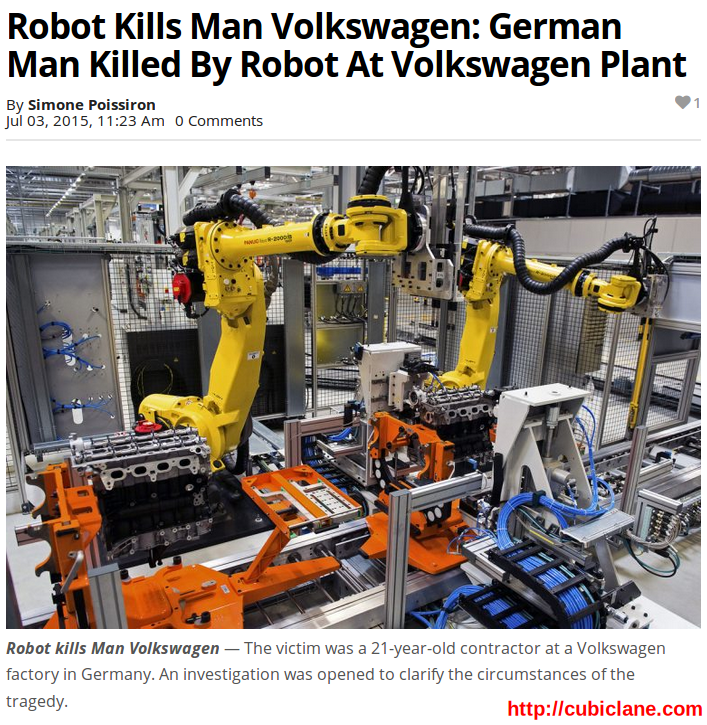
\includegraphics[width=0.74\textwidth]{figures/Telegraph.pdf}
%\end{center}      
%%The robot grabbed the technician and crushed him against a metal plate,                 
%\end{frame}
%%%%%%%%%%%%%%%%%%%%%%%%%%%%%%% 0 %%%%%%%%%%%%%%%%%%%%%%%%%%%%%%%%%%%%%%%%



%%%%%%%%%%%%%%%%%%%%%%%%%%%%%%%% 1.5 %%%%%%%%%%%%%%%%%%%%%%%%%%%%%%%%%%%%%
%\begin{frame}
%\frametitle{{\textcolor{white}{\hspace{0.3cm}Context}}}
%\begin{center}
%\includegraphics[width=0.84\textwidth]{figures/drawing-11.pdf}
%\end{center}    
%\end{frame}
%%%%%%%%%%%%%%%%%%%%%%%%%%%%%%% 1.5 %%%%%%%%%%%%%%%%%%%%%%%%%%%%%%%%%%%%%%














%%%%%%%%%%%%%%%%%%%%%%%%%%%%%%%%%%%%%%%ù
%\begin{frame}
%  \frametitle{{\textcolor{white}{\hspace{0.3cm}Context}}}
%
%
%
%From a well-identified situation \hspace{9mm}...\hspace{17mm}to a complex one
%\begin{columns}
%
%                \column{.47\paperwidth}
%%                \begin{tcolorbox}[colback=white,title=Frictional non-rigid contact]
%                \begin{center}
%                
%                        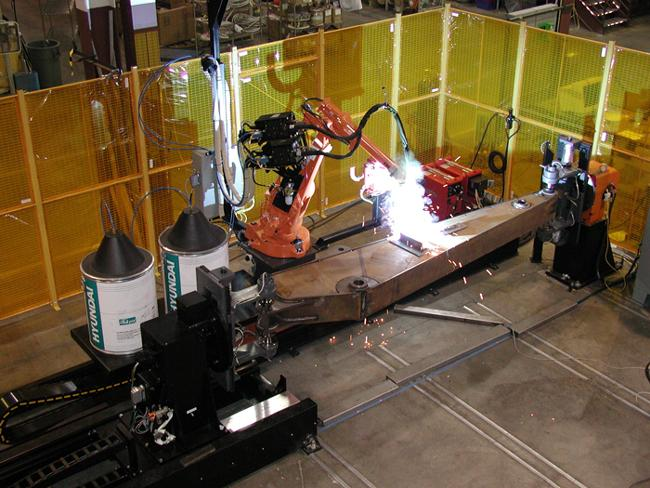
\includegraphics[width=\textwidth ]{figures/well_df_sit.pdf}
%                        
%\setbeamertemplate{itemize items}[triangle]                        
%\begin{itemize}
%\item Static/Known environment 
%\item Known and repetitive trajectories 
%\item Not much considerations for safety 
%\item[\hookrightarrow] No need for much reactivity: Offline planning
%\end{itemize}
%                        
%                        
%                        \end{center}
%%                \end{tcolorbox}
%
%                \column{.47\paperwidth}
%%                \begin{tcolorbox}[colback=white,title=Frictional non-rigid contact]
%                \begin{center}
%                        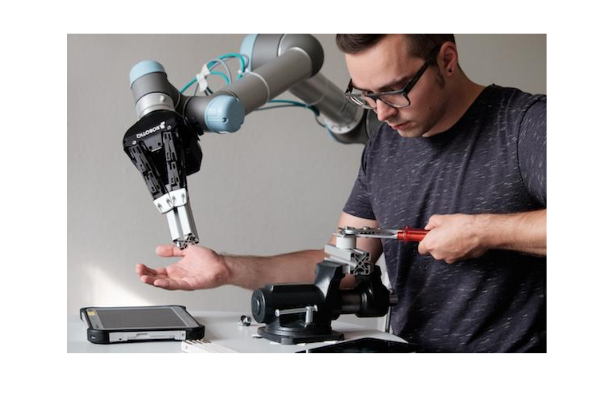
\includegraphics[width=\textwidth ]{figures/complx_sit.pdf}
%\setbeamertemplate{itemize items}[triangle]    
% \vspace{2mm}                    
%\begin{itemize}
%\item Dynamic/Unknown environment
%\item Global mission
%\item Much considerations for safety
%\item[\hookrightarrow] Need for reactivity: \textst{Offline planning}
%\end{itemize}
%
%                        \end{center}
%
%\end{columns}
%
%\end{frame}
%%%%%%%%%%%%%%%%%%%%%%%%%%%%%%%%%%%%%%%%%























%%%%%%%%%%%%%%%%%%%%%%%%%%%%%%%%%%%%%%ù
\begin{frame}
  \frametitle{{\textcolor{white}{\hspace{0.3cm}Context}}}



From a well-identified situation 
\begin{columns}

                \column{.47\paperwidth}
%                \begin{tcolorbox}[colback=white,title=Frictional non-rigid contact]
                \begin{center}
                
                        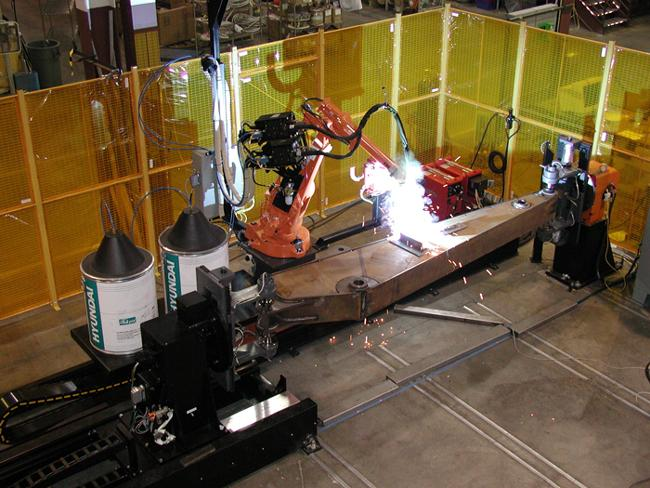
\includegraphics[width=\textwidth ]{figures/well_df_sit.pdf}
                        
\setbeamertemplate{itemize items}[triangle]                        
\begin{itemize}
\item Static/Known environment 
\item Known and repetitive trajectories 
\item Not much considerations for safety 
\item[\hookrightarrow] No need for much reactivity: Offline planning
\end{itemize}
                        
                        
                        \end{center}
%                \end{tcolorbox}

                \column{.47\paperwidth}

\end{columns}

\end{frame}
%%%%%%%%%%%%%%%%%%%%%%%%%%%%%%%%%%%%%%%%




%%%%%%%%%%%%%%%%%%%%%%%%%%%%%%%%%%%%%%ù
\begin{frame}[noframenumbering]
  \frametitle{{\textcolor{white}{\hspace{0.3cm}Context}}}



From a well-identified situation \hspace{9mm}...\hspace{17mm}to a complex one
\begin{columns}

                \column{.47\paperwidth}
%                \begin{tcolorbox}[colback=white,title=Frictional non-rigid contact]
                \begin{center}
                
                        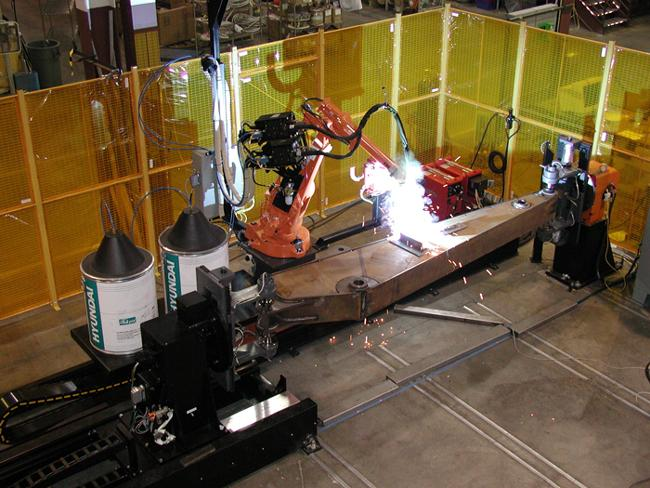
\includegraphics[width=\textwidth ]{figures/well_df_sit.pdf}
                        
\setbeamertemplate{itemize items}[triangle]                        
\begin{itemize}
\item Static/Known environment 
\item Known and repetitive trajectories 
\item Not much considerations for safety 
\item[\hookrightarrow] No need for much reactivity: Offline planning
\end{itemize}
                        
                        
                        \end{center}
%                \end{tcolorbox}

                \column{.47\paperwidth}
%                \begin{tcolorbox}[colback=white,title=Frictional non-rigid contact]
                \begin{center}
                \vspace{-14.6mm}
                        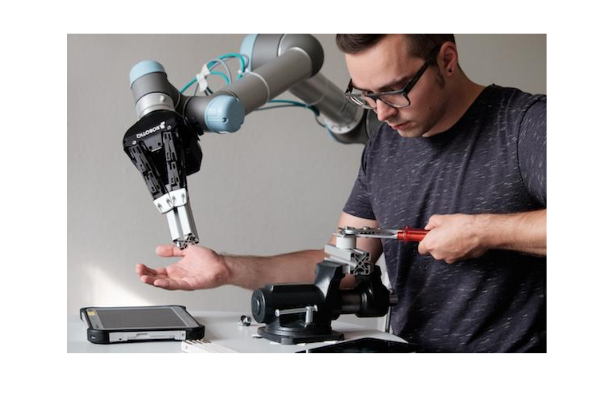
\includegraphics[width=\textwidth ]{figures/complx_sit.pdf}
\setbeamertemplate{itemize items}[triangle]    
 \vspace{2mm}                    
\begin{itemize}
\item Dynamic/Unknown environment
\item Global mission...
\end{itemize}

                        \end{center}

\end{columns}

\end{frame}
%%%%%%%%%%%%%%%%%%%%%%%%%%%%%%%%%%%%%%%%


%%%%%%%%%%%%%%%%%%%%%%%%%%%%%%%%%%%%%%ù
\begin{frame}[noframenumbering]
  \frametitle{{\textcolor{white}{\hspace{0.3cm}Context}}}



From a well-identified situation \hspace{9mm}...\hspace{17mm}to a complex one
\begin{columns}

                \column{.47\paperwidth}
%                \begin{tcolorbox}[colback=white,title=Frictional non-rigid contact]
                \begin{center}
                
                        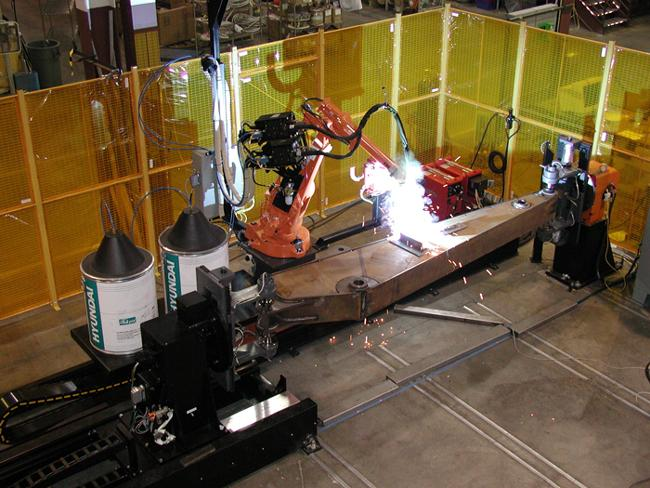
\includegraphics[width=\textwidth ]{figures/well_df_sit.pdf}
                        
\setbeamertemplate{itemize items}[triangle]                        
\begin{itemize}
\item Static/Known environment 
\item Known and repetitive trajectories 
\item Not much considerations for safety 
\item[\hookrightarrow] No need for much reactivity: Offline planning
\end{itemize}
                        
                        
                        \end{center}
%                \end{tcolorbox}

                \column{.47\paperwidth}
%                \begin{tcolorbox}[colback=white,title=Frictional non-rigid contact]
                \begin{center}
                        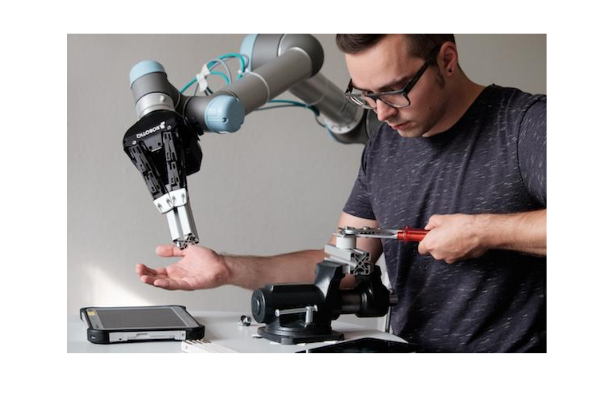
\includegraphics[width=\textwidth ]{figures/complx_sit.pdf}
\setbeamertemplate{itemize items}[triangle]    
 \vspace{2mm}                    
\begin{itemize}
\item Dynamic/Unknown environment
\item Global mission...
\setlength\itemsep{1.5em}
\item[\hookrightarrow] \fbox{\begin{minipage}{15.6em}{\color{red}\textbf{\textit{“collaborative”} robotics, a problem}} \\ {\color{white}aaaaaaa}{\color{red}\textbf{with many dimensions.}}
\end{minipage}}
%\item[\hookrightarrow] Need for reactivity: \textst{Offline planning}
\end{itemize}

                        \end{center}

\end{columns}

\end{frame}
%%%%%%%%%%%%%%%%%%%%%%%%%%%%%%%%%%%%%%%%











%%%%%%%%%%%%%%%%%%%%%%%%%%%%%%%%%%%%%%%ù
%\begin{frame}
%  \frametitle{{\textcolor{white}{\hspace{0.3cm}Collaborative robotics}}}
%
%
%\begin{columns}
%
%\column{.90\paperwidth}
%\begin{table}[]
%\centering
%\resizebox{1\columnwidth}{!}{%
%\begin{tabular}{|l|c|}
%\hline
%\rowcolor[HTML]{00D2CB} 
%\multicolumn{1}{|c|}{\cellcolor[HTML]{00D2CB}{\color[HTML]{000000} \textbf{\begin{tabular}[c]{@{}c@{}}Various aspects \\ to be considered\end{tabular}}}} & {\cellcolor[HTML]{00D2CB}{\color[HTML]{000000} \textbf{Why ?}}}                                                                                                                      \\ \hline
%\rowcolor[HTML]{FFCCC9} 
%\textbf{A. Safety}                                                                                                                                        & \begin{tabular}[c]{@{}c@{}}The robot is strictly forbidden from compromising \\ the physical integrity of the human (ISO/TS 15066).\end{tabular}                          \\ \hline
%\multicolumn{1}{|c|}{\textbf{B. Cognitive aspects}}                                                                                                       & \begin{tabular}[c]{@{}c@{}}Can significantly enhance the quality of the \\ interaction.\end{tabular}                                                       \\ \hline
%\rowcolor[HTML]{FFCCC9} 
%\textbf{C. Reactive control}                                                                                                                              & \begin{tabular}[c]{@{}c@{}}Offline planning is not adapted for \\ dynamic/unknown environments.\end{tabular}                                               \\ \hline
%\textbf{D. Hardware design}                                                                                                                               & \begin{tabular}[c]{@{}c@{}}Must be modified as stiff and heavy structures\\  are not adapted for Human-Robot physical interaction.\end{tabular}            \\ \hline
%\textbf{\begin{tabular}[c]{@{}l@{}}E. Perception \\    \hspace{3mm}  and sensing\end{tabular}}                                                                        & \begin{tabular}[c]{@{}c@{}}A robotic system could for example rely on \\ vision based and torque sensors to reactively adapt its movements.\end{tabular} \\ \hline
%\end{tabular}
%}
%\end{table}
%\end{columns}
%
%
%\begin{itemize}
%\item[\hookrightarrow] \fbox{\begin{minipage}{30.4em}{ \textbf{Addressed dimensions in our work:}
%\setbeamertemplate{itemize items}[triangle]  
%\addtolength{\itemindent}{-3mm}                  
%\begin{itemize}
%\item[\textbf{I.}] {\color{red}\textbf{Problems related to the use of reactive control approaches.}}
%\item[\textbf{II.}] {\color{red}\textbf{The use of safety as a main criteria to control the robot during Human-Robot physical Interaction.}} %
%\end{itemize}}
%\end{minipage}}
%\end{itemize}
%
%
%\end{frame}
%%%%%%%%%%%%%%%%%%%%%%%%%%%%%%%%%%%%%%%%%

%%%%%%%%%%%%%%%%%%%%%%%%%%%%%%%%%%%%%%ù
\begin{frame}[noframenumbering]
  \frametitle{{\textcolor{white}{\hspace{0.3cm}Collaborative robotics -- aspects}}}


\begin{columns}

\column{1.2\paperwidth}

\hspace{-15mm}                       
\includegraphics[width=1.2\paperwidth ]{figures/1.pdf}

\end{columns}




\end{frame}
%%%%%%%%%%%%%%%%%%%%%%%%%%%%%%%%%%%%%%%%

%%%%%%%%%%%%%%%%%%%%%%%%%%%%%%%%%%%%%%ù
\begin{frame}[noframenumbering]
  \frametitle{{\textcolor{white}{\hspace{0.3cm}Collaborative robotics -- aspects}}}


\begin{columns}

\column{1.2\paperwidth}

\hspace{-15mm}               
\includegraphics[width=1.2\paperwidth ]{figures/2.pdf}
      

\end{columns}




\end{frame}
%%%%%%%%%%%%%%%%%%%%%%%%%%%%%%%%%%%%%%%%

%%%%%%%%%%%%%%%%%%%%%%%%%%%%%%%%%%%%%%ù
\begin{frame}[noframenumbering]
  \frametitle{{\textcolor{white}{\hspace{0.3cm}Collaborative robotics -- aspects}}}


\begin{columns}

\column{1.2\paperwidth}

\hspace{-15mm}              
\includegraphics[width=1.2\paperwidth]{figures/3.pdf}
  

\end{columns}




\end{frame}
%%%%%%%%%%%%%%%%%%%%%%%%%%%%%%%%%%%%%%%%


%%%%%%%%%%%%%%%%%%%%%%%%%%%%%%%%%%%%%%ù
\begin{frame}[noframenumbering]
  \frametitle{{\textcolor{white}{\hspace{0.3cm}Collaborative robotics -- aspects}}}


\begin{columns}

\column{1.2\paperwidth}

\hspace{-15mm}               
\includegraphics[width=1.2\paperwidth]{figures/4.pdf}
     

\end{columns}




\end{frame}
%%%%%%%%%%%%%%%%%%%%%%%%%%%%%%%%%%%%%%%%


%%%%%%%%%%%%%%%%%%%%%%%%%%%%%%%%%%%%%%ù
\begin{frame}[noframenumbering]
  \frametitle{{\textcolor{white}{\hspace{0.3cm}Collaborative robotics -- aspects}}}


\begin{columns}

\column{1.2\paperwidth}

\hspace{-15mm}         
\includegraphics[width=1.2\paperwidth ]{figures/5.pdf}
    

\end{columns}




\end{frame}
%%%%%%%%%%%%%%%%%%%%%%%%%%%%%%%%%%%%%%%%













%%%%%%%%%%%%%%%%%%%%%%%%%%%%%%%%%%%%%%ù
\begin{frame}[noframenumbering]
  \frametitle{{\textcolor{white}{\hspace{0.3cm}Collaborative robotics -- aspects}}}


\begin{columns}

\column{.90\paperwidth}

\begin{center}                
\includegraphics[width=0.55\textwidth ]{figures/6.pdf}
\end{center}       

\end{columns}


\begin{itemize}
\item[\hookrightarrow] \fbox{\begin{minipage}{30.4em}{ \textbf{Dimensions addressed in our work:}
\setbeamertemplate{itemize items}[triangle]  
\addtolength{\itemindent}{-3mm}                  
\begin{itemize}
\item[\textbf{I.}] {\color{red}\textbf{Problems related to the use of reactive control loops.}}
\item[\textbf{II.}] {\color{red}\transparent{1.0}\textbf{Safety during Human-Robot physical Interaction.}} %
\end{itemize}}
\end{minipage}}
\end{itemize}
\end{frame}
%%%%%%%%%%%%%%%%%%%%%%%%%%%%%%%%%%%%%%%%





%%%%%%%%%%%%%%%%%%%%%%%%%%%%%%%%%%%%%%ù
\begin{frame}[noframenumbering]
  \frametitle{{\textcolor{white}{\hspace{0.3cm}Reactive control -- aspects}}}


\begin{columns}

\column{.90\paperwidth}

\begin{center}                
\includegraphics[width=0.55\textwidth ]{figures/17.pdf}
\end{center}       

\end{columns}


\begin{itemize}
\item[\hookrightarrow] \fbox{\begin{minipage}{30.4em}{ \textbf{Dimensions addressed in our work:}
\setbeamertemplate{itemize items}[triangle]  
\addtolength{\itemindent}{-3mm}                  
\begin{itemize}
\item[\textbf{I.}] {\color{red}\textbf{Problems related to the use of reactive control loops.}}
\item[\textbf{II.}] {\color{red}\transparent{0.4}\textbf{Safety during Human-Robot physical Interaction.}} %
\end{itemize}}
\end{minipage}}
\end{itemize}
%\hbox{\color{red}\transparent{0.1} MY THESIS}
\end{frame}
%%%%%%%%%%%%%%%%%%%%%%%%%%%%%%%%%%%%%%%%


\begin{frame}
\frametitle{Outline}
  \tableofcontents
\end{frame}

\section{Part I: Reactive control and constraints incompatibility}

%\begin{frame}
%\frametitle{{\textcolor{white}{\hspace{0.3cm}Part I: Reactive control}}}
%\begin{center}     
%{\fontsize{18}{40}\selectfont {\color{violet}\textbf{Part I:}} \textbf{Constraints Incompatibility}}
%\end{center}             
%\end{frame}






\subsection{Reactive control -- the problem}
\begin{frame}
\frametitle{{\textcolor{white}{\hspace{0.3cm}Reactive control -- the problem}}}

\begin{columns}

\column{.98\paperwidth}
\setbeamertemplate{itemize items}[triangle]                        
\begin{itemize}
\item {\color{red}Task and desired trajectory discovered online.}
\item {\color{red}Constraint handled reactively, not by planning} [Katzschmann 2013].
\setlength\itemsep{1em}
\item[$\bullet$] \textbf{Example scenario} [Rubrecht 2012]:

\vspace{1mm}
\begin{center}
\includegraphics[width=0.65\textwidth]{figures/rubrecht_imaj.png}
%\only<1>{\includegraphics[width=0.65\textwidth]{figures/rubrecht_imaj.png}}
%\only<2>{\movie[showcontrols=true,autostart=true,loop=true]{\includegraphics[width=0.75\textwidth]{figures/rubrecht_imaj.png}}{videos/telemach_extrait.mp4}}
\end{center}
\end{itemize}
\end{columns}
\end{frame}









%%A REMETTRE VIABILITE RUBRECHT
%\begin{frame}
%\frametitle{{\textcolor{white}{\hspace{0.3cm}Reactive control}}}
%
%\begin{columns}
%\column{.98\paperwidth}
%\setbeamertemplate{itemize items}[triangle]                        
%\begin{itemize}
%\item \textbf{{\color{red}Question:}} \textbf{How to compute an optimal command that keeps the system into a \textit{viable} state ?}
%
%\item \textit{Viability} [Aubin 2011]: “\textit{A state is viable if starting from this state there exists over an infinite horizon of time a sequence of control inputs that satisfies all its constraints in the future}”.
%
%
%
%\item[$\bullet$] \textbf{Case scenario} [Rubrecht 2012]:
%
%\vspace{1mm}
%\begin{center}
%\movie[showcontrols=true,autostart=true,loop=true]{\includegraphics[width=0.55\textwidth]{figures/rubrecht_imaj.png}}{videos/telemach_extrait.mp4}
%\end{center}
%
%\end{itemize}
%\end{columns}
%\end{frame}












\begin{frame}[noframenumbering]
\frametitle{{\textcolor{white}{\hspace{0.3cm}Reactive control -- the problem}}}

\begin{columns}
\column{.98\paperwidth}

\setbeamertemplate{itemize items}[triangle]                        
\begin{itemize}
\item {\color{red}Reactive control} {\color{blue-violet}\textbf{$\Rightarrow$}} {\color{red}constraint handled reactively, not by planning} [Katzschmann 2013].
\setlength\itemsep{1em}
\item[$\bullet$] {\color{blue-violet}\textbf{\underline{In priority}}}, the system must be able to properly cope with the constraints that correspond to the physical limitations of its actuators:



\begin{columns}
\only<2>{
\column{.59\textwidth}
\vspace{3mm}
\setbeamertemplate{itemize items}[square]
\begin{itemize}
\addtolength{\itemindent}{6mm}
\item Constraint on articular position. 
\item Constraint on articular velocity.
\item Constraint on articular acceleration (torque).
\item Constraint on articular jerk.
\end{itemize}
\column{.5\textwidth}
\vspace{3mm}

\includegraphics[width=0.79\columnwidth]{figures/tele1.pdf}
}

\end{columns}
\end{itemize}


\end{columns}

\end{frame}











\begin{frame}[noframenumbering]
\frametitle{{\textcolor{white}{\hspace{0.3cm}Reactive control -- the problem}}}

\begin{columns}
\column{.98\paperwidth}

\setbeamertemplate{itemize items}[triangle]                        
\begin{itemize}
\item {\color{red}Reactive control} {\color{blue-violet}\textbf{$\Rightarrow$}} {\color{red}constraint handled reactively, not by planning} [Katzschmann 2013].
\setlength\itemsep{1em}
\item[$\bullet$] {\color{blue-violet}\textbf{\underline{In priority}}}, the system must be able to properly cope with the constraints that correspond to the physical limitations of its actuators:



\begin{columns}
\column{.59\textwidth}
\vspace{3mm}
\setbeamertemplate{itemize items}[square]
\begin{itemize}
\addtolength{\itemindent}{6mm}
\item Constraint on articular position. 
\item Constraint on articular velocity.
\item Constraint on articular acceleration (torque).
\item Constraint on articular jerk.
\end{itemize}
\column{.5\textwidth}
\vspace{3mm}

\includegraphics[width=0.79\columnwidth]{figures/tele1.pdf}


\end{columns}
\end{itemize}


\vspace{1mm}

\begin{itemize}
\addtolength{\itemindent}{9mm}
\item[\hookrightarrow] \fbox{\begin{minipage}{31em}{                   
{\color{red}\textbf{Problem I: How to compute at each time-step an optimal control solution that allows the system to cope with its articular constraints while performing at best its assigned task ?}}
}
\end{minipage}}
\end{itemize}
\end{columns}

\end{frame}















%\subsection{Articular constraints implementation}
\begin{frame}
\frametitle{{\textcolor{white}{Articular constraints implementation (the controller)}}}
\hspace{-5mm}

$\bullet$ {\color{blue}\textbf{In an analytical scheme:}} Operational space task projected in the nullspace of the constraints Jacobian [Flacco 2012]. \\
\only<2-4>{
\vspace{2mm}
$\bullet$ {\color{blue}\textbf{In an optimization control scheme}}, e.g.,:
\setbeamertemplate{itemize items}[triangle]  
\begin{itemize}
\addtolength{\itemindent}{2mm}
\item \textbf{Trajectory tracking task} in articular space (on a KUKA LWR4):
\end{itemize}
%$\bullet$ \textbf{Trajectory tracking task} in articular space (on a KUKA LWR4):

\begin{equation}
\textcolor{red}{\boldsymbol{\tau}_{|k}^{{c}^*}}=\argmin \limits_{\textcolor{red}{\boldsymbol{\tau}_{|k}^{c}}, \textcolor{red}{\vect{\ddot{q}}_{|k}^{c}}}  \left\| \vect{\ddot{q}}_{|k}^{~des}-\textcolor{red}{\vect{\ddot{q}}_{|k}^c} \right\|_{Q_t}^2 + \epsilon  \| \textcolor{red}{\boldsymbol{\tau}_{|k}^{c}} \|_{Q_r}^2,
\label{eq:ctrl_pb}
\end{equation}
%With:
%\begin{equation}
%\vect{g}(\textcolor{red}{\vect{\ddot{q}}_{|k}^{c}}) = \vect{\ddot{q}}_{|k}^{~des}-\textcolor{red}{\vect{\ddot{q}}_{|k}^c},
%\label{artaccelerationError}
%\end{equation}
With:
\begin{equation}
\vect{\ddot{q}}_{|k}^{~des} = \textcolor{ao(english)}{K_p} (\vect{q}_{|k}^{*}-\vect{q}_{|k}) - \textcolor{ao(english)}{K_d} \vect{\dot{q}}_{|k}^{*}.
\label{qddot}
\end{equation}}
\only<3-4>{
\textbf{Subject to:} \\
\begin{equation}
M(\vect{q}_{|k}) \textcolor{red}{\vect{\ddot{q}}_{|k}^{c}} + \vect{b}(\vect{q}_{|k},\vect{\dot{q}}_{|k}) = \textcolor{red}{\vect{\tau}_{|k}^{c}},
\label{eq:dyn_eq}
\end{equation}} \\




\only<4>{
\begin{columns}


\column{.5\paperwidth}
\hspace{-30mm}
\begin{subequations}
\label{eq:const_1_literature}
\begin{empheq}[left={}\empheqlbrace]{align}
\vect{q}_{m} & \leq \vect{q}\hspace{2mm}\leq \vect{q}_{M},\label{eq:cnt_lit_1}\\
\vect{\dot{q}}_{m} & \leq \vect{\dot{q}}\hspace{2mm}\leq \vect{\dot{q}}_{M},\label{eq:cnt_lit_2}\\    
{\color{blue-violet}\vect{\ddot{q}}_{m}} & \leq \textcolor{red}{\vect{\ddot{q}}_{|k}^{c}}\leq {\color{blue-violet}\vect{\ddot{q}}_{M}}, \hspace{1mm}({\color{blue-violet}\vect{\tau}_{m}} \leq \textcolor{red}{\vect{\tau}_{|k}^{c}} \leq {\color{blue-violet}\vect{\tau}_{M}})\label{eq:cnt_lit_3}\\
{\color{blue-violet}\vect{\dddot{q}}_{m}}  & \leq \vect{\dddot{q}}\hspace{2mm}\leq {\color{blue-violet}\vect{\dddot{q}}_{M}}.\label{eq:cnt_lit_5}
\end{empheq}
\end{subequations}


\column{.5\paperwidth}
%\hspace{1mm}
%\fbox{\begin{minipage}{12.9em}{
%$\bullet$ {\color{blue-violet}$\vect{\tau}_{M}$} {\color{red}and} {\color{blue-violet}$\vect{\tau}_{m}$} {\color{red}are constant.}\\                   
%$\bullet$ {\color{blue-violet}$\vect{\ddot{q}}_M$}{\color{red}}{\color{red},} {\color{blue-violet}$\vect{\ddot{q}}_m$}{\color{red},} {\color{blue-violet}$\vect{\dddot{q}}_M$}{\color{red}}{\color{red},} {\color{red}and} {\color{blue-violet}$\vect{\dddot{q}}_m$} {\color{red}are} \\ {\color{white}iiii}{\color{red}configuration dependent.}
%%\bullet \hspace{1mm} {\color{red}To simplify,} {\color{blue-violet}$\vect{\ddot{q}}_M$} {\color{red}and} {\color{blue-violet}$\vect{\ddot{q}}_m$} {\color{red}are considered constant.}
%}
%\end{minipage}}
\hspace{1mm}
\fbox{\begin{minipage}{14.9em}{
{\color{red}\textbf{$\longleftarrow$ Depending on how these are formulated, \underline{incompatibility} cases may occur.}}
}
\end{minipage}}

\end{columns}}



\end{frame}















\subsection{Constraints incompatibility, problem illustration (car example)}
\begin{frame}
%\frametitle{{\textcolor{white}{\hspace{0.3cm}Illustration of Problem 1 (car example)}}}
\frametitle{{\textcolor{white}{\hspace{0.3cm}Constraints incompatibility, illustration (car example)}}}
\begin{figure}[!ht]
\centering
\includegraphics[width=0.99\linewidth]{figures/car_exemple_0}
%\caption{Braking phase for the car as it stops before hitting the wall.}
%\label{fig:car_example_1}
\end{figure}
\vspace{2mm}
$\bullet$  \textcolor{red}{\textbf{Constraints}} \textbf{on the car:} 
\begin{subequations}
\label{eq:const_1_literature}
\begin{empheq}[left={}\empheqlbrace]{align}
d & \leq d_{safe},\label{eq:cnt_lit_11}\\
v & \leq v_{Max}, \label{eq:cnt_lit_2}\\    
a & \geq -a_{Max}. \label{eq:cnt_lit_3}
\end{empheq}
\end{subequations}
\end{frame}





\begin{frame}
%\frametitle{{\textcolor{white}{\hspace{0.3cm}Formal and Optimal Solution for Problem 1 (car example)}}}
\frametitle{{\textcolor{white}{\hspace{0.3cm}Constraints incompatibility, optimal solution (car example)}}}
\setbeamertemplate{itemize items}[triangle]  
\begin{itemize}
\addtolength{\itemindent}{-4mm}
\item Case 1: the car starts braking at the optimal time \textcolor{red}{$t$}.
\end{itemize}
\begin{figure}[!ht]
\centering
\includegraphics[width=0.99\linewidth]{figures/car_example_1}
%\caption{Braking phase for the car as it stops before crashing into the wall.}
%\label{fig:car_example_2}
\end{figure}
\vspace{2mm}
$\bullet$  \textcolor{red}{$t$} \textbf{depends on: }
\setbeamertemplate{itemize items}[triangle]
\begin{itemize}
\item The car's position limit \textcolor{red}{$d_{safe}$}. 
\item The car's deceleration limit \textcolor{red}{$-a_{Max}$}. 
\end{itemize}  
\vspace{1mm}
\begin{itemize}
\addtolength{\itemindent}{0mm}
\item[\hookrightarrow] \fbox{\begin{minipage}{27.9em}{                   
{\color{ao(english)}\textbf{Optimal solution w.r.t to the objective and to the constraints.}}
}
\end{minipage}}
\end{itemize}
\end{frame}







%
%%NON OPTIMAL SOLUTION
%\begin{frame}
%\frametitle{{\textcolor{white}{\hspace{0.3cm}Constraints incompatibility, non optimal solution (car example)}}}
%%If t* is not perfectly knows, to cope with the position constraint, the car can react in three different ways: 
%\setbeamertemplate{itemize items}[triangle]  
%\begin{itemize}
%\addtolength{\itemindent}{-4mm}
%\item Case 2: the car starts braking before the optimal time \textcolor{red}{$t$}.
%\end{itemize}
%
%\begin{figure}[!ht]
%\centering
%\includegraphics[width=0.99\linewidth]{figures/car_example_11}
%%\caption{The car starts braking at the optimal time \textcolor{red}{$t$}.}
%%\label{fig:car_example_11}
%\end{figure}
%\vspace{1mm}
%\begin{itemize}
%\addtolength{\itemindent}{0mm}
%\item[\hookrightarrow] \fbox{\begin{minipage}{20.1em}{                   
%{\color{blue}\textbf{Non optimal solution w.r.t to the objective.}}
%}
%\end{minipage}}
%\end{itemize}
%\end{frame}





\begin{frame}
  \begin{columns}
    \column{\dimexpr\paperwidth-4pt}
\frametitle{{\textcolor{white}{\hspace{0.3cm}Constraints incompatibility, no available solution (car example)}}}
%If t* is not perfectly knows, to cope with the position constraint, the car can react in three different ways: 


\setbeamertemplate{itemize items}[triangle]  
\begin{itemize}
\addtolength{\itemindent}{-0mm}
\item Case 3: the car starts braking after the optimal time \textcolor{red}{$t$} $\rightarrow$ \textbf{\textcolor{red}{inevitable Collision !}}
\end{itemize}


\begin{figure}[!ht]
\centering
\includegraphics[width=0.89\linewidth]{figures/car_example_13}
%\caption{Braking phase for the car induced after the optimal time \textcolor{red}{$t$} as it crashes into the wall.}
%\label{fig:car_example_13}
\end{figure}

\vspace{1mm}
\begin{itemize}

\item[\hookrightarrow] \fbox{\begin{minipage}{28.3em}{                   
{\color{red}\textbf{Problem:}} \textbf{\color{red}constraints incompatibility} \textbf{{\color{blue-violet}(position} {\color{black}\textit{VS}} {\color{blue-violet}deceleration)}}}

\end{minipage}}
\end{itemize}


%\item \textbf{Position constraint} \textcolor{red}{incompatibility} with the constraint on \textbf{deceleration capability}.
%\item[\hookrightarrow] \textbf{\textcolor{ao(english)}{Solution:}} the expression of the position constraint should account for the system's deceleration capability.

  \end{columns}
\end{frame}








%SOLUTION CAR EXAMPLE
%\begin{frame}[noframenumbering]
%  \begin{columns}
%    \column{\dimexpr\paperwidth-4pt}
%\frametitle{{\textcolor{white}{\hspace{0.3cm}Constraints incompatibility, no available solution (car example)}}}
%%If t* is not perfectly knows, to cope with the position constraint, the car can react in three different ways: 
%
%\vspace{-1mm}
%\setbeamertemplate{itemize items}[triangle]  
%\begin{itemize}
%\addtolength{\itemindent}{-0mm}
%\item Case 3: the car starts braking after the optimal time \textcolor{red}{$t$} $\rightarrow$ \textbf{\textcolor{red}{inevitable Collision !}}
%\end{itemize}
%
%\vspace{-6mm}
%\hspace{-3mm}
%\begin{figure}
%\includegraphics[width=0.79\linewidth]{figures/car_example_13}
%%\caption{Braking phase for the car induced after the optimal time \textcolor{red}{$t$} as it crashes into the wall.}
%%\label{fig:car_example_13}
%\end{figure}
%
%\vspace{-3mm}
%\begin{itemize}
%\addtolength{\itemindent}{-2mm}
%\item[\hookrightarrow] \fbox{\begin{minipage}{35.3em}{                   
%{\color{ao(english)}\textbf{Solution:}} {\color{red}\textbf{the formulation of the constraint on position should in addition to the state of the system $d$ and $v$, account for the car's deceleration capability $-a_{Max}$.}}
%\vspace{-1mm}
%\begin{subequations}
%\label{eq:const_1_literature}
%\begin{empheq}[left={}\empheqlbrace]{align}
%& \cancel{d \leq d_{safe},} \rightarrow {\color{ao(english)}f(d, v, -a_{Max}) \leq d_{safe}},\label{eq:cnt_lit_11}\\
%& v \leq v_{Max}, \label{eq:cnt_lit_2}\\    
%& a \geq -a_{Max}. \label{eq:cnt_lit_3}
%\end{empheq}
%\end{subequations}
%
%}
%\end{minipage}}
%\end{itemize}
%
%
%%\item \textbf{Position constraint} \textcolor{red}{incompatibility} with the constraint on \textbf{deceleration capability}.
%%\item[\hookrightarrow] \textbf{\textcolor{ao(english)}{Solution:}} the expression of the position constraint should account for the system's deceleration capability.
%
%  \end{columns}
%\end{frame}













\subsection{Articular constraints and the incompatibility problem}
\begin{frame}
\frametitle{{\textcolor{white}{Articular constraints and the incompatibility problem}}}
%the classic approach to do that is based on the extended state of the system at instant $k$ and a local discrete linear approximation of its behaviour within a $\delta t$ time-step duration:  
$\bullet$ \textbf{Naive formulation}, discretization over just {\color{blue}one $\delta t$} time-step:

\begin{subequations}
\label{eq:const_1_literature}
\begin{empheq}[left={}\empheqlbrace]{align}
\vect{q}_{m} & \leq \vect{q}_{|k+\textcolor{blue}{1}} = \vect{q}_{|k} + \textcolor{blue}{\delta t} \vect{\dot{q}}_{|k} + \frac{\textcolor{blue}{\delta t}^{2}}{2} \textcolor{red}{\vect{\ddot{q}}_{|k}^{c}} \leq \vect{q}_{M},\label{eq:cnt_lit_tt1}\\
\vect{\dot{q}}_{m} & \leq \vect{\dot{q}}_{|k+\textcolor{blue}{1}} = \vect{\dot{q}}_{|k} + \textcolor{blue}{\delta t} \textcolor{red}{\vect{\ddot{q}}_{|k}^{c}} \hspace{13mm}\leq \vect{\dot{q}}_{M},\label{eq:cnt_lit_tt2}\\
{\color{blue-violet}\vect{\ddot{q}}_{m}} & \leq \textcolor{red}{\vect{\ddot{q}}_{|k}^{c}}\hspace{35.5mm}\leq {\color{blue-violet}\vect{\ddot{q}}_{M}},\label{eq:cnt_lit_3}\\
{\color{blue-violet}\vect{\dddot{q}}_{m}}  & \leq \vect{\dddot{q}}_{|k+\textcolor{blue}{1}} =  \frac{1}{\textcolor{blue}{\delta t}} (\textcolor{red}{\vect{\ddot{q}}_{|k}^{c}} - \vect{\ddot{q}}_{|k})\hspace{9mm}\leq {\color{blue-violet}\vect{\dddot{q}}_{M}}.\label{eq:cnt_lit_5}
\end{empheq}
\end{subequations}



\begin{itemize}
\addtolength{\itemindent}{-3mm}
\item[\hookrightarrow] \fbox{\begin{minipage}{28.9em}{                   
{\color{blue}\textbf{No consideration for the system's dynamic capabilities for the formulation of (\ref{eq:cnt_lit_tt1}) and (\ref{eq:cnt_lit_tt2}).}}
}
\end{minipage}}


\end{itemize}


\only<2-3>{\vspace{-0mm}
\begin{itemize}
\addtolength{\itemindent}{-3mm}
\item[\hookrightarrow] \fbox{\begin{minipage}{28.9em}{                   
{\color{red}\textbf{{\color{black}Because activated only \textcolor{blue}{one $\delta t$} before reaching their considered limits} {\color{blue-violet}$\rightarrow$} Often results in constraints incompatibilities !}}
}
\end{minipage}}



%\item[\hookrightarrow] \fbox{\begin{minipage}{30em}{                   
%{\color{applegreen}\textbf{Contribution I: new formulations of the articular  constraints that account for the dynamics of the system.}}

%\vspace{2mm}
%\item[\hookrightarrow] \fbox{\begin{minipage}{30em}{                   
%{\color{ao(english)}\textbf{Contribution I: \\
%$\bullet$ New formulations of the articular constraints that account for the \\
%\vspace{2mm}
%{\color{white}i} dynamics of the system are proposed. \\
%$\bullet$ A dynamic optimal control solution for a reactively controlled \\ {\color{white}iii}robotic arm that satisfies all its constraints over an infinite horizon \\ {\color{white}ii} of time is guaranteed at each time-step.}}
%}
%\end{minipage}}

\end{itemize}}




\only<3>{
\begin{itemize}
\addtolength{\itemindent}{-3mm}
\item[\hookrightarrow] \fbox{\begin{minipage}{28.9em}{                   
{\color{ao(english)}\textbf{Formulations of (\ref{eq:cnt_lit_tt1}) and (\ref{eq:cnt_lit_tt2}) should be modified to account for the system's dynamic capabilities.}}
}
\end{minipage}}


\end{itemize}}



\end{frame}





















%\begin{frame}
%\frametitle{{\textcolor{white}{\hspace{0.3cm}Two other possible reactions for the car}}}
%%If t* is not perfectly knows, to cope with the position constraint, the car can react in three different ways: 
%\begin{itemize}
%\item[\textbf{I.}] Case 1: the car starts braking before the optimal time \textcolor{red}{$t$} $\rightarrow$ \textbf{\textcolor{blue}{Non Optimal Solution}}. 
%\begin{figure}[!ht]
%\centering
%\includegraphics[width=0.7\linewidth]{\figurepath/car_example_2}
%\caption{Braking phase for the car in scenario 1 as it stops before hitting the wall.}
%\label{fig:car_example_2}
%\end{figure}
%\item[\textbf{II.}] Case 2: the car starts braking at \textcolor{red}{$t$} $\rightarrow$ \textbf{\textcolor{ao(english)}{Optimal Solution}}. 
%\begin{figure}[!ht]
%\centering
%\includegraphics[width=0.7\linewidth]{\figurepath/car_example_2}
%\caption{Braking phase for the car in scenario 1 as it stops before hitting the wall.}
%\label{fig:car_example_2}
%\end{figure}
%\item[\textbf{III.}] Case 3: the car starts braking after \textcolor{red}{$t$} $\rightarrow$ \textbf{\textcolor{red}{The car inevitably crashes} (Constraints incompatibility problem)}.
%\begin{figure}[!ht]
%\centering
%\includegraphics[width=0.7\linewidth]{\figurepath/car_example_2}
%\caption{Braking phase for the car in scenario 1 as it stops before hitting the wall.}
%\label{fig:car_example_2}
%\end{figure}
%\end{itemize}
%%It is impossible to cope with bothe the car's position and deceleration constraints.   
%\end{frame}
%







%
%\begin{frame}
%\frametitle{{\textcolor{white}{Articular constraints as inequalities}}}
%%the classic approach to do that is based on the extended state of the system at instant $k$ and a local discrete linear approximation of its behaviour within a $\delta t$ time-step duration:  
%$\bullet$ \textbf{Naive formulation}, discretization over just {\color{blue}one $\delta t$} time-step:
%
%\begin{subequations}
%\label{eq:const_1_literature}
%\begin{empheq}[left={}\empheqlbrace]{align}
%\vect{q}_{m} & \leq \vect{q}_{|k+\textcolor{blue}{1}} = \vect{q}_{|k} + \textcolor{blue}{\delta t} \vect{\dot{q}}_{|k} + \frac{\textcolor{blue}{\delta t}^{2}}{2} \textcolor{red}{\vect{\ddot{q}}_{|k}^{c}} \leq \vect{q}_{M},\label{eq:cnt_lit_tt1}\\
%\vect{\dot{q}}_{m} & \leq \vect{\dot{q}}_{|k+\textcolor{blue}{1}} = \vect{\dot{q}}_{|k} + \textcolor{blue}{\delta t} \textcolor{red}{\vect{\ddot{q}}_{|k}^{c}} \hspace{13mm}\leq \vect{\dot{q}}_{M},\label{eq:cnt_lit_tt2}\\    
%{\color{blue-violet}\vect{\ddot{q}}_{m}} & \leq \textcolor{red}{\vect{\ddot{q}}_{|k}^{c}}\hspace{35.5mm}\leq {\color{blue-violet}\vect{\ddot{q}}_{M}},\label{eq:cnt_lit_3}\\
%{\color{blue-violet}\vect{\dddot{q}}_{m}}  & \leq \vect{\dddot{q}}_{|k+\textcolor{blue}{1}} =  \frac{1}{\textcolor{blue}{\delta t}} (\textcolor{red}{\vect{\ddot{q}}_{|k}^{c}} - \vect{\ddot{q}}_{|k})\hspace{9mm}\leq {\color{blue-violet}\vect{\dddot{q}}_{M}}.\label{eq:cnt_lit_5}
%\end{empheq}
%\end{subequations}
%
%
%
%\begin{itemize}
%\addtolength{\itemindent}{-3mm}
%\item[\hookrightarrow] \fbox{\begin{minipage}{28.9em}{                   
%{\color{blue}\textbf{No consideration for the system's dynamic capabilities for the formulation of (\ref{eq:cnt_lit_tt1}) and (\ref{eq:cnt_lit_tt2}).}}
%}
%\end{minipage}}
%
%
%\end{itemize}
%
%
%\vspace{-0mm}
%\begin{itemize}
%\addtolength{\itemindent}{-3mm}
%\item[\hookrightarrow] \fbox{\begin{minipage}{20.9em}{                   
%{\color{red}\textbf{Often results in constraints incompatibilities !}}
%}
%\end{minipage}}
%
%%\item[\hookrightarrow] \fbox{\begin{minipage}{30em}{                   
%%{\color{applegreen}\textbf{Contribution I: new formulations of the articular  constraints that account for the dynamics of the system.}}
%
%%\vspace{2mm}
%\item[\hookrightarrow] \fbox{\begin{minipacnt_lit_tt2ge}{30em}{                   
%{\color{ao(english)}\textbf{Contribution I: \\
%$\bullet$ New formulations of the articular constraints that account for the \\
%\vspace{2mm}
%{\color{white}i} dynamics of the system are proposed. \\
%$\bullet$ A dynamic optimal control solution for a reactively controlled \\ {\color{white}iii}robotic arm that satisfies all its constraints over an infinite horizon \\ {\color{white}ii} of time is guaranteed at each time-step.}}
%}
%\end{minipage}}
%
%\end{itemize}
%
%
%
%
%
%\begin{itemize}
%\addtolength{\itemindent}{-3mm}
%\item[\hookrightarrow] \fbox{\begin{minipage}{28.9em}{                   
%{\color{ao(english)}\textbf{Formulations of (\ref{eq:cnt_lit_tt1}) and (\ref{eq:cnt_lit_tt2}) should be modified to account for the system's dynamic capabilities.}}
%}
%\end{minipage}}
%
%
%\end{itemize}
%
%
%\vspace{5mm}
%$\bullet$ \textbf{2 considered incompatibility Cases}:
%\begin{itemize}
%\item[1.] \fbox{\begin{minipage}{17.5em}
%Constraint on $\vect{q}$ \textcolor{red}{\textbf{$VS$}} Constraints on $\vect{\ddot{q}}$ \& $\vect{\dddot{q}}$.
%\end{minipage}} 
%\item[2.] \fbox{\begin{minipage}{15.1em}
%Constraint on $\vect{\dot{q}}$ \textcolor{red}{\textbf{$VS$}} Constraint on $\vect{\dddot{q}}$.
%\end{minipage}}
%\end{itemize}
%\vspace{0mm}
%\begin{itemize}
%\addtolength{\itemindent}{-3mm}
%\item[\hookrightarrow] \fbox{\begin{minipage}{21.2em}{                   
%{\color{ao(english)}\textbf{Constraints on $\vect{q}$ and $\vect{\dot{q}}$ must be reformulated !}}
%}
%\end{minipage}}
%\end{itemize}
%
%\end{frame}






















%\begin{frame}
%\frametitle{{\textcolor{white}{Articular constraints as inequalities in a control scheme (example)}}}
%$\bullet$ \textbf{Trajectory tracking task} in articular space (on KUKA LWR4):
%\begin{equation}
%\argmin \limits_{\textcolor{red}{\boldsymbol{\tau}_{|k}^{c}}, \textcolor{red}{\vect{\ddot{q}}_{|k}^{c}}}  \left\| \vect{g}\left(\textcolor{red}{\vect{\ddot{q}}_{|k}^{c}}, \vect{\ddot{q}}_{|k}^{~des}\right) \right\|_{Q_t}^2 + \epsilon  \| \textcolor{red}{\boldsymbol{\tau}_{|k}^{c}} \|_{Q_r}^2,
%\label{eq:ctrl_pb}
%\end{equation}
%With:
%\begin{equation}
%\vect{g}(\textcolor{red}{\vect{\ddot{q}}_{|k}^{c}}) = \vect{\ddot{q}}_{|k}^{~des}-\textcolor{red}{\vect{\ddot{q}}_{|k}^c},
%\label{artaccelerationError}
%\end{equation}
%and:
%\begin{equation}
%\vect{\ddot{q}}_{|k}^{~des} = \textcolor{ao(english)}{K_p} (\vect{q}_{|k}^{*}-\vect{q}_{|k}) - \textcolor{ao(english)}{K_d} \vect{\dot{q}}_{|k}^{*}.
%\label{qddot}
%\end{equation}
%\textbf{Subject to:} \\
%\begin{equation}
%M(\vect{q}_{|k}) \textcolor{red}{\vect{\ddot{q}}_{|k}^{c}} + \vect{b}(\vect{q}_{|k},\vect{\dot{q}}_{|k}) = \textcolor{red}{\vect{\tau}_{|k}^{c}},
%\label{eq:dyn_eq}
%\end{equation} \\
%
%
%\begin{columns}
%\column{.5\paperwidth}
%\hspace{-30mm}
%\begin{subequations}
%\label{eq:const_1_literature}
%\begin{empheq}[left={}\empheqlbrace]{align}
%\vect{q}_{m} & \leq \vect{q}\hspace{2mm}\leq \vect{q}_{M},\label{eq:cnt_lit_1}\\
%\vect{\dot{q}}_{m} & \leq \vect{\dot{q}}\hspace{2mm}\leq \vect{\dot{q}}_{M},\label{eq:cnt_lit_2}\\    
%{\color{blue-violet}\vect{\ddot{q}}_{m}} & \leq \textcolor{red}{\vect{\ddot{q}}_{|k}^{c}}\leq {\color{blue-violet}\vect{\ddot{q}}_{M}}, \hspace{1mm}({\color{blue-violet}\vect{\tau}_{m}} \leq \textcolor{red}{\vect{\tau}_{|k}^{c}} \leq {\color{blue-violet}\vect{\tau}_{M}})\label{eq:cnt_lit_3}\\
%{\color{blue-violet}\vect{\dddot{q}}_{m}}  & \leq \vect{\dddot{q}}\hspace{2mm}\leq {\color{blue-violet}\vect{\dddot{q}}_{M}}.\label{eq:cnt_lit_5}
%\end{empheq}
%\end{subequations}
%
%
%\column{.5\paperwidth}
%\hspace{1mm}
%\fbox{\begin{minipage}{12.9em}{
%$\bullet$ {\color{red}If \ref{eq:eq:cnt_lit_1} \& \ref{eq:eq:cnt_lit_2} don't account for} {\color{blue-violet}$\vect{\ddot{q}}_M$}{\color{red}}{\color{red},} {\color{blue-violet}$\vect{\ddot{q}}_m$}{\color{red},} {\color{blue-violet}$\vect{\dddot{q}}_M$}{\color{red}}{\color{red},} {\color{red}and} {\color{blue-violet}$\vect{\dddot{q}}_m$} 
%
%
%%\bullet \hspace{1mm} {\color{red}To simplify,} {\color{blue-violet}$\vect{\ddot{q}}_M$} {\color{red}and} {\color{blue-violet}$\vect{\ddot{q}}_m$} {\color{red}are considered constant.}
%}
%\end{minipage}}














\end{columns}
\end{frame}

























%\subsection{state-of-the-art} %ORIGINAL COMPLETE
%\begin{frame}
%\frametitle{{\textcolor{white}{\hspace{0.3cm}Constraints incompatibilities, state of the art and contribution}}}
%
%\begin{columns}
%\column{\textwidth+5mm}
%$\bullet$ \textbf{State of the art:}
%\setbeamertemplate{itemize items}[triangle]                        
%\begin{itemize}
%\item $[$Lange 2015$]$: Jerk-Limited stopping motion generation.
%\item $[$Park 1998$]$: P-Step-Ahead Predictor (PSAP).
%%\item $[$Tan 2016$]$: The use of MPC to activate constraints a horizon of time ahead.
%\item $[$Rubrecht 2010$]$: Constraints Compliant Control at kinematic-level.
%\end{itemize}
%\end{columns}
%
%
%
%\vspace{1mm}
%\begin{itemize}
%
%\only<2-3>{
%\addtolength{\itemindent}{-3mm}
%\item[\hookrightarrow] \fbox{\begin{minipage}{30.0em}{                   
%{\color{red}\textbf{Existing techniques not adapted to \underline{optimally} solve the constraints incompatibility problem at the \underline{dynamic level} !}}
%}
%\end{minipage}}}
%
%
%%\item[\hookrightarrow] \fbox{\begin{minipage}{30em}{                   
%%{\color{applegreen}\textbf{Contribution I: new formulations of the articular  constraints that account for the dynamics of the system.}}
%
%
%\only<3>{
%\vspace{2mm}
%\item[\hookrightarrow] \fbox{\begin{minipage}{30em}{                   
%{\color{ao(english)}\textbf{Contribution I: \\
%{\color{black}$\bullet$} New formulations of the articular constraints that account for the dynamics of the system are proposed. \\
%%{\color{black}$\bullet$} A dynamic optimal control solution for a reactively controlled \\ {\color{white}iii}robotic arm that satisfies all its constraints over an infinite horizon \\ {\color{white}ii} of time is guaranteed at each time-step.}}
%{\color{black}$\bullet$} A dynamic optimal control solution for a reactively controlled robotic arm that preserves the viability of its state is guaranteed.}}\\
%\textbf{\textit{Viability}} [Aubin 2011]: “\textit{A state is viable if starting from this state there exists over an infinite horizon of time a sequence of control inputs that satisfies all its constraints in the future}”.
%}
%\end{minipage}}}
%
%
%\end{itemize}
%\end{frame}



















%%µµµµµµµµµµµµ
\subsection{Literature}
\begin{frame}
\frametitle{{\textcolor{white}{\hspace{0.3cm}Constraints incompatibilities, state of the art and contribution}}}

\begin{columns}
\column{\textwidth+5mm}

$\bullet$ \textbf{State of the art:}
\setbeamertemplate{itemize items}[triangle]                        
\begin{itemize}
\item $[$Lange 2015$]$: Jerk-Limited stopping motion generation.
\end{itemize}

\end{columns}
\end{frame}









%%µµµµµµµµµµµµ
\begin{frame}[noframenumbering]
\frametitle{{\textcolor{white}{\hspace{0.3cm}Constraints incompatibilities, state of the art and contribution}}}

\begin{columns}
\column{\textwidth+5mm}

$\bullet$ \textbf{State of the art:}
\setbeamertemplate{itemize items}[triangle]                        
\begin{itemize}
\item $[$Lange 2015$]$: Jerk-Limited stopping motion generation.
\end{itemize}

\vspace{1mm}
\begin{itemize}

\addtolength{\itemindent}{-3mm}
\item[\hookrightarrow] \fbox{\begin{minipage}{30.0em}{                   
\textbf{\textit{Viability}} [Aubin 2011]: “\textit{A state is viable if starting from this state there exists {\color{red}over an infinite horizon of time} a sequence of control inputs {\color{red}that satisfies all its constraints in the future}}”.
}
\end{minipage}}



\end{itemize}
\end{columns}
\end{frame}







%%µµµµµµµµµµµµ
\begin{frame}[noframenumbering]
\frametitle{{\textcolor{white}{\hspace{0.3cm}Constraints incompatibilities, state of the art and contribution}}}

\begin{columns}
\column{\textwidth+5mm}

$\bullet$ \textbf{State of the art:}
\setbeamertemplate{itemize items}[triangle]                        
\begin{itemize}
\item $[$Lange 2015$]$: Jerk-Limited stopping motion generation.
\end{itemize}

\vspace{1mm}
\begin{itemize}

\addtolength{\itemindent}{-3mm}
\item[\hookrightarrow] \fbox{\begin{minipage}{30.0em}{                   
\textbf{\textit{Viability}} [Aubin 2011]: “\textit{A state is viable if starting from this state there exists {\color{red}over an infinite horizon of time} a sequence of control inputs {\color{red}that satisfies all its constraints in the future}}”.
}
\end{minipage}}
\end{itemize}

\setbeamertemplate{itemize items}[triangle]                        
\begin{itemize}
\item $[$Park 1998$]$: P-Step-Ahead Predictor (PSAP).
\item $[$Rubrecht 2010$]$: Constraints Compliant Control at kinematic-level.
\end{itemize}

\end{columns}
\end{frame}










%%µµµµµµµµµµµµ
\begin{frame}[noframenumbering]
\frametitle{{\textcolor{white}{\hspace{0.3cm}Constraints incompatibilities, state of the art and contribution}}}

\begin{columns}
\column{\textwidth+5mm}

$\bullet$ \textbf{State of the art:}
\setbeamertemplate{itemize items}[triangle]                        
\begin{itemize}
\item $[$Lange 2015$]$: Jerk-Limited stopping motion generation.
\end{itemize}

\vspace{1mm}
\begin{itemize}

\addtolength{\itemindent}{-3mm}
\item[\hookrightarrow] \fbox{\begin{minipage}{30.0em}{                   
\textbf{\textit{Viability}} [Aubin 2011]: “\textit{A state is viable if starting from this state there exists {\color{red}over an infinite horizon of time} a sequence of control inputs {\color{red}that satisfies all its constraints in the future}}”.
}
\end{minipage}}
\end{itemize}

\setbeamertemplate{itemize items}[triangle]                        
\begin{itemize}
\item $[$Park 1998$]$: P-Step-Ahead Predictor (PSAP).
\item $[$Rubrecht 2010$]$: Constraints Compliant Control at kinematic-level.
\end{itemize}


\vspace{1mm}
\begin{itemize}
\addtolength{\itemindent}{-3mm}
\item[\hookrightarrow] \fbox{\begin{minipage}{30.0em}{                   
{\color{red}\textbf{Existing techniques not adapted to \underline{optimally} solve the constraints incompatibility problem at the \underline{dynamic level} !}}
}
\end{minipage}}
\end{itemize}

\end{columns}
\end{frame}













%%µµµµµµµµµµµµ
\begin{frame}[noframenumbering]
\frametitle{{\textcolor{white}{\hspace{0.3cm}Constraints incompatibilities, state of the art and contribution}}}

\begin{columns}
\column{\textwidth+5mm}

$\bullet$ \textbf{State of the art:}
\setbeamertemplate{itemize items}[triangle]                        
\begin{itemize}
\item $[$Lange 2015$]$: Jerk-Limited stopping motion generation.
\end{itemize}

\vspace{1mm}
\begin{itemize}

\addtolength{\itemindent}{-3mm}
\item[\hookrightarrow] \fbox{\begin{minipage}{30.0em}{                   
\textbf{\textit{Viability}} [Aubin 2011]: “\textit{A state is viable if starting from this state there exists {\color{red}over an infinite horizon of time} a sequence of control inputs {\color{red}that satisfies all its constraints in the future}}”.
}
\end{minipage}}
\end{itemize}

\setbeamertemplate{itemize items}[triangle]                        
\begin{itemize}
\item $[$Park 1998$]$: P-Step-Ahead Predictor (PSAP).
\item $[$Rubrecht 2010$]$: Constraints Compliant Control at kinematic-level.
\end{itemize}


\vspace{1mm}
\begin{itemize}
\addtolength{\itemindent}{-3mm}
\item[\hookrightarrow] \fbox{\begin{minipage}{30.0em}{                   
{\color{red}\textbf{Existing techniques not adapted to \underline{optimally} solve the constraints incompatibility problem at the \underline{dynamic level} !}}
}
\end{minipage}}
\end{itemize}

\begin{itemize}
\addtolength{\itemindent}{-3mm}
\item[\hookrightarrow] \fbox{\begin{minipage}{30.0em}{                   
{\color{ao(english)}\textbf{Contribution I: \\
{\color{black}$\bullet$} New formulations of the articular position \& velocity constraints that account for the dynamic capabilities of the system are proposed. \\
{\color{black}$\bullet$} A dynamic optimal control solution for a reactively controlled robotic arm that preserves the viability of its state is guaranteed.}}
}
\end{minipage}}
\end{itemize}


\end{columns}
\end{frame}





%%%%%%IIIIIIII
%\subsection{Constraints incompatibility on a reactively controlled robotic arm.}
%\begin{frame}
%\frametitle{{\textcolor{white}{\hspace{0.2cm}Same problem on reactively controlled robots}}}
%
%  \begin{columns}
%    \column{\dimexpr\paperwidth-4pt}
%\setbeamertemplate{itemize items}[triangle] 
%\begin{itemize}
%\begin{columns}
%\column{.5\paperwidth}
%\begin{center}
%
%\vspace{0.5mm}
%\hspace{5mm}
%\only<1>{\movie[showcontrols=true,autostart=true]{\includegraphics[width=0.9\textwidth]{videos/constr_comp.png}}{videos/constr_com-5.mp4}}
%\\
%%\begin{flushleft}
%%Dissipation of the unconstrained kinetic energy of the robot end-effector in the direction of the considered obstacle during a collision phase.
%%\end{flushleft}
%\vspace{-1.5mm}
%\hspace{3mm}
%
%\begin{equation}
%M(\textcolor{blue}{\vect{q}_{|k}}) \textcolor{red}{\vect{\ddot{q}}_{|k}^{c}} + \vect{b}(\textcolor{blue}{\vect{q}_{|k}}, \vect{\dot{q}}_{|k}) = \textcolor{red}{\vect{\tau}_{|k}^{c}},
%\end{equation}
%
%\vspace{-1mm}
%\begin{itemize}
%\addtolength{\itemindent}{5mm}
%\item[\hookrightarrow] \fbox{\begin{minipage}{18.9em}{
%\bullet \hspace{1mm} {\color{red}\textbf{$\vect{\tau}_{M}$ and $\vect{\tau}_{m}$ are constant.}}\\                   
%\bullet  \hspace{1mm} {\color{red}\textbf{$\vect{\ddot{q}}_M$ and $\vect{\ddot{q}}_m$ are configuration dependent.}}
%}
%\end{minipage}}
%
%\end{itemize}
%
%\end{center}
%
%\column{.5\textwidth}
%
%\hspace{13mm}
%\vspace{0.5mm}
%\includegraphics[width=0.51\columnwidth]{figures/ang}
%
%%\begin{flushleft}
%%Dissipation of the constrained kinetic energy of the end-effector in the direction of the considered obstacle during a collision phase.
%%\end{flushleft}
%\hspace{14mm}
%\vspace{-2.5mm}
%\setbeamertemplate{itemize items}[triangle]
%\begin{itemize}
%\item Instantaneous deceleration capability:
%\end{itemize}
%\vspace{1mm}
%\hspace{2mm}
%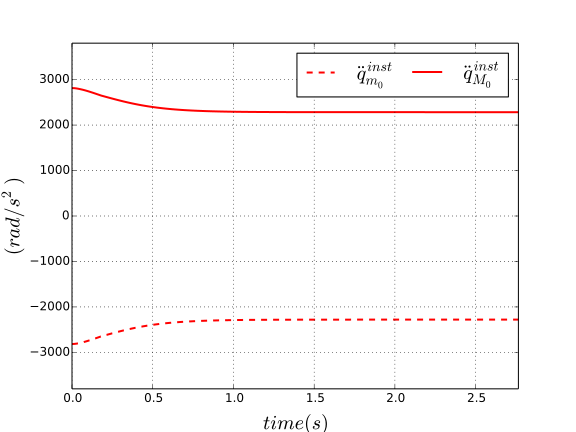
\includegraphics[width=0.79\columnwidth]{figures/instant_articular_acceleration_capability.pdf}
%
%
%
%\end{columns}
%\end{itemize}
%  \end{columns}
%
%
%\end{frame}
%%%%%%IIIIII






\subsection{Constraints on articular position/velocity, naive VS new formulations}
\begin{frame}
\frametitle{{\textcolor{white}{\hspace{0.2cm}Test case scenario for comparing constraints formulations}}}
 
\begin{columns}
\column{\dimexpr\paperwidth-4pt}
    
\setbeamertemplate{itemize items}[triangle]    
\begin{itemize}
\addtolength{\itemindent}{1mm}
\item \textbf{The new formulations to be introduced are compared to the naive ones.}
\item The dynamic optimization control scheme is used.
\item Trajectory traking task in articular space.
\item Control time-step $= 1~ms$.
\item Only the movement of joint $0$ is constrained.
\end{itemize}    
\vspace{5mm}
\begin{columns}
\column{.55\paperwidth}



\begin{center}

\vspace{-15mm}
\hspace{5mm}
\only<1>{\movie[showcontrols=true,autostart=true,loop=true]{\includegraphics[width=0.7\textwidth]{videos/constr_comp.png}}{videos/constr_com-5.mp4}}


%\\
%%\begin{flushleft}
%%Dissipation of the unconstrained kinetic energy of the robot end-effector in the direction of the considered obstacle during a collision phase.
%%\end{flushleft}
%\vspace{-1.5mm}
%\hspace{3mm}
%
%\begin{equation}
%M(\textcolor{blue}{\vect{q}_{|k}}) \textcolor{red}{\vect{\ddot{q}}_{|k}^{c}} + \vect{b}(\textcolor{blue}{\vect{q}_{|k}}, \vect{\dot{q}}_{|k}) = \textcolor{red}{\vect{\tau}_{|k}^{c}},
%\end{equation}
%
%\vspace{-1mm}
%\begin{itemize}
%\addtolength{\itemindent}{5mm}
%\item[\hookrightarrow] \fbox{\begin{minipage}{18.9em}{
%\bullet \hspace{1mm} {\color{red}\textbf{$\vect{\tau}_{M}$ and $\vect{\tau}_{m}$ are constant.}}\\                   
%\bullet  \hspace{1mm} {\color{red}\textbf{$\vect{\ddot{q}}_M$ and $\vect{\ddot{q}}_m$ are configuration dependent.}}
%}
%\end{minipage}}
%
%\end{itemize}

\end{center}

\column{.45\paperwidth}
\hspace{-5mm}
\vspace{5mm}
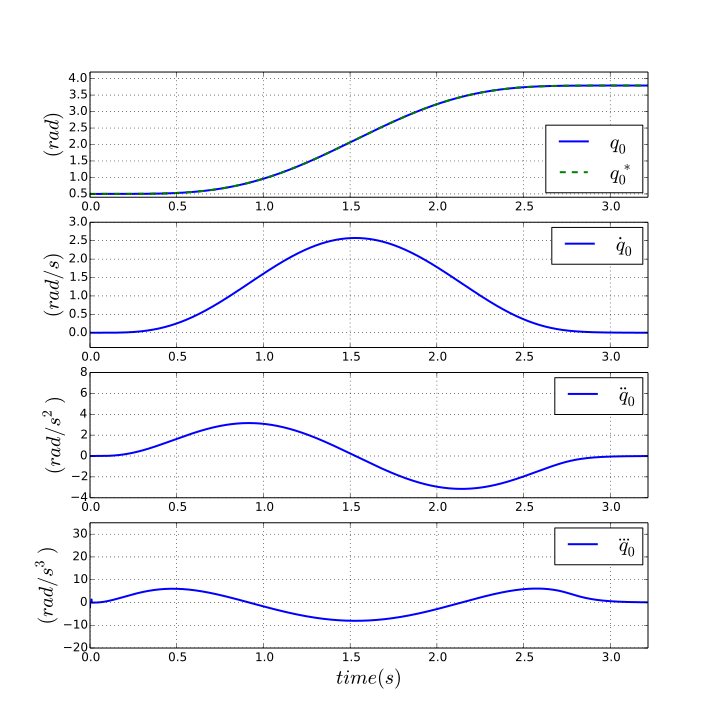
\includegraphics[width=0.98\columnwidth]{figures/No_constr_move.pdf}

%
%\hspace{13mm}
%\vspace{0.5mm}
%\includegraphics[width=0.51\columnwidth]{figures/ang}
%
%%\begin{flushleft}
%%Dissipation of the constrained kinetic energy of the end-effector in the direction of the considered obstacle during a collision phase.
%%\end{flushleft}
%\hspace{14mm}
%\vspace{-2.5mm}
%\setbeamertemplate{itemize items}[triangle]
%\begin{itemize}
%\item Instantaneous deceleration capability:
%\end{itemize}
%\vspace{1mm}
%\hspace{2mm}
%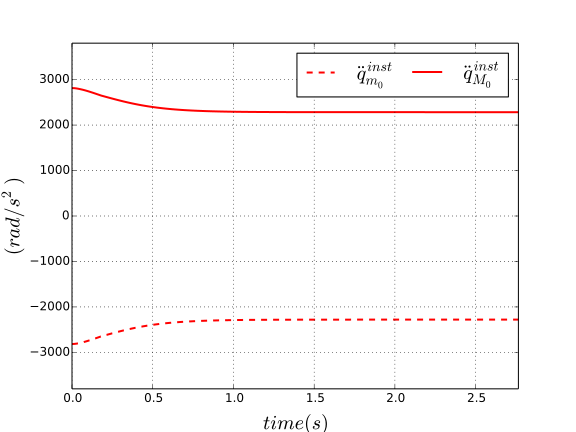
\includegraphics[width=0.79\columnwidth]{figures/instant_articular_acceleration_capability.pdf}



\end{columns}

  \end{columns}


\end{frame}












%%PEUT ETRE A REMETTRE
%\begin{frame}
%\frametitle{{\textcolor{white}{The controller}}}
%$\bullet$ \textbf{Trajectory tracking task} in articular space (on KUKA LWR4):
%\begin{equation}
%\argmin \limits_{\textcolor{red}{\boldsymbol{\tau}_{|k}^{c}}, \textcolor{red}{\vect{\ddot{q}}_{|k}^{c}}}  \left\| \vect{\ddot{q}}_{|k}^{~des}-\textcolor{red}{\vect{\ddot{q}}_{|k}^c} \right\|_{Q_t}^2 + \epsilon  \| \textcolor{red}{\boldsymbol{\tau}_{|k}^{c}} \|_{Q_r}^2,
%\label{eq:ctrl_pb}
%\end{equation}
%%With:
%%\begin{equation}
%%\vect{g}(\textcolor{red}{\vect{\ddot{q}}_{|k}^{c}}) = \vect{\ddot{q}}_{|k}^{~des}-\textcolor{red}{\vect{\ddot{q}}_{|k}^c},
%%\label{artaccelerationError}
%%\end{equation}
%With:
%\begin{equation}
%\vect{\ddot{q}}_{|k}^{~des} = \textcolor{ao(english)}{K_p} (\vect{q}_{|k}^{*}-\vect{q}_{|k}) - \textcolor{ao(english)}{K_d} \vect{\dot{q}}_{|k}^{*}.
%\label{qddot}
%\end{equation}
%\textbf{Subject to:} \\
%\begin{equation}
%M(\vect{q}_{|k}) \textcolor{red}{\vect{\ddot{q}}_{|k}^{c}} + \vect{b}(\vect{q}_{|k},\vect{\dot{q}}_{|k}) = \textcolor{red}{\vect{\tau}_{|k}^{c}},
%\label{eq:dyn_eq}
%\end{equation} \\
%\begin{subequations}
%\label{eq:const_1_literature}
%\begin{empheq}[left={}\empheqlbrace]{align}
%\vect{q}_{m} & \leq \vect{q}\hspace{2mm}\leq \vect{q}_{M},\label{eq:cnt_lit_1}\\
%\vect{\dot{q}}_{m} & \leq \vect{\dot{q}}\hspace{2mm}\leq \vect{\dot{q}}_{M},\label{eq:cnt_lit_2}\\    
%{\color{blue-violet}\vect{\ddot{q}}_{m}} & \leq \textcolor{red}{\vect{\ddot{q}}_{|k}^{c}}\leq {\color{blue-violet}\vect{\ddot{q}}_{M}},\label{eq:cnt_lit_3}\\
%{\color{blue-violet}\vect{\dddot{q}}_{m}}  & \leq \vect{\dddot{q}}\hspace{2mm}\leq {\color{blue-violet}\vect{\dddot{q}}_{M}}.\label{eq:cnt_lit_5}
%\end{empheq}
%\end{subequations}
%\end{frame}





\begin{frame}
\frametitle{{\textcolor{white}{Constraint on articular position: naive \textit{VS} new formulation}}}
%the classic approach to do that is based on the extended state of the system at instant $k$ and a local discrete linear approximation of its behaviour within a $\delta t$ time-step duration:  
\hspace{-5mm}
$\bullet$ {\color{black}\textbf{Naive formulation}} [Park 1998]:
\begin{equation}
\vect{q}_{|k+\textcolor{blue}{1}} = \vect{q}_{|k} + \textcolor{blue}{\delta t} \vect{\dot{q}}_{|k} + \frac{\textcolor{blue}{\delta t}^{2}}{2} \textcolor{red}{\vect{\ddot{q}}_{|k}^{c}} \leq \vect{q}_{M},
\end{equation}

\setbeamertemplate{itemize items}[triangle]
\begin{itemize}
\addtolength{\itemindent}{3mm}
\item Discretization over only {\color{blue}one $\delta t$} time-step.
\setlength\itemsep{-0.1em} 
\item Accounts for the system's state $\vect{q}_{|k}$, $\vect{\dot{q}}_{|k}$ \textbf{{\color{red}and not}} for its dynamic capabilities {\color{blue-violet}$\vect{\ddot{q}}_{m}$}, {\color{blue-violet}$\vect{\dddot{q}}_{m}$} and {\color{blue-violet}$\vect{\dddot{q}}_{M}$}.
\end{itemize}

\vspace{0mm}
\begin{itemize}
\addtolength{\itemindent}{-1mm}
\item[\hookrightarrow] \fbox{\begin{minipage}{18em}{                   
{\color{red}\textbf{Often results in incompatibility issues !}}
}
\end{minipage}}
\end{itemize}
\vspace{5mm}
\hspace{-5mm}





\only<2>{
$\bullet$ {\color{blue}\textbf{New proposed formulation}}:
\begin{equation}
f(\vect{q}_{|k}, \vect{\dot{q}}_{|k}, {\color{blue-violet}\vect{\ddot{q}}_{m}}, {\color{blue-violet}\vect{\dddot{q}}_{m}}, {\color{blue-violet}\vect{\dddot{q}}_{M}}, {\color{blue}n_i \delta t})\leq \vect{q}_{M},
\end{equation}

\setbeamertemplate{itemize items}[triangle]
\begin{itemize}
\addtolength{\itemindent}{3mm}
\item Discretization over {\color{blue} $n_i \delta t$} time-steps. 
\setlength\itemsep{-0.1em} 
\item Accounts for both the system's state $\vect{q}_{|k}$, $\vect{\dot{q}}_{|k}$ \textbf{{\color{ao(english)}and also}} for its dynamic capabilities {\color{blue-violet}$\vect{\ddot{q}}_{m}$}, {\color{blue-violet}$\vect{\dddot{q}}_{m}$} and {\color{blue-violet}$\vect{\dddot{q}}_{M}$}.
\end{itemize}
\vspace{0mm}
\begin{itemize}
\addtolength{\itemindent}{-1mm}
\item[\hookrightarrow] \fbox{\begin{minipage}{28em}{                   
{\color{ao(english)}\textbf{No incompatibility issues with the constraints on $\vect{\ddot{q}}$ and $\vect{\dddot{q}}$.}}
}
\end{minipage}}
\end{itemize}
}


\end{frame}













\begin{frame}
\frametitle{{\textcolor{white}{Constraint on articular position: naive \textit{VS} new formulation} -- Results}}
\hspace{-8mm}
$\bullet$ {\color{black}\textbf{Using the naive formulation of the articular position constraint:}}
\setbeamertemplate{itemize items}[triangle]
\begin{itemize}

\item {\color{red}No available control solution to cope with the joint position constraint within one $\delta t$ time-step considering the constraints on the articular deceleration and jerk.}
\end{itemize}
\only<2>{
\vspace{2mm}
\hspace{-8mm}
$\bullet$ {\color{blue}\textbf{\underline{Using the new formulation of the articular position constraint:}}}
\vspace{1mm}
\begin{columns}
\column{.3\paperwidth}
\hspace{-1mm}
$\bullet$ {\color{blue-violet}\textbf{All constraints on:}}
\begin{itemize}
\item Articular position
\item Articular deceleration
\item Articular jerk
\end{itemize}
\begin{itemize}
\addtolength{\itemindent}{-4mm}
\item[\hookrightarrow] \fbox{\begin{minipage}{9.9em}{                   
{\color{ao(english)}\textbf{Are all simultaneously satisfied.}}

}
\end{minipage}}
\end{itemize}
\column{.6\paperwidth}
{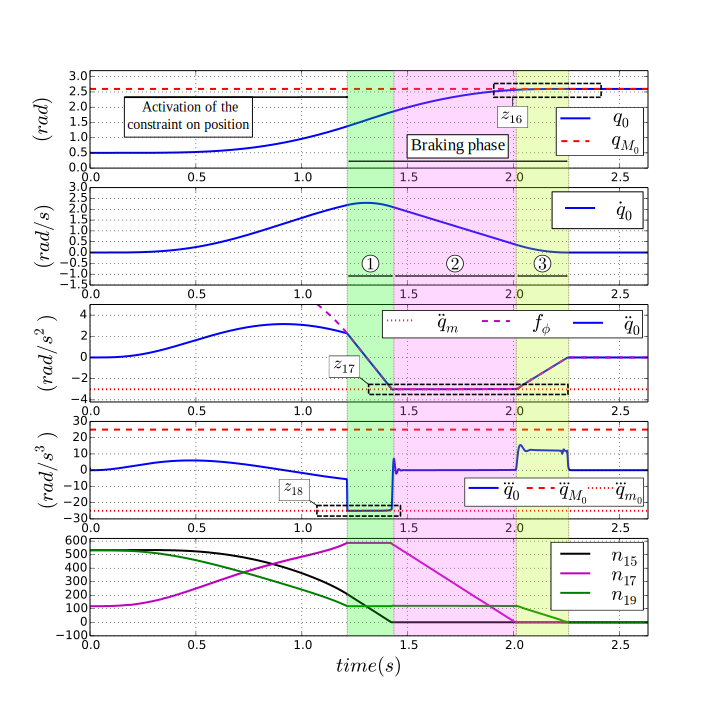
\includegraphics[width=0.95\columnwidth]{figures/11_Posi_constr_jerk_acc_comp_complete_formula_3}} 


\end{columns}
}
\end{frame}






































%
%\begin{frame}
%\frametitle{{\textcolor{white}{Incompatibility cases related to the constraints on the robot's joint physical limitations}}}
%%the classic approach to do that is based on the extended state of the system at instant $k$ and a local discrete linear approximation of its behaviour within a $\delta t$ time-step duration:  
%$\bullet$ \textbf{Naive formulation} [Park 1998]:
%\begin{subequations}
%\label{eq:const_1_literature}
%\begin{empheq}[left={}\empheqlbrace]{align}
%\vect{q}_{m} & \leq \vect{q}_{|k+\textcolor{blue}{1}} = \vect{q}_{|k} + \textcolor{blue}{\delta t} \vect{\dot{q}}_{|k} + \frac{\textcolor{blue}{\delta t}^{2}}{2} \textcolor{red}{\vect{\ddot{q}}_{|k}^{c}} \leq \vect{q}_{M},\label{eq:cnt_lit_1}\\
%\vect{\dot{q}}_{m} & \leq \vect{\dot{q}}_{|k+\textcolor{blue}{1}} = \vect{\dot{q}}_{|k} + \textcolor{blue}{\delta t} \textcolor{red}{\vect{\ddot{q}}_{|k}^{c}} \hspace{13mm}\leq \vect{\dot{q}}_{M},\label{eq:cnt_lit_2}\\    
%\vect{\ddot{q}}_{m} & \leq \textcolor{red}{\vect{\ddot{q}}_{|k}^{c}}\hspace{35.5mm}\leq \vect{\ddot{q}}_{M},\label{eq:cnt_lit_3}\\
%\vect{\dddot{q}}_{m}  & \leq \vect{\dddot{q}}_{|k+\textcolor{blue}{1}} =  \frac{1}{\textcolor{blue}{\delta t}} (\textcolor{red}{\vect{\ddot{q}}_{|k}^{c}} - \vect{\ddot{q}}_{|k})\hspace{9mm}\leq \vect{\dddot{q}}_{M}.\label{eq:cnt_lit_5}
%\end{empheq}
%\end{subequations}
%\hspace{3mm}\rightarrow \textcolor{red}{\textbf{Often results in Incompatibility issues !}} \\
%\vspace{2mm}
%$\bullet$ \textbf{4 Incompatibility Cases:}
%\begin{itemize}
%\item[1.] Constraint on $\vect{q}$ \textcolor{red}{\textbf{$VS$}} Constraint on $\vect{\ddot{q}}$.
%\item[2.] Constraint on $\vect{q}$ \textcolor{red}{\textbf{$VS$}} Constraint on $\vect{\dddot{q}}$.
%\item[3.] \fbox{\begin{minipage}{17.5em}
%Constraint on $\vect{q}$ \textcolor{red}{\textbf{$VS$}} Constraints on $\vect{\ddot{q}}$ \& $\vect{\dddot{q}}$.
%\end{minipage}} 
%\item[4.] \fbox{\begin{minipage}{15.1em}
%Constraint on $\vect{\dot{q}}$ \textcolor{red}{\textbf{$VS$}} Constraint on $\vect{\dddot{q}}$.
%\end{minipage}}
%\end{itemize}
%{\small\hspace{3mm}\rightarrow \textcolor{blue}{\textbf{Solution: Constraints on $\vect{q}$ and $\vect{\dot{q}}$ must be reformulated !}} [Rubrecht 2010]}.
%\end{frame}
%
%
%
%
%
%
%
%
%
%
%
%\begin{frame}
%\frametitle{{\textcolor{white}{Incompatibility case related to the constraint on articular position $\vect{q}$}}}
%$\bullet$ \textcolor{red}{\textbf{Naive}} formulation of the constraint on $\vect{q}$
%\begin{subequations}
%\label{eq:const_1_literature}
%\begin{empheq}[left={}\empheqlbrace]{align}
%\frac{2}{\textcolor{blue}{\delta t}^2} (\textcolor{blue-violet}{\vect{q}_{m}}-\vect{q}_{|k}-\textcolor{blue}{\delta t} \vect{\dot{q}}_{|k}) &\leq \textcolor{red}{\vect{\ddot{q}}_{|k}^{c}} \leq \frac{2}{\textcolor{blue}{\delta t}^2} (\textcolor{blue-violet}{\vect{q}_{M}}-\vect{q}_{|k}-\textcolor{blue}{\delta t} \vect{\dot{q}}_{|k}), \label{eq:cnt_lit_111}\\
%\textcolor{blue-violet}{\vect{\ddot{q}}_{m}} & \leq \textcolor{red}{\vect{\ddot{q}}_{|k}^{c}} \leq \textcolor{blue-violet}{\vect{\ddot{q}}_{M}}.\label{eq:cnt_lit_333}
%\end{empheq}
%\end{subequations}
%\hspace{3mm}\rightarrow \textcolor{red}{\textbf{No optimal solution available for the control problem.}} \\
%\vspace{6mm}
%$\bullet$ \textcolor{red}{\textbf{New}} formulation of the constraint on $\vect{q}$: \\
%
%\vspace{2mm}
%\begin{subequations}
%\resizebox{0.95\hsize}{!}{%
%\label{eq:const_1_literature}
%\begin{empheq}[left={}\empheqlbrace \hspace{5mm} ]{align}
%f_{\chi}(\textcolor{blue-violet}{q_m}, \textcolor{blue-violet}{\dddot{q}_M}, \textcolor{blue-violet}{\ddot{q}_M}, \textcolor{blue-violet}{\dddot{q}_m}, \textcolor{blue}{n_{16}}, \textcolor{blue}{n_{18}}, \textcolor{blue}{n_{20}}) &\leq \textcolor{red}{\ddot{q}_{|k}^{c}} \leq f_{\phi}(\textcolor{blue-violet}{q_M}, \textcolor{blue-violet}{\dddot{q}_m}, \textcolor{blue-violet}{\ddot{q}_m}, \textcolor{blue-violet}{\dddot{q}_M}, \textcolor{blue}{n_{15}}, \textcolor{blue}{n_{17}}, \textcolor{blue}{n_{19}}),  \textcolor{white}{testttt}\label{eq:cnt_lit_1}\\  
%\textcolor{blue-violet}{\vect{\ddot{q}}_{m}}  &\leq \textcolor{red}{\vect{\ddot{q}}_{|k}^{c}}\leq \textcolor{blue-violet}{\vect{\ddot{q}}_{M}},\label{eq:cnt_lit_3}\\
%\textcolor{blue-violet}{\vect{\dddot{q}}_{m}} \textcolor{blue}{\delta t}+\vect{\ddot{q}}_{|k} &\leq \textcolor{red}{\vect{\ddot{q}}_{|k}^{c}} \leq \textcolor{blue-violet}{\vect{\dddot{q}}_{M}} \textcolor{blue}{\delta t}+\vect{\ddot{q}}_{|k}. \label{eq:cnt_lit_5}
%\end{empheq}
%}
%\end{subequations} \\
%\vspace{2mm}
%\hspace{3mm}{\small \rightarrow \textcolor{ao(english)}{\textbf{An optimal solution for the control problem is guaranteed at each time-step.}} }
%%\begin{center}
%%{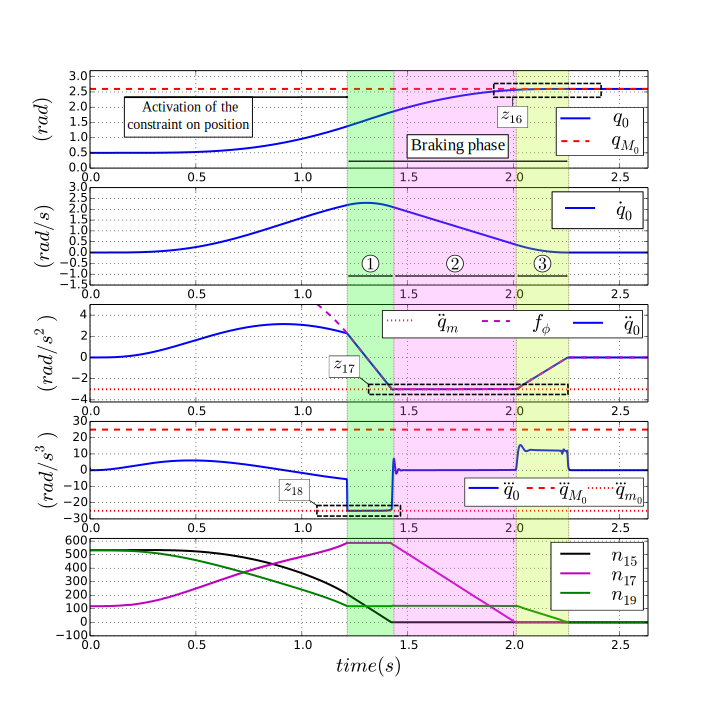
\includegraphics[width=1.05\columnwidth]{figures/11_Posi_constr_jerk_acc_comp_complete_formula_3}} 
%%\end{center}
%\end{frame}
%
%
%
%
%
%
%
%
%
%
%
%
%
%
%\begin{frame}
%\frametitle{{\textcolor{white}{Incompatibility case related to the constraint on articular position $\vect{q}$} -- Results}}
%\begin{center}
%{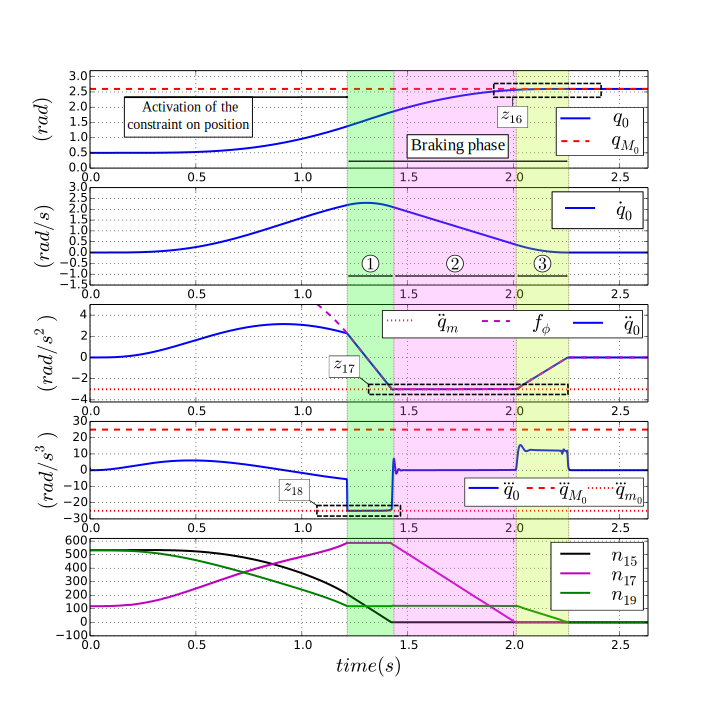
\includegraphics[width=0.75\columnwidth]{figures/11_Posi_constr_jerk_acc_comp_complete_formula_3}} 
%\end{center}
%\end{frame}







%%%%%%%%%%%%%%%%%%%%%%%%%%%%%%%%ù


%\begin{frame}
%\frametitle{{\textcolor{white}{Incompatibility case related to the constraint on articular velocity $\vect{\dot{q}}$}}}
%
%$\bullet$ \textcolor{red}{\textbf{Naive}} formulation of the constraint on $\vect{\dot{q}}$:
%\begin{subequations}
%\label{eq:const_1_literature}
%\begin{empheq}[left={}\empheqlbrace]{align}
%\frac{1}{\textcolor{blue}{\delta t}} (\vect{\textcolor{blue-violet}{\dot{q}_{m}}}-\vect{\dot{q}}_{|k}) &\leq \textcolor{red}{\vect{\ddot{q}}_{|k}^{c}} \leq \frac{1}{\textcolor{blue}{\delta t}} (\vect{\textcolor{blue-violet}{\dot{q}_{M}}}-\vect{\dot{q}}_{|k}),  \label{eq:cnt_lit_11251}\\
%\textcolor{blue-violet}{\vect{\dddot{q}}_{m}} \textcolor{blue}{\delta t}+\vect{\ddot{q}}_{|k} &\leq \textcolor{red}{\vect{\ddot{q}}_{|k}^{c}} \leq \textcolor{blue-violet}{\vect{\dddot{q}}_{M}} \textcolor{blue}{\delta t}+\vect{\ddot{q}}_{|k}. \label{eq:cnt_lit_32533}
%\end{empheq}
%\end{subequations}
%\hspace{3mm}\rightarrow \textcolor{red}{\textbf{No optimal solution is available for the control problem.}} \\
%\vspace{10mm}
%$\bullet$ \textcolor{red}{\textbf{New}} formulation of the constraint $\vect{\dot{q}}$:
%\begin{subequations}
%\label{eq:const_1_literature}
%\begin{empheq}[left={}\empheqlbrace]{align}
%f_{\beta}(\dot{q}_{|k}, \textcolor{blue-violet}{\dot{q}_m}, \textcolor{blue-violet}{\dddot{q}_M}, \textcolor{blue}{n_2}) &\leq \textcolor{red}{\vect{\ddot{q}}_{|k}^{c}} \leq f_{\alpha}(\dot{q}_{|k}, \textcolor{blue-violet}{\dot{q}_M}, \textcolor{blue-violet}{\dddot{q}_m}, \textcolor{blue}{n_1}),  \label{eq:cnt_lit_112rg51}\\
%\textcolor{blue-violet}{\vect{\dddot{q}}_{m}} \textcolor{blue}{\delta t}+\vect{\ddot{q}}_{|k} &\leq \textcolor{red}{\vect{\ddot{q}}_{|k}^{c}} \leq \textcolor{blue-violet}{\vect{\dddot{q}}_{M}} \textcolor{blue}{\delta t}+\vect{\ddot{q}}_{|k}. \label{eq:cnt_lit_325rfgrg33}
%\end{empheq}
%\end{subequations}
%\hspace{3mm}{\small \rightarrow \textcolor{ao(english)}{\textbf{No problem of constraints incompatibility, an optimal solution is guaranteed.}} }
%\end{frame}











\begin{frame}
\frametitle{{\textcolor{white}{Constraint on articular velocity: naive \textit{VS} new formulation}}}

\hspace{-5mm}
$\bullet$ \textcolor{black}{\textbf{Naive formulation}}:
\begin{equation}
\vect{\dot{q}}_{|k{\color{blue}+1}}  =  \vect{\dot{q}}_{|k} + {\color{blue}\delta t} {\color{red}\vect{\ddot{q}}_{|k}^c} \leq \vect{\dot{q}}_{M},
\end{equation}

\setbeamertemplate{itemize items}[triangle]
\begin{itemize}
\addtolength{\itemindent}{-2mm}
\item Discretization over only {\color{blue}one $\delta t$} time-step. 
\setlength\itemsep{-0.2em}
\item Accounts only for the system's state $\vect{\dot{q}}_{|k}$ \textbf{{\color{red}and not}} for its producible jerk {\color{blue-violet}$\vect{\dddot{q}}_{m}$}.
\end{itemize}

\vspace{1mm}
\begin{itemize}
\addtolength{\itemindent}{-1mm}
\item[\hookrightarrow] \fbox{\begin{minipage}{15em}{                   
{\color{red}\textbf{Often results in incompatibility !}}
}
\end{minipage}}
\end{itemize}
\vspace{8mm}


\only<2>{
\hspace{-5mm}
$\bullet$ {\color{blue}\textbf{New proposed formulation}}:
\begin{equation}
\dot{q}_{|k+{\color{blue}n_1}} = \dot{q}_{|k} + {\color{blue}n_1} {\color{red}\ddot{q}_{|k}^c} {\color{blue}\delta t} + \frac{({\color{blue}n_1}^2-{\color{blue}n_1})}{2} {\color{blue-violet}\dddot{q}_{m}} {\color{blue}\delta t}^2 \leq \vect{\dot{q}}_{M},
\end{equation}

\setbeamertemplate{itemize items}[triangle]
\begin{itemize}
\addtolength{\itemindent}{3mm}
\item Discretization over {\color{blue} $n_1 \delta t$} time-steps. 
\setlength\itemsep{-0.2em}
\item Accounts for both the system's state $\vect{\dot{q}}_{|k}$ \textbf{{\color{ao(english)}and}} for its producible jerk {\color{blue-violet}$\vect{\dddot{q}}_{m}$}.
\end{itemize}

\vspace{1mm}
\begin{itemize}
\addtolength{\itemindent}{-1mm}
\item[\hookrightarrow] \fbox{\begin{minipage}{22em}{                   
{\color{ao(english)}\textbf{No incompatibility with the constraint on jerk !}}
}
\end{minipage}}
\end{itemize}




}
\end{frame}







%$\bullet$ \textcolor{armygreen}{\textbf{Solution: the constraints on $\vect{q}$ and $\dot{q}$ must be reformulated:}}

%\begin{frame}
%\frametitle{{\textcolor{white}{New Formulation of the Constraint on Articular Velocity $\vect{\dot{q}}$}}}
%$\bullet$ \textcolor{red}{\textbf{Braking phase}} for a joint coping with a velocity limit $\vect{\dot{q}}_M \geq 0$:
%\begin{equation} 
%\begin{split}
%\textit{S}_{|k+1}&\left\{\begin{array}{lcl}
%\vspace{1mm}
%\dot{q}_{|k+1} \hspace{1mm}= \dot{q}_{|k} + \ddot{q}_{|k} \delta t, \\
%\ddot{q}_{|k+1} \hspace{1mm}= \ddot{q}_{|k} + \textcolor{red}{\dddot{q}_{m}} \delta t.
%\end{array}\right.\\
%\textit{S}_{|k+2}&\left\{\begin{array}{lcl}
%\vspace{1mm}
%\dot{q}_{|k+2} \hspace{1mm}= \dot{q}_{|k+1} + \ddot{q}_{|k+1} \delta t, \\
%\ddot{q}_{|k+2} \hspace{1mm}= \ddot{q}_{|k+1} + \textcolor{red}{\dddot{q}_{m}} \delta t.
%\end{array}\right.\\
%& \hspace{7mm}\vdots\ \hspace{12mm}\vdots\\\
%\textit{S}_{|k+\textcolor{blue-violet}{n_{1}}}&\left\{\begin{array}{lcl}
%\vspace{1mm}
%\dot{q}_{|k+\textcolor{blue-violet}{n_{1}}} = \dot{q}_{|k+\textcolor{blue-violet}{n_{1}}-1} + \ddot{q}_{|k+\textcolor{blue-violet}{n_{1}}-1} \delta t, \\
%\ddot{q}_{|k+\textcolor{blue-violet}{n_{1}}} = \ddot{q}_{|k+\textcolor{blue-violet}{n_{1}}-1} + \textcolor{red}{\dddot{q}_{m}} \delta t.
%\end{array}\right.
%\end{split}
%\label{eq:discretized_dynamics_vel}
%\end{equation} \vspace{4mm}
%
%$\bullet$ The \textcolor{red}{\textbf{New Formulation}} of the Articular Velocity Constraint is of the Form:
%\begin{equation}
%\textcolor{red}{\ddot{q}_{|k}^{c}} \leq f_{\alpha}(\dot{q}_{|k}, \textcolor{red}{\dot{q}_M}, \textcolor{red}{\dddot{q}_m}, \textcolor{blue-violet}{n_1}) 
%\Longleftrightarrow \textcolor{red}{\ddot{q}_{|k}^{c}} \leq \frac{(\textcolor{red}{\dot{q}_M}-\dot{q}_{|k})}{\textcolor{blue-violet}{n_1} \delta t} - \frac{(\textcolor{blue-violet}{n_1}-1)}{2} \textcolor{red}{\dddot{q}_m} \delta t. 
%\label{eq:q_ddot_vel_jerk_comp_aa_n1}
%\end{equation}
%\end{frame}






\begin{frame}
\frametitle{{\textcolor{white}{Constraint on articular velocity: naive \textit{VS} new formulation} -- Results}}
$\bullet$ \textbf{Naive formulation:} \hspace{27mm} $\bullet$ {\color{blue}\textbf{New formulation:}}
\begin{columns}
\column{.45\textwidth}
\vspace{2mm}

{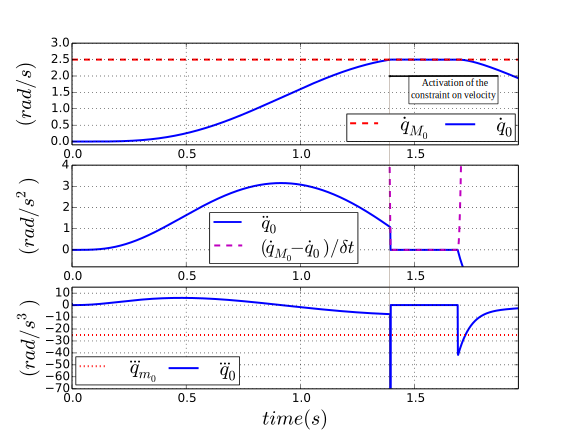
\includegraphics[width=0.91\columnwidth]{figures/0_Vel_constr_classic}} 


\begin{itemize}
\addtolength{\itemindent}{-1mm}
\item[\hookrightarrow] \fbox{\begin{minipage}{9.5em}{                   
\textbf{$\bullet${\color{red}High peak of jerk !}} \\
\textbf{$\bullet${\color{red}If}} $\vect{\dddot{q}}$ \textbf{{\color{red}constrained, the control problem is unsolvable.}}
}

\end{minipage}}
\end{itemize}



\vspace{-10mm}
\column{.55\textwidth}

\end{columns}
\end{frame}













\begin{frame}[noframenumbering]
\frametitle{{\textcolor{white}{Constraint on articular velocity: naive \textit{VS} new formulation} -- Results}}
$\bullet$ \textbf{Naive formulation:} \hspace{27mm} $\bullet$ {\color{blue}\textbf{New formulation:}}
\begin{columns}
\column{.45\textwidth}
\vspace{2mm}

{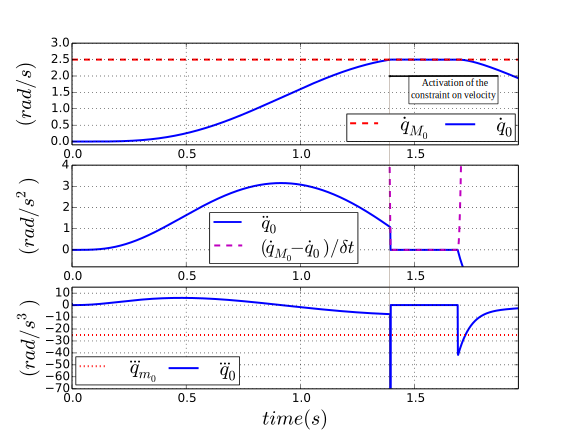
\includegraphics[width=0.91\columnwidth]{figures/0_Vel_constr_classic}} 


\begin{itemize}
\addtolength{\itemindent}{-1mm}
\item[\hookrightarrow] \fbox{\begin{minipage}{9.5em}{                   
\textbf{$\bullet${\color{red}High peak of jerk !}} \\
\textbf{$\bullet${\color{red}If}} $\vect{\dddot{q}}$ \textbf{{\color{red}constrained, the control problem is unsolvable.}}
}

\end{minipage}}
\end{itemize}



\vspace{-10mm}
\column{.55\textwidth}
\vspace{2mm}

{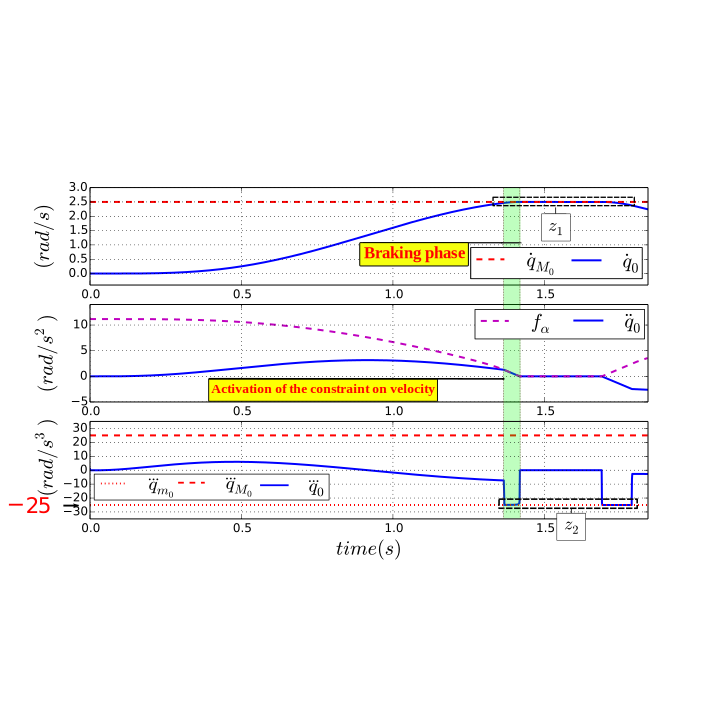
\includegraphics[width=1.01\columnwidth]{figures/1_Vel_constr_jerk_comp_}} 


\begin{itemize}
\addtolength{\itemindent}{0mm}
\item[\hookrightarrow] \fbox{\begin{minipage}{13em}{                   
\textbf{$\bullet${\color{ao(english)}Both jerk and velocity limits are satisfied.}}
}
\end{minipage}}
\end{itemize}
\end{columns}
\end{frame}







%%%%%PEUT ETRE A REMETTRE
%\begin{frame}
%\frametitle{{\textcolor{white}{Final bounds on the acceleration control variable $\textcolor{white}{\vect{\ddot{q}}_{|k}^{c}}$}}}
%\textbf{\textcolor{carmine}{Final}} bounds on $\textcolor{red}{\vect{\ddot{q}}_{|k}^{c}}$ that accounts for all the articular constraints :
%\resizebox{1.05\hsize}{!}{%
%\begin{equation}
%f_{\omega}(\textcolor{blue-violet}{q_m}, \textcolor{blue-violet}{\dot{q}_m}, \textcolor{blue-violet}{\ddot{q}_m}, \textcolor{blue-violet}{\dddot{q}_{m}}, \textcolor{blue-violet}{\ddot{q}_M}, \textcolor{blue-violet}{\dddot{q}_M}, \textcolor{blue-violet}{\dddot{q}_m})  \leq \textcolor{red}{\vect{\ddot{q}}_{|k}^{c}} \leq f_{\psi}(\textcolor{blue-violet}{q_M}, \textcolor{blue-violet}{\dot{q}_M}, \textcolor{blue-violet}{\ddot{q}_M}, \textcolor{blue-violet}{\dddot{q}_{M}}, \textcolor{blue-violet}{\ddot{q}_m}, \textcolor{blue-violet}{\dddot{q}_m}, \textcolor{blue-violet}{\dddot{q}_M}).
%\label{eq:qddot_FINAL_CONSTR_1_final}
%\end{equation}
%}
%\begin{center}
%{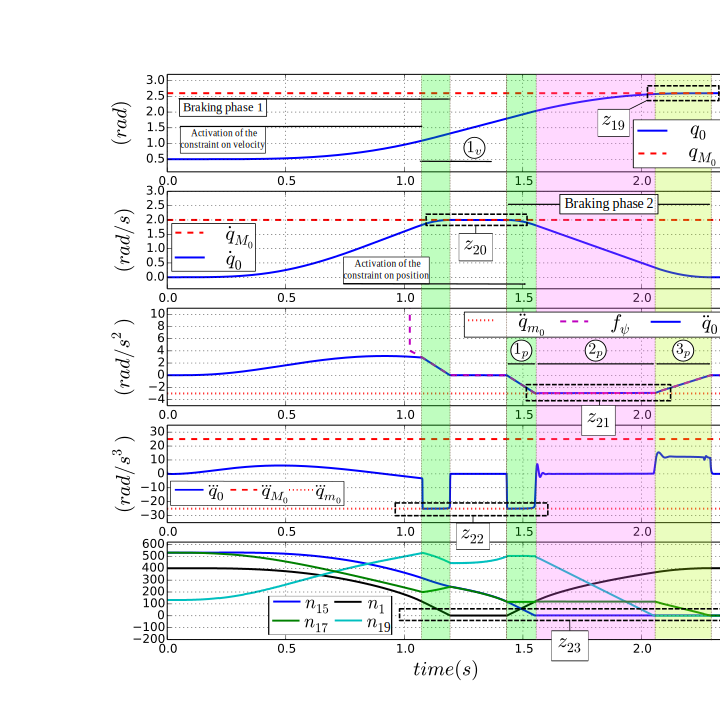
\includegraphics[width=0.7\columnwidth]{figures/12_all_constr}} 
%\end{center}
%\end{frame}


%\begin{frame}
%\frametitle{{\textcolor{white}{Final bounds on the acceleration control variable $\vect{\ddot{q}}_{|k}^{c}$} -- Results}}
%\begin{center}
%{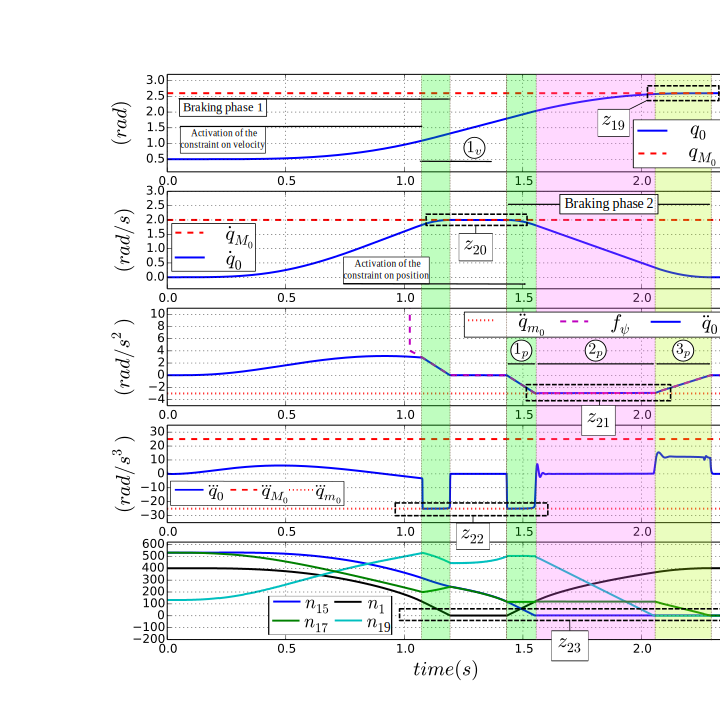
\includegraphics[width=0.75\columnwidth]{figures/12_all_constr}} 
%\end{center}
%\end{frame}




\subsection{Conclusion I}
\begin{frame}
\frametitle{{\textcolor{white}{Conclusion I}}}
\setbeamertemplate{itemize items}[triangle]
\begin{itemize}
\item With the \textcolor{napiergreen}{\textbf{new introduced formulations}}, the articular constraints: 
\begin{subequations}
\label{eq:const_1_literature}
\begin{empheq}[left={}\empheqlbrace]{align}
\vect{q}_{m} & \leq \vect{q}\hspace{2mm}\leq \vect{q}_{M},\label{eq:cnt_lit_1}\\
\vect{\dot{q}}_{m} & \leq \vect{\dot{q}}\hspace{2mm}\leq \vect{\dot{q}}_{M},\label{eq:cnt_lit_2}\\    
{\color{blue-violet}\vect{\ddot{q}}_{m}} & \leq \textcolor{red}{\vect{\ddot{q}}_{|k}^{c}}\leq {\color{blue-violet}\vect{\ddot{q}}_{M}},\label{eq:cnt_lit_3}\\
{\color{blue-violet}\vect{\dddot{q}}_{m}}  & \leq \vect{\dddot{q}}\hspace{2mm}\leq {\color{blue-violet}\vect{\dddot{q}}_{M}}.\label{eq:cnt_lit_5}
\end{empheq}
\end{subequations}
\end{itemize}
\vspace{1mm}
\begin{itemize}
\addtolength{\itemindent}{0mm}
\item[\hookrightarrow] \fbox{\begin{minipage}{22em}{                   
{\color{red}\textbf{Are all simultaneously and reactively coped with.}}
}
\end{minipage}}
\end{itemize}




\begin{itemize}
\addtolength{\itemindent}{0mm}
\item[\hookrightarrow] \fbox{\begin{minipage}{30em}{                   
\textcolor{blue}{\textbf{The viability of the state of the system}} \textcolor{blue}{\textbf{is guaranteed over an infinite horizon of time.}}
}
\end{minipage}}
\end{itemize}


%\item \textcolor{red}{\textbf{An optimal control solution}} \textcolor{red}{\textbf{is guaranteed}} over an infinite horizon of time.
%\vspace{5mm}
%
%\item This optimal solution allows \textcolor{blue}{\textbf{coping simultaneously}} \textcolor{blue}{\textbf{with all}} the considered \textcolor{blue}{\textbf{constraints}}. 

\end{frame}









\begin{frame}
%\frametitle{{\textcolor{white}{\hspace{0.3cm}Complexity of Problem 1
%}}}
\frametitle{{\textcolor{white}{\hspace{0.3cm}Conclusion I
}}}
$\bullet$ {\color{red}\textbf{Even more complex}}
\begin{figure}[!ht]
\centering
\includegraphics[width=1.0\linewidth]{figures/car_example_14}
%\caption{Braking phase for the car in scenario 1 as it stops before hitting the wall.}
%\label{fig:car_example_14}
\end{figure}
$\bullet$ \textbf{Solving the problem of constraints incompatibility \textcolor{red}{is more complex} if:}
\begin{itemize}
\addtolength{\itemindent}{5mm}
\item[1.] The position of the obstacle is dynamic \textcolor{red}{$\widetilde{d}_{safe}$}.
\item[2.] The car's deceleration capability \textcolor{red}{$-\widetilde{a}_{Max}$} is variable.
\end{itemize}  
\vspace{5mm}
\end{frame}










\begin{frame}
%\frametitle{{\textcolor{white}{\hspace{0.3cm}Complexity of Problem 1
%}}}
\frametitle{{\textcolor{white}{\hspace{0.3cm}Conclusion I
}}}
\hspace{-8mm}
$\bullet$ {\color{blue}\textbf{The robot system's articular deceleration capabilities are not constant:}}

\begin{columns}
\column{\paperwidth-20mm}


\begin{equation}
M(\vect{q}_{|k}) \textcolor{red}{\vect{\ddot{q}}_{|k}^{c}} + \vect{b}(\vect{q}_{|k},\vect{\dot{q}}_{|k}) = \textcolor{red}{\vect{\tau}_{|k}^{c}},
\label{eq:dyn_eq}
\end{equation} \\

\begin{columns}
\column{.5\paperwidth}
\hspace{-30mm}
\begin{subequations}
\label{eq:const_1_literature}
\begin{empheq}[left={}\empheqlbrace]{align}
\vect{q}_{m} & \leq \vect{q}\hspace{2mm}\leq \vect{q}_{M},\label{eq:cnt_lit_1}\\
\vect{\dot{q}}_{m} & \leq \vect{\dot{q}}\hspace{2mm}\leq \vect{\dot{q}}_{M},\label{eq:cnt_lit_2}\\    
{\color{blue-violet}\vect{\ddot{q}}_{m}} & \leq \textcolor{red}{\vect{\ddot{q}}_{|k}^{c}}\leq {\color{blue-violet}\vect{\ddot{q}}_{M}}, \hspace{1mm}({\color{blue-violet}\vect{\tau}_{m}} \leq \textcolor{red}{\vect{\tau}_{|k}^{c}} \leq {\color{blue-violet}\vect{\tau}_{M}})\label{eq:cnt_lit_3}\\
{\color{blue-violet}\vect{\dddot{q}}_{m}}  & \leq \vect{\dddot{q}}\hspace{2mm}\leq {\color{blue-violet}\vect{\dddot{q}}_{M}}.\label{eq:cnt_lit_5}
\end{empheq}
\end{subequations}


\column{.5\paperwidth}
\hspace{1mm}
\fbox{\begin{minipage}{12.9em}{
$\bullet$ {\color{blue-violet}$\vect{\tau}_{M}$} {\color{red}and} {\color{blue-violet}$\vect{\tau}_{m}$} {\color{red}are constant.}\\                   
$\bullet$ {\color{blue-violet}$\vect{\ddot{q}}_M$}{\color{red}}{\color{red},} {\color{blue-violet}$\vect{\ddot{q}}_m$}{\color{red},} {\color{blue-violet}$\vect{\dddot{q}}_M$}{\color{red}}{\color{red},} {\color{red}and} {\color{blue-violet}$\vect{\dddot{q}}_m$} {\color{red}are} \\ {\color{white}iiii}{\color{red}configuration dependent.}
%\bullet \hspace{1mm} {\color{red}To simplify,} {\color{blue-violet}$\vect{\ddot{q}}_M$} {\color{red}and} {\color{blue-violet}$\vect{\ddot{q}}_m$} {\color{red}are considered constant.}
}
\end{minipage}}
\end{columns}





\vspace{5mm}

\begin{columns}
\column{.55\paperwidth}

\begin{center}
\vspace{-13mm}
\hspace{-5mm}
\only<1>{\movie[showcontrols=true,autostart=true,loop=true]{\includegraphics[width=0.6\textwidth]{videos/constr_comp.png}}{videos/constr_com-5.mp4}}
\end{center}

\column{.45\paperwidth}
\hspace{-5mm}
\vspace{5mm}
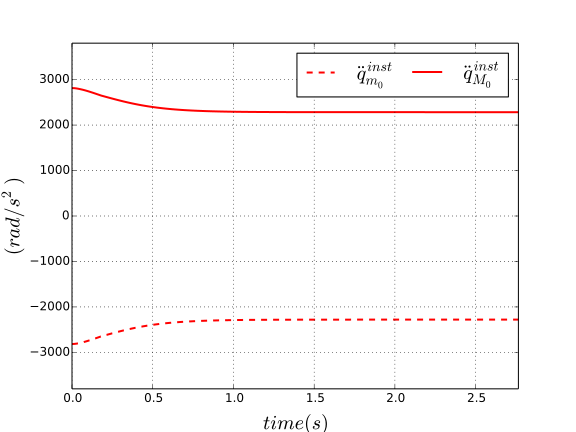
\includegraphics[width=0.80\columnwidth]{figures/instant_articular_acceleration_capability.pdf}
\end{columns}

\vspace{-3mm}

$\bullet$ {\color{blue}\textbf{Open problem:} constraints incompatibility for dynamic constraints, use MPC ?}
\end{columns}



\end{frame}










%\begin{frame}
%\frametitle{Outline}
%  \tableofcontents
%\end{frame}
%





%\begin{frame}
%\frametitle{Outline}
%  \tableofcontents
%\end{frame}




%%A REMETTRE ??????????????????
%\begin{frame}
%\frametitle{{\textcolor{white}{\hspace{0.3cm}Constraints Incompatibility when Controlling Robots}}}
%\begin{itemize}
%\item[I.] \textbf{Constraints expressed in Cartesian space:}
%\begin{figure}[!ht]
%\centering
%\includegraphics[width=0.7\linewidth]{\figurepath/car_example_2}
%\caption{Braking phase for the car in scenario 1 as it stops before hitting the wall.}
%\label{fig:car_example_2}
%\end{figure}
%
%\item[II.] \textbf{Constraints expressed in Articular space:}
%\end{itemize} 
%\begin{figure}[!ht]
%\centering
%\includegraphics[width=0.7\linewidth]{\figurepath/car_example_2}
%\caption{Braking phase for the car in scenario 1 as it stops before hitting the wall.}
%\label{fig:car_example_2}
%\end{figure}
%\end{frame}





%\subsection{Constraints incompatibility on a reactively controlled robotic arm.}
%\begin{frame}
%\frametitle{{\textcolor{white}{\hspace{0.2cm}Reactively controlled KUKA LWR4}}}
%\begin{center}
%\only<1>{\movie[showcontrols=true,autostart=true]{\includegraphics[width=0.8\textwidth]{videos/constr_comp.png}}{videos/constr_com-5.mp4}}
%\end{center}
%\end{frame}










%
%\subsection{Conclusion I}
%\begin{frame}
%\frametitle{{\textcolor{white}{Conclusion I}}}
%\begin{itemize}
%\item Using the \textcolor{napiergreen}{\textbf{new introduced formulations}} of the robot's articular constraints, \textcolor{napiergreen}{\textbf{the problem of constraints incompatibility is resolved}}.
%\vspace{5mm}
%\item \textcolor{red}{\textbf{An optimal solution}} to the control problem \textcolor{red}{\textbf{is guaranteed}} at every control time-step.
%\vspace{5mm}
%\item This optimal solution allows \textcolor{blue}{\textbf{coping simultaneously}} \textcolor{blue}{\textbf{with all}} the considered \textcolor{blue}{\textbf{constraints}}. 
%\end{itemize}
%\end{frame}


%PEUT ETRE A REMETTRE
%\section{Part II: Safe Human-Robot Interaction}
%\begin{frame}
%\frametitle{{\textcolor{white}{\hspace{0.3cm}Part II: Safe Human-Robot Interaction}}}
%\begin{center}     
%{\fontsize{15}{40}\selectfont {\color{violet}\textbf{Part II:}} \textbf{Safe Human-Robot Interaction.}}
%\end{center}             
%\end{frame}







%%%%%%%%%%%%%%%%%%%%%%%%%%%%%%%%%%%%%%ù
\begin{frame}
\frametitle{{\textcolor{white}{\hspace{0.3cm}Safety}}}


\begin{columns}

\column{.90\paperwidth}

\begin{center}                
\includegraphics[width=0.55\textwidth ]{figures/7.pdf}
\end{center}       

\end{columns}


\begin{itemize}
\item[\hookrightarrow] \fbox{\begin{minipage}{30.4em}{ \textbf{Dimensions addressed in our work:}
\setbeamertemplate{itemize items}[triangle]  
\addtolength{\itemindent}{-3mm}                  
\begin{itemize}
\item[\textbf{I.}] {\color{red}\transparent{0.4}\textbf{Problems related to the use of reactive control loops.}}
\item[\textbf{II.}] {\color{red}\transparent{1.0}\textbf{Safety during Human-Robot physical Interaction.}} %
\end{itemize}}
\end{minipage}}
\end{itemize}
%\hbox{\color{red}\transparent{0.1} MY THESIS}

\end{frame}
%%%%%%%%%%%%%%%%%%%%%%%%%%%%%%%%%%%%%%%%









%\begin{frame}
%\frametitle{Outline}
%  \tableofcontents
%\end{frame}





\section{Part II: Safe Human-Robot Interaction}
%%%%%%%%%%%%%%%%%%%%%%%%%%%%%%%%%%%%%%ù
\begin{frame}
  \frametitle{{\textcolor{white}{\hspace{0.3cm}Safety during Human-Robot Interaction -- state of the art}}}
  
 \vspace{-3mm} 
\begin{columns}
\column{.47\paperwidth}
\vspace{-5mm}
\begin{center}
\vspace{2mm}
\includegraphics[width=0.4\textwidth ]{figures/Human_robot_int.png}
\end{center}
 \vspace{-3mm} 
\column{.47\paperwidth}
$\bullet$ \textbf{Motivations:}                     
\begin{center}
\setbeamertemplate{itemize items}[triangle]                        
\begin{itemize}
\item Safely share the robot's workspace.
\item Enable safe Human-Robot physical Interaction.
\end{itemize}                                            
\end{center}
\end{columns}

\vspace{7mm}
\hspace{-4mm}
$\bullet$ \textbf{State of the art: safety at the control level}
\vspace{6mm}
\includegraphics[width=1.0\textwidth]{figures/sttt0.pdf}
\vspace{-1mm}






\end{frame}
%%%%%%%%%%%%%%%%%%%%%%%%%%%%%%%%%%%%%%%%














%%%%%%%%%%%%%%%%%%%%%%%%%%%%%%%%%%%%%%ù
\begin{frame}[noframenumbering]
  \frametitle{{\textcolor{white}{\hspace{0.3cm}Safety during Human-Robot Interaction -- state of the art}}}
  
 \vspace{-3mm} 
\begin{columns}
\column{.47\paperwidth}
\vspace{-5mm}
\begin{center}
\vspace{2mm}
\includegraphics[width=0.4\textwidth ]{figures/Human_robot_int.png}
\end{center}
 \vspace{-3mm} 
\column{.47\paperwidth}
$\bullet$ \textbf{Motivations:}                     
\begin{center}
\setbeamertemplate{itemize items}[triangle]                        
\begin{itemize}
\item Safely share the robot's workspace.
\item Enable safe Human-Robot physical Interaction.
\end{itemize}                                            
\end{center}
\end{columns}

\vspace{7mm}
\hspace{-4mm}
$\bullet$ \textbf{State of the art: safety at the control level}
\vspace{6mm}
\includegraphics[width=1.0\textwidth]{figures/sttt1.pdf}
\vspace{-1mm}






\end{frame}
%%%%%%%%%%%%%%%%%%%%%%%%%%%%%%%%%%%%%%%%



%%%%%%%%%%%%%%%%%%%%%%%%%%%%%%%%%%%%%%ù
\begin{frame}[noframenumbering]
  \frametitle{{\textcolor{white}{\hspace{0.3cm}Safety during Human-Robot Interaction -- state of the art}}}
  
 \vspace{-3mm} 
\begin{columns}
\column{.47\paperwidth}
\vspace{-5mm}
\begin{center}
\vspace{2mm}
\includegraphics[width=0.4\textwidth ]{figures/Human_robot_int.png}
\end{center}
 \vspace{-3mm} 
\column{.47\paperwidth}
$\bullet$ \textbf{Motivations:}                     
\begin{center}
\setbeamertemplate{itemize items}[triangle]                        
\begin{itemize}
\item Safely share the robot's workspace.
\item Enable safe Human-Robot physical Interaction.
\end{itemize}                                            
\end{center}
\end{columns}

\vspace{7mm}
\hspace{-4mm}
$\bullet$ \textbf{State of the art: safety at the control level}
\vspace{6mm}
\includegraphics[width=1.0\textwidth]{figures/sttt2.pdf}
\vspace{-1mm}






\end{frame}
%%%%%%%%%%%%%%%%%%%%%%%%%%%%%%%%%%%%%%%%




%%%%%%%%%%%%%%%%%%%%%%%%%%%%%%%%%%%%%%ù
\begin{frame}[noframenumbering]
  \frametitle{{\textcolor{white}{\hspace{0.3cm}Safety during Human-Robot Interaction -- state of the art}}}
  
 \vspace{-3mm} 
\begin{columns}
\column{.47\paperwidth}
\vspace{-5mm}
\begin{center}
\vspace{2mm}
\includegraphics[width=0.4\textwidth ]{figures/Human_robot_int.png}
\end{center}
 \vspace{-3mm} 
\column{.47\paperwidth}
$\bullet$ \textbf{Motivations:}                     
\begin{center}
\setbeamertemplate{itemize items}[triangle]                        
\begin{itemize}
\item Safely share the robot's workspace.
\item Enable safe Human-Robot physical Interaction.
\end{itemize}                                            
\end{center}
\end{columns}

\vspace{7mm}
\hspace{-4mm}
$\bullet$ \textbf{State of the art: safety at the control level}
\vspace{6mm}
\includegraphics[width=1.0\textwidth]{figures/sttt3.pdf}
\vspace{-1mm}






\end{frame}
%%%%%%%%%%%%%%%%%%%%%%%%%%%%%%%%%%%%%%%%




%%%%%%%%%%%%%%%%%%%%%%%%%%%%%%%%%%%%%%ù
\begin{frame}[noframenumbering]
  \frametitle{{\textcolor{white}{\hspace{0.3cm}Safety during Human-Robot Interaction -- state of the art}}}
  
 \vspace{-3mm} 
\begin{columns}
\column{.47\paperwidth}
\vspace{-5mm}
\begin{center}
\vspace{2mm}
\includegraphics[width=0.4\textwidth ]{figures/Human_robot_int.png}
\end{center}
 \vspace{-3mm} 
\column{.47\paperwidth}
$\bullet$ \textbf{Motivations:}                     
\begin{center}
\setbeamertemplate{itemize items}[triangle]                        
\begin{itemize}
\item Safely share the robot's workspace.
\item Enable safe Human-Robot physical Interaction.
\end{itemize}                                            
\end{center}
\end{columns}

\vspace{7mm}
\hspace{-4mm}
$\bullet$ \textbf{State of the art: safety at the control level}
\vspace{6mm}
\includegraphics[width=1.0\textwidth]{figures/sttt4.pdf}
\vspace{-1mm}






\end{frame}
%%%%%%%%%%%%%%%%%%%%%%%%%%%%%%%%%%%%%%%%



%%%%%%%%%%%%%%%%%%%%%%%%%%%%%%%%%%%%%%ù
\begin{frame}[noframenumbering]
  \frametitle{{\textcolor{white}{\hspace{0.3cm}Safety during Human-Robot Interaction -- state of the art}}}
  
 \vspace{-3mm} 
\begin{columns}
\column{.47\paperwidth}
\vspace{-5mm}
\begin{center}
\vspace{2mm}
\includegraphics[width=0.4\textwidth ]{figures/Human_robot_int.png}
\end{center}
 \vspace{-3mm} 
\column{.47\paperwidth}
$\bullet$ \textbf{Motivations:}                     
\begin{center}
\setbeamertemplate{itemize items}[triangle]                        
\begin{itemize}
\item Safely share the robot's workspace.
\item Enable safe Human-Robot physical Interaction.
\end{itemize}                                            
\end{center}
\end{columns}

\vspace{7mm}
\hspace{-4mm}
$\bullet$ \textbf{State of the art: safety at the control level}
\vspace{6mm}
\includegraphics[width=1.0\textwidth]{figures/sttt.pdf}
\vspace{-1mm}

\begin{columns}
\column{\paperwidth-22pt}


\only<2-3>{\begin{itemize}
\addtolength{\itemindent}{2mm}
\item[\hookrightarrow] \fbox{\begin{minipage}{20.4em}{                   
{\color{red}\textbf{Available approaches not sufficiently generic.}}
}
\end{minipage}}
\end{itemize}}
\vspace{-2mm}
\only<3>{\begin{itemize}
\addtolength{\itemindent}{2mm}
\item[\hookrightarrow] \fbox{\begin{minipage}{28.6em}{                   
{\color{ao(english)}\textbf{Contribution II: the use of energy as a safety indicator to modulate the system's dynamics.}}
}
\end{minipage}}
\end{itemize}}



\end{columns}



\end{frame}
%%%%%%%%%%%%%%%%%%%%%%%%%%%%%%%%%%%%%%%%








%%%%%%%%%%%%%%%%%%%%%%%%%%%%%%%% 1 %%%%%%%%%%%%%%%%%%%%%%%%%%%%%%%%%%%%%%%%
%\begin{frame}
%\frametitle{{\textcolor{white}{\hspace{0.3cm}Motivation}}}
%
%\begin{center}
%\includegraphics[width=0.45\textwidth]{figures/Human_robot_int.png}
%\end{center}      
%%\item Ensure the safety of the human operator during human-robot interaction.
%$\bullet$ \textbf{Motivations:} 
%\setbeamertemplate{itemize items}[triangle]
%\begin{itemize}
%\item Safely share the robot's workspace.
%\item Enable safe human-robot physical interaction
%\end{itemize}
%
%$\bullet$ \textbf{Safety indicators/parameters in the existing literature:} 
%\setbeamertemplate{itemize items}[triangle]
%
%\begin{itemize}
%\item Velocity, Inertia,  Impact forces and Contact forces. 
%\end{itemize}
%
%\textbf{Proposed safety indicators:}  
%\setbeamertemplate{itemize items}[triangle]
%\begin{itemize}
%\item The robot's \textbf{{\color{blue} \underline{Kinetic}}} and {\color{blue} \textbf{\underline{Potential energy}}}           
%\end{itemize}             
%\end{frame}
%%%%%%%%%%%%%%%%%%%%%%%%%%%%%%%% 1 %%%%%%%%%%%%%%%%%%%%%%%%%%%%%%%%%%%%%%%%
%
%
%
%
%
%
%
%%%%%%%%%%%%%%%%%%%%%%%%%%%%%%%%%%%%%%%ù
%\begin{frame}
%\frametitle{{\textcolor{white}{\hspace{0.3cm}Collaborative robotics}}}
%
%
%\begin{columns}
%
%
%
%\column{.47\paperwidth}
%%                \begin{tcolorbox}[colback=white,title=Frictional non-rigid contact]
%\begin{center}                
%\includegraphics[width=\textwidth ]{figures/robots.pdf}
%\end{center}                  
%
%%                \end{tcolorbox}
%
%\column{.47\paperwidth}
%
%Many aspects are to be considered:
%\setbeamertemplate{itemize items}[triangle]                    
%\begin{itemize}
%\addtolength{\itemindent}{-6mm}
%\item \textbf{Safety}: the robot is forbidden from compromising the physical integrity of the human.
%\item \textbf{Cognitive aspects}: can significantly enhance the quality of the interaction.
%\item \textbf{Reactive control}: as offline planning is not adapted for dynamic/unknown environments.
%\item \textbf{Hardware design}: must be modified as rigid and heavy structures are not adapted for Human-Robot physical interaction.
%\item Perception and sensing: when intracting.
%
%
%\item Lightweight structures using fiber reinforced \\ \hspace{-7mm} composite materials.
%\setlength\itemsep{1em}
%\item Redundant joint position sensors to emulate \\ \hspace{-7mm} compliance.
%\setlength\itemsep{1em}
%\item Torque sensors. 
%\setlength\itemsep{1em}
%\item[\hookrightarrow] \textbf{More suitable for human-robot physical} \\ \hspace{-7mm} \textbf{interaction}.
%\end{itemize}
%
%\end{columns}
%\vspace{5mm}
%
%\setbeamertemplate{itemize items}[triangle]                        
%\begin{itemize}
%\item {\color{red}\textbf{When reactive control loops are used:}}
%%\setlength\itemsep{2em}
%\item[\hookrightarrow] No optimal control solution can be guaranteed.
%%\setlength\itemsep{1em}
%\item[\hookrightarrow] Possible constraints violation.
%%\setlength\itemsep{1em}
%\item[\hookrightarrow] Safety for the robotic system and its environment can be compromised.
%\end{itemize}
%
%\end{frame}
%%%%%%%%%%%%%%%%%%%%%%%%%%%%%%%%%%%%%%%%%
%
%
%
%
%
%
%
%%%%%%%%%%%%%%%%%%%%%%%%%%%%%%%%%%%%%%%ù
%\begin{frame}
%\frametitle{{\textcolor{white}{\hspace{0.3cm}Reactive control of collaborative robots}}}
%
%
%\begin{columns}
%
%
%
%\column{.47\paperwidth}
%%                \begin{tcolorbox}[colback=white,title=Frictional non-rigid contact]
%\begin{center}                
%\includegraphics[width=\textwidth ]{figures/robots.pdf}
%\end{center}                  
%
%%                \end{tcolorbox}
%
%\column{.47\paperwidth}
%
%\setbeamertemplate{itemize items}[triangle]                    
%\begin{itemize}
%\addtolength{\itemindent}{-6mm}
%\item Lightweight structures using fiber reinforced \\ \hspace{-7mm} composite materials.
%\setlength\itemsep{1em}
%\item Redundant joint position sensors to emulate \\ \hspace{-7mm} compliance.
%\setlength\itemsep{1em}
%\item Torque sensors. 
%\setlength\itemsep{1em}
%\item[\hookrightarrow] \textbf{More suitable for human-robot physical} \\ \hspace{-7mm} \textbf{interaction}.
%\end{itemize}
%
%\end{columns}
%\vspace{5mm}
%
%\setbeamertemplate{itemize items}[triangle]                        
%\begin{itemize}
%\item {\color{red}\textbf{When reactive control loops are used:}}
%%\setlength\itemsep{2em}
%\item[\hookrightarrow] No optimal control solution can be guaranteed.
%%\setlength\itemsep{1em}
%\item[\hookrightarrow] Possible constraints violation.
%%\setlength\itemsep{1em}
%\item[\hookrightarrow] Safety for the robotic system and its environment can be compromised.
%\end{itemize}
%
%\end{frame}
%%%%%%%%%%%%%%%%%%%%%%%%%%%%%%%%%%%%%%%%%
%
%
%
%
%
%
%
%
%
%
%
%%%%%%%%%%%%%%%%%%%%%%%%%%%%%%%%%%%%%%%%ù
%\begin{frame}
%\frametitle{{\textcolor{white}{\hspace{0.3cm}Collaborative robots}}}
%
%
%\begin{columns}
%
%
%
%\column{.47\paperwidth}
%%                \begin{tcolorbox}[colback=white,title=Frictional non-rigid contact]
%\begin{center}                
%\includegraphics[width=\textwidth ]{figures/robots.pdf}
%\end{center}                  
%
%%                \end{tcolorbox}
%
%\column{.47\paperwidth}
%
%\setbeamertemplate{itemize items}[triangle]                    
%\begin{itemize}
%\addtolength{\itemindent}{-6mm}
%\item Lightweight structures using fiber reinforced \\ \hspace{-7mm} composite materials.
%\setlength\itemsep{1em}
%\item Redundant joint position sensors to emulate \\ \hspace{-7mm} compliance.
%\setlength\itemsep{1em}
%\item Torque sensors. 
%\setlength\itemsep{2em}
%\item[\hookrightarrow] \textbf{More suitable for human-robot physical} \\ \hspace{-7mm} \textbf{interaction}.
%\end{itemize}
%
%
%\end{columns}
%
%\end{frame}
%%%%%%%%%%%%%%%%%%%%%%%%%%%%%%%%%%%%%%%%%
%
%
%
%
%
%
%%%%%%%%%%%%%%%%%%%%%%%%%%%%%%%%%%%%%%%ù
%\begin{frame}
%\frametitle{{\textcolor{white}{\hspace{0.3cm}Reactive control of collaborative robots}}}
%
%
%\begin{columns}
%
%
%
%\column{.47\paperwidth}
%%                \begin{tcolorbox}[colback=white,title=Frictional non-rigid contact]
%\begin{center}                
%\includegraphics[width=\textwidth ]{figures/robots.pdf}
%\end{center}                  
%
%%                \end{tcolorbox}
%
%\column{.47\paperwidth}
%
%\setbeamertemplate{itemize items}[triangle]                    
%\begin{itemize}
%\addtolength{\itemindent}{-6mm}
%\item Lightweight structures using fiber reinforced \\ \hspace{-7mm} composite materials.
%\setlength\itemsep{1em}
%\item Redundant joint position sensors to emulate \\ \hspace{-7mm} compliance.
%\setlength\itemsep{1em}
%\item Torque sensors. 
%\setlength\itemsep{1em}
%\item[\hookrightarrow] \textbf{More suitable for human-robot physical} \\ \hspace{-7mm} \textbf{interaction}.
%\end{itemize}
%
%\end{columns}
%\vspace{5mm}
%
%\setbeamertemplate{itemize items}[triangle]                        
%\begin{itemize}
%\item {\color{red}\textbf{When reactive control loops are used:}}
%%\setlength\itemsep{2em}
%\item[\hookrightarrow] No optimal control solution can be guaranteed.
%%\setlength\itemsep{1em}
%\item[\hookrightarrow] Possible constraints violation.
%%\setlength\itemsep{1em}
%\item[\hookrightarrow] Safety for the robotic system and its environment can be compromised.
%\end{itemize}
%
%\end{frame}
%%%%%%%%%%%%%%%%%%%%%%%%%%%%%%%%%%%%%%%%%
%
%
%
%
%%%%%%%%%%%%%%%%%%%%%%%%%%%%%%%%%%%%%%%%%%%%%%%%%%%%%%%%%%
%%\begin{frame}
%%\frametitle{{\textcolor{white}{\hspace{0.3cm}Context}}}
%%
%%
%%\setbeamertemplate{itemize items}[triangle]                        
%%\begin{itemize}
%%\item \textbf{When reactive control loops are used:}
%%\setlength\itemsep{2em}
%%\item[\hookrightarrow] No optimal control solution can be guaranteed.
%%\setlength\itemsep{1em}
%%\item[\hookrightarrow] Possible constraints violation.
%%\setlength\itemsep{1em}
%%\item[\hookrightarrow] Safety for the robotic system and its environment can be compromised.
%%\end{itemize}
%%
%%\end{frame}
%%%%%%%%%%%%%%%%%%%%%%%%%%%%%%%%%%%%%%%%%%%%%%%%%%%%%%%%%%%%%%ù
%
%
%
%
%
%
%
%
%
%
%%%%%%%%%%%%%%%%%%%%%%%%%%%%%%%%%%%%%%%ù
%\begin{frame}
%  \frametitle{{\textcolor{white}{\hspace{0.3cm}Reactive control, difficult to perform}}}
%
%
%\setbeamertemplate{itemize items}[triangle]                        
%\begin{itemize}
%\item Example: reactively controlled robotic arm.
%\item Subject to: a geometrically expressed safety related constraint ($d \geq d_s$). 
%\end{itemize}
%\begin{center}
%\includegraphics[width=0.84\textwidth]{figures/constr_inc_scenario.pdf}
%\end{center}    
%
%\setbeamertemplate{itemize items}[triangle]                        
%\begin{itemize}
%\item A precise knowledge and prediction of the dynamics of both the robot and its environment is needed to optimally cope with the constraint. Otherwise $\rightarrow$ \textcolor{red}{\textbf{constraints violation}}.
%\setlength\itemsep{1em}
%\item[\hookrightarrow] Robot/environment collision may occur. 
%\end{itemize}
%
%\end{frame}
%%%%%%%%%%%%%%%%%%%%%%%%%%%%%%%%%%%%%%%%%
%
%
%
%
%
%
%
%
%
%
%
%%%%%%%%%%%%%%%%%%%%%%%%%%%%%%%%%%%%%%%ù
%\begin{frame}
%\frametitle{{\textcolor{white}{\hspace{0.3cm}Safety during robot/environment interaction}}}
%
%  \begin{columns}
%    \column{\dimexpr\paperwidth-4pt}
%\setbeamertemplate{itemize items}[triangle]                        
%\begin{itemize}
%\item \textbf{Safety should not be considered as a geometrical constraint}.
%\item[\hookrightarrow] Collision and and physical contact are inevitable.
%\setlength\itemsep{2em}
%\item Different approaches to deal with safety for robots interacting with their environment:  
%\setbeamertemplate{itemize items}[square]
%\begin{itemize}
%\setlength\itemsep{0.5em}
%\item Direct force control [Raibert 1981].
%\setlength\itemsep{1em}
%\item Indirect/impedance force control [Hogan 1984, Ott 2010].
%\setlength\itemsep{1em}
%\item Hybrid force tracking/impedance control [Schindlbeck 2015].
%\setlength\itemsep{1em}
%\item Potential impact force based filtering of the control torque [Heinzmann 2003].
%\setlength\itemsep{1em}
%\item Operational point velocity saturation [Haddadin 2012a].
%\end{itemize}
%
%\end{itemize}
%  \end{columns}
%\end{frame}
%%%%%%%%%%%%%%%%%%%%%%%%%%%%%%%%%%%%%%%%%





%\begin{itemize}
%\renewcommand{\labelitemi}{\scriptsize$\blacksquare$}
%\item Force control [Raibert 1981].
%\item Impedance force control [Hogan 1984, Ott 2010].
%\item Hybrid force/impedance control [Schindlbeck 2015].
%\item Impact force modulation [Heinzmann 2003].
%\item Velocity saturation [Haddadin 2012a].
%\item Inertia shaping of falling humanoids[Yun 2008].
%\end{itemize}
%
%\begin{itemize}
%\renewcommand{\labelitemi}{\scriptsize$\blacksquare$}
%\item Velocity.
%\item Apparent inertia.
%\item Impact force.
%\item Contact force.
%\item Discontinuities at contact release.
%\end{itemize}


%\item Otherwise no optimal control solution is guaranteed.
%\item[\hookrightarrow] Possible constraints violation.
%\item[\hookrightarrow] Need for reactivity: \textst{Offline planning}
%
%
%
%%\setbeamertemplate{itemize items}[triangle]                        
%\begin{itemize}
%\item Reactive control problem
%\item No guarantee of an optimal solution
%\item[\hookrightarrow] Possible constraints violation
%\item[\hookrightarrow] Need for reactivity: \textst{Offline planning}
%\end{itemize}




%PEUT ETRE A REMETTRE
%%%%%%%%%%%%%%%%%%%%%%%%%%%%%%%% 1.5 %%%%%%%%%%%%%%%%%%%%%%%%%%%%%%%%%%%%%
%\begin{frame}
%\frametitle{{\textcolor{white}{\hspace{0.3cm}Tackled problems}}}
%$\bullet$ \textcolor{red}{\textbf{Topic 1:}} \textbf{
%How to prevent the problem of \textcolor{blue}{constraints incompatibility} and guarantee over an infinite horizon of time the existence of an optimal solution that accomplishes at best a system's objective and satisfies \underline{all} its articular constraints \underline{at the same time}.} \\
%%How to solve the problem of constraints incompatibility so an optimal solution for reactively controlled robots can always be guaranteed.} \\
%\vspace{10mm}
%$\bullet$ \textcolor{red}{\textbf{Topic 2:}} \textbf{How to account for the human-operator in the control loop of a robotic manipulator so safe Human-Robot Interaction can be enabled.}
%\end{frame}
%%%%%%%%%%%%%%%%%%%%%%%%%%%%%%% 1.5 %%%%%%%%%%%%%%%%%%%%%%%%%%%%%%%%%%%%%%















%\begin{frame}
%\frametitle{Outline}
%  \tableofcontents
%\end{frame}






%\begin{frame}
%\frametitle{Outline}
%  \tableofcontents
%\end{frame}




%%A REMETTRE ??????????????????
%\begin{frame}
%\frametitle{{\textcolor{white}{\hspace{0.3cm}Constraints Incompatibility when Controlling Robots}}}
%\begin{itemize}
%\item[I.] \textbf{Constraints expressed in Cartesian space:}
%\begin{figure}[!ht]
%\centering
%\includegraphics[width=0.7\linewidth]{\figurepath/car_example_2}
%\caption{Braking phase for the car in scenario 1 as it stops before hitting the wall.}
%\label{fig:car_example_2}
%\end{figure}
%
%\item[II.] \textbf{Constraints expressed in Articular space:}
%\end{itemize} 
%\begin{figure}[!ht]
%\centering
%\includegraphics[width=0.7\linewidth]{\figurepath/car_example_2}
%\caption{Braking phase for the car in scenario 1 as it stops before hitting the wall.}
%\label{fig:car_example_2}
%\end{figure}
%\end{frame}





%\subsection{Constraints incompatibility on a reactively controlled robotic arm.}
%\begin{frame}
%\frametitle{{\textcolor{white}{\hspace{0.2cm}Reactively controlled KUKA LWR4}}}
%\begin{center}
%\only<1>{\movie[showcontrols=true,autostart=true]{\includegraphics[width=0.8\textwidth]{videos/constr_comp.png}}{videos/constr_com-5.mp4}}
%\end{center}
%\end{frame}










%
%\subsection{Conclusion I}
%\begin{frame}
%\frametitle{{\textcolor{white}{Conclusion I}}}
%\begin{itemize}
%\item Using the \textcolor{napiergreen}{\textbf{new introduced formulations}} of the robot's articular constraints, \textcolor{napiergreen}{\textbf{the problem of constraints incompatibility is resolved}}.
%\vspace{5mm}
%\item \textcolor{red}{\textbf{An optimal solution}} to the control problem \textcolor{red}{\textbf{is guaranteed}} at every control time-step.
%\vspace{5mm}
%\item This optimal solution allows \textcolor{blue}{\textbf{coping simultaneously}} \textcolor{blue}{\textbf{with all}} the considered \textcolor{blue}{\textbf{constraints}}. 
%\end{itemize}
%\end{frame}














%\subsection{Motivation}
%%%%%%%%%%%%%%%%%%%%%%%%%%%%%%%% 1 %%%%%%%%%%%%%%%%%%%%%%%%%%%%%%%%%%%%%%%%
%\begin{frame}
%\frametitle{{\textcolor{white}{\hspace{0.3cm}Motivation}}}
%
%\begin{center}
%\includegraphics[width=0.45\textwidth]{figures/Human_robot_int.png}
%\end{center}      
%%\item Ensure the safety of the human operator during human-robot interaction.
%$\bullet$ \textbf{Motivations:} 
%\setbeamertemplate{itemize items}[triangle]
%\begin{itemize}
%\item Safely share the robot's workspace.
%\item Enable safe human-robot physical interaction
%\end{itemize}
%
%$\bullet$ \textbf{Safety indicators/parameters in the existing literature:} 
%\setbeamertemplate{itemize items}[triangle]
%
%\begin{itemize}
%\item Velocity, Inertia,  Impact forces and Contact forces. 
%\end{itemize}
%
%\textbf{Proposed safety indicators:}  
%\setbeamertemplate{itemize items}[triangle]
%\begin{itemize}
%\item The robot's \textbf{{\color{blue} \underline{Kinetic}}} and {\color{blue} \textbf{\underline{Potential energy}}}           
%\end{itemize}             
%\end{frame}
%%%%%%%%%%%%%%%%%%%%%%%%%%%%%%%% 1 %%%%%%%%%%%%%%%%%%%%%%%%%%%%%%%%%%%%%%%%


%%%%%%%%%%%%%%%%%%%%%%%%%%%%%%%% 1.05 %%%%%%%%%%%%%%%%%%%%%%%%%%%%%%%%%%%%%%
%\begin{frame}
%\frametitle{{\textcolor{white}{\hspace{0.2cm}Energy modulation - Demo}}}
%
%\begin{center}
%\includegraphics[width=1.0\textwidth]{figures/HR_INT_HW_STRUCT.pdf}
%\end{center}
%
%\end{frame}
%%%%%%%%%%%%%%%%%%%%%%%%%%%%%%%% 1.05 %%%%%%%%%%%%%%%%%%%%%%%%%%%%%%%%%%%%%%




%%%%%%%%%%%%%%%%%%%%%%%%%%%%%%%% 1.1 %%%%%%%%%%%%%%%%%%%%%%%%%%%%%%%%%%%%%%%
%\begin{frame}-- state of the art
%\frametitle{{\textcolor{white}{\hspace{0.2cm}Energy modulation - Demo}}}
%
%\begin{center}
%\includegraphics[width=1.0\textwidth]{videos/real_test.png}
%\end{center}
%
%\end{frame}
%%%%%%%%%%%%%%%%%%%%%%%%%%%%%%%% 1.1 %%%%%%%%%%%%%%%%%%%%%%%%%%%%%%%%%%%%%%%




%\begin{frame}
%\frametitle{{\textcolor{white}{\hspace{0.3cm}Problem 1: Constraints Incompatibility}}}
%Image of the car.
%Constraints
%\begin{enumerate}
%\item \textbf{Problem 1:} How to prevent issues of Constraints Incompatibility for a reactively controlled robotic manipulator.
%\item \textbf{Problem 2:} How to account for the human-operator in the control loop of the robot to enable safe Humanhttps://github.com/orgs/kuka-isir/people-Robot Interaction.
%\end{enumerate}    
%\end{frame}




%VIDEO DEMO COMPLETE
%%%%%%%%%%%%%%%%%%%%%%%%%%%%%%% 1.2 %%%%%%%%%%%%%%%%%%%%%%%%%%%%%%%%%%%%%%%
%\begin{frame}
%\frametitle{{\textcolor{white}{\hspace{0.2cm}Energy modulation - Demo}}}
%
%\begin{center}
%\only<1>{\movie[showcontrols=true,autostart=true]{\includegraphics[width=1.0\textwidth]{videos/real_test.png}}{videos/real_test.wmv}}
%\end{center}
%
%\end{frame}
%%%%%%%%%%%%%%%%%%%%%%%%%%%%%%% 1.2 %%%%%%%%%%%%%%%%%%%%%%%%%%%%%%%%%%%%%%%



\begin{frame}
\frametitle{{\textcolor{white}{Energy as a safety indicator}}}

\begin{columns}
\column{.95\paperwidth}

\begin{center}                
\includegraphics[width=1\textwidth ]{figures/fin03.pdf}
\end{center}       

\end{columns}

\end{frame}







\begin{frame}[noframenumbering]
\frametitle{{\textcolor{white}{Energy as a safety indicator}}}

\begin{columns}
\column{.95\paperwidth}

\begin{center}                
\includegraphics[width=1\textwidth ]{figures/fin04.pdf}
\end{center}       

\end{columns}

\end{frame}



\begin{frame}[noframenumbering]
\frametitle{{\textcolor{white}{Energy as a safety indicator}}}

\begin{columns}
\column{.95\paperwidth}

\begin{center}                
\includegraphics[width=1\textwidth ]{figures/fin05.pdf}
\end{center}       

\end{columns}

\end{frame}





\begin{frame}[noframenumbering]
\frametitle{{\textcolor{white}{Energy as a safety indicator}}}

\begin{columns}
\column{.95\paperwidth}

\begin{center}                
\includegraphics[width=1\textwidth ]{figures/fin07.pdf}
\end{center}       

\end{columns}

\end{frame}






\begin{frame}[noframenumbering]
\frametitle{{\textcolor{white}{Energy as a safety indicator}}}

\begin{columns}
\column{.95\paperwidth}

\begin{center}                
\includegraphics[width=1\textwidth ]{figures/fin08.pdf}
\end{center}       

\end{columns}

\end{frame}





\begin{frame}[noframenumbering]
\frametitle{{\textcolor{white}{Energy as a safety indicator}}}

\begin{columns}
\column{.95\paperwidth}

\begin{center}                
\includegraphics[width=1\textwidth ]{figures/fin09.pdf}
\end{center}       

\end{columns}

\end{frame}



\begin{frame}[noframenumbering]
\frametitle{{\textcolor{white}{Energy as a safety indicator}}}
\begin{columns}
\column{.95\paperwidth}
\begin{center}                
\includegraphics[width=1\textwidth ]{figures/fin10.pdf}
\end{center}       
\end{columns}
\end{frame}








\subsection{Safety as a constraint on energy}
\begin{frame}
\frametitle{{\textcolor{white}{Safety as a constraint on energy}}}
\vspace{-4mm}
\begin{columns}
    \column{\dimexpr\paperwidth-400pt}
    
\column{.6\paperwidth}
\begin{center}
\only<1>{\movie[showcontrols=true,autostart=true,loop=true]{\includegraphics[width=0.55\paperwidth]{videos/real_test.png}}{videos/real_test.m4v}}
\end{center}




\column{.4\paperwidth}
$\bullet$ \textbf{Two interaction phases}: 
\setbeamertemplate{itemize items}[triangle]
\begin{itemize}
\setlength\itemsep{3mm}
\item \textbf{{\color{violet}\underline{Pre-collision phase}.}} 
\item \textbf{{\color{violet}\underline{Physical contact phase}.}}
\end{itemize}
\vspace{6mm} 
$\bullet$  \textbf{For each phase is defined}:  
\setbeamertemplate{itemize items}[triangle]
\begin{itemize}
\setlength\itemsep{3mm}
\item \textbf{{\color{teal}\textbf{A safety indicator} S.}} 
\item \textbf{{\color{red}\textbf{A safety limit $S_{limit}$.}}} 
\item \textbf{A safety constraint}:
\end{itemize} 
\vspace{-3mm}
\begin{center}     
{\color{teal}\textbf{Safety indicator}} $\leq$ {\color{red}\textbf{Safety limit}}    
\end{center}



\end{columns}
\end{frame}









%%%%%%%%%%%%%%%%%%%%%%%%%%%%%%%% 1.5 %%%%%%%%%%%%%%%%%%%%%%%%%%%%%%%%%%%%%
%\begin{frame}
%\frametitle{{\textcolor{white}{\hspace{0.3cm}Outline 2}}}
%\begin{itemize}
%\item {\textbf{Pre-collision phase : Kinetic energy (collision force) modulation.}} 
%\vspace{5mm}
%\item {\textbf{Physical contact phase : Potential energy (contact force) modulation.}} 
%\vspace{2mm}
%\item {\textbf{The controller.}} 
%%\vspace{5mm}
%%\item {\textbf{Experimental setup.}} 
%\vspace{5mm}
%\item {\textbf{Simulation and experimental results on a KUKA LWR4 robot.}} 
%\vspace{5mm}
%\item {\textbf{Conclusion.}} 
%\end{itemize}      
%\end{frame}
%%%%%%%%%%%%%%%%%%%%%%%%%%%%%%% 1.5 %%%%%%%%%%%%%%%%%%%%%%%%%%%%%%%%%%%%%%


%A REMETTRE PEUT ETRE
%\subsection{Safety as a constraint on energy.}
%%%%%%%%%%%%%%%%%%%%%%%%%%%%%%%% 1.5 %%%%%%%%%%%%%%%%%%%%%%%%%%%%%%%%%%%%%%
%\begin{frame}
%\frametitle{{\textcolor{white}{\hspace{0.3cm}Safety as a constraint on energy}}}
%
%
%
%$\bullet$ \textbf{Two interaction phases : {\color{violet}\underline{Pre-collision}} and during {\color{violet}\underline{physical contact}}.} \\
%\vspace{6mm} 
%$\bullet$  \textbf{For each phase is defined }: 
%\vspace{2mm} 
%\setbeamertemplate{itemize items}[triangle]
%\begin{itemize}
%\setlength\itemsep{3mm}
%\item \textbf{{\color{teal}\textbf{A safety indicator} S}:} Indicates how dangerous is the robot towards its \\ \hspace{30mm} environment.
%\item \textbf{{\color{red}\textbf{A safety limit $S_{limit}$}} \hspace{0.3mm}:} The maximum value allowed for the safety \\ \hspace{31mm} indicator.
%\item \textbf{A Constraint on the degree of danger of the robot} :
%\end{itemize} 
%\vspace{3mm}
%\begin{center}     
%{\color{teal}\textbf{Safety indicator}} $\leq$ {\color{red}\textbf{Safety limit}}    
%\end{center}             
%\end{frame}
%%%%%%%%%%%%%%%%%%%%%%%%%%%%%%%% 1.5 %%%%%%%%%%%%%%%%%%%%%%%%%%%%%%%%%%%%%%




\subsection{Safety indicator/limit during the pre-collision phase}
%%%%%%%%%%%%%%%%%%%%%%%%%%%%%%% 1.6 %%%%%%%%%%%%%%%%%%%%%%%%%%%%%%%%%%%%%%
\begin{frame}
\frametitle{{\textcolor{white}{\hspace{0.3cm}Interaction phase 1}}}
\begin{center}     
{\fontsize{25}{60}\selectfont {\color{violet}\textbf{Pre-collision phase}} }
\end{center}             
\end{frame}
%%%%%%%%%%%%%%%%%%%%%%%%%%%%%%% 1.6 %%%%%%%%%%%%%%%%%%%%%%%%%%%%%%%%%%%%%%

%%%%%%%%LLLLLLLLL%%%%%




%%%%%%%%%%%%%%%%%%%%%%%%%%%%%%% 2 %%%%%%%%%%%%%%%%%%%%%%%%%%%%%%%%%%%%%%%%
\begin{frame}
\frametitle{{\textcolor{white}{\hspace{0.2cm}Safety indicator 1 (pre-collision)}}}


$\bullet$ \textbf{Dissipated {\color{teal}kinetic energy} in case of {\color{red}collision} is source of {\color{red}danger}:}
\begin{equation}
\begin{split}
\int_u F_{impact} du  & = E_{dissipated} \\
                      & = E_{c}^{hum} + E_{c}^{rob},
\end{split}
\label{eq:Energydissipationmodel}
\end{equation}
\hspace{3mm} with $u$: the shock absorption distance.


\vspace{5mm}

%
\only<2>{
$\bullet$ \textbf{Proposed {\color{teal}safety indicator 1} ({\color{violet}Pre-collision phase}): }
\begin{equation}
\begin{split}
 {\color{teal}S_{c}} &= E_c^{rob \rightarrow hum}
 \\
     &= \frac{1}{2}  m(\vect{q})_{eff \rightarrow hum}^{eq} v_{eff \rightarrow hum}^2
\end{split} 
\end{equation}}


\end{frame}
%%%%%%%%%%%%%%%%%%%%%%%%%%%%%%% 2 %%%%%%%%%%%%%%%%%%%%%%%%%%%%%%%%%%%%%%%%












%%%%%%%%%%%%%%%%%%%%%%%%%%%%%%% 3 %%%%%%%%%%%%%%%%%%%%%%%%%%%%%%%%%%%%%%%%
\begin{frame}
  \frametitle{{\textcolor{white}{\hspace{0.3cm}Safety limit 1 (pre-collision)}}}
$\bullet$ \textbf{{\color{red}$E_{c_{limit}}$} : Amount of {\color{blue}kinectic energy} allowed to be dissipated at {\color{red}impact}.} \\ \hspace{12.5mm} [ISO/TS 15066] \\ 
\vspace{3mm}
\only<2-3>{
$\bullet$ {\color{blue-violet}\textbf{Safety Constraint 1:}} Decrease the robot's kinetic energy before collision
\vspace{-4mm}
\begin{center}
\begin{equation}
 \underbrace{{\color{teal}S_c} \leq {\color{red}E_{c_{limit}}} = {\color{red}E_{c_{safe}} + f(d)}}_{\text{Constraint in the LQP}}.
\end{equation}
\end{center}
\vspace{1mm}
}
%\begin{columns}
%                \column{.5\textwidth}
%%                \begin{tcolorbox}[colback=white,title=Frictional non-rigid contact]
%                \begin{center}
%                        \includegraphics[width=\textwidth ]{figures/niveauEnergie_dessin.pdf}
%                        \end{center}
%%                \end{tcolorbox}
%
%                \column{.5\textwidth}
%%                \begin{tcolorbox}[colback=white,title=Frictional non-rigid contact]
%                \begin{center}
%                        \includegraphics[width=\textwidth ]{figures/niveauEnergie_graph2.pdf}
%                        \end{center}
%%                \end{tcolorbox}
%\end{columns}  
%                \begin{center}
%                        \includegraphics[width=0.6\textwidth ]{figures/niveauEnergie_graph2.pdf}
%                        \end{center}
\only<3>{
\begin{columns}
                \column{.5\textwidth}
%                \begin{tcolorbox}[colback=white,title=Frictional non-rigid contact]
                \begin{center}
                        \includegraphics[width=\textwidth ]{figures/niveauEnergie_dessin.pdf}
                        \end{center}
%                \end{tcolorbox}

                \column{.5\textwidth}
%                \begin{tcolorbox}[colback=white,title=Frictional non-rigid contact]
                \begin{center}
                        \includegraphics[width=\textwidth ]{figures/niveauEnergie_graph2.pdf}
                        \end{center}
%                \end{tcolorbox}
\end{columns}  
\vspace{2mm} 
\begin{itemize}
\item $d$ is the real-time distance between the human and the robot's end-effector.
\end{itemize}}


\end{frame}
%%%%%%%%%%%%%%%%%%%%%%%%%%%%%%% 3 %%%%%%%%%%%%%%%%%%%%%%%%%%%%%%%%%%%%%%%%




\subsection{Safety indicator/limit during the physical-contact phase}
%%%%%%%%%%%%%%%%%%%%%%%%%%%%%%% 1.6 %%%%%%%%%%%%%%%%%%%%%%%%%%%%%%%%%%%%%%
\begin{frame}
\frametitle{{\textcolor{white}{\hspace{0.3cm}Interaction phase 2}}}
\begin{center}     
{\fontsize{25}{60}\selectfont {\color{violet}\textbf{Physical-contact phase}}}
\end{center}             
\end{frame}
%%%%%%%%%%%%%%%%%%%%%%%%%%%%%%% 1.6 %%%%%%%%%%%%%%%%%%%%%%%%%%%%%%%%%%%%%%





%%%%%%%%%%%%%%%%%%%%%%%%%%%%%%% 3.5 %%%%%%%%%%%%%%%%%%%%%%%%%%%%%%%%%%%%%%
%\begin{frame}
%\frametitle{{\textcolor{white}{\hspace{0.2cm}Pre-collision constraint}}}
%\begin{itemize}
%\item \textbf{The constraint on the {\color{teal}kinetic energy} of the robot is written} :
%\end{itemize}
%
%\begin{center}
%\begin{equation}
% {\color{teal}S_c} \leq {\color{red}E_{c_{limit}}} = E_{c_{safe}} + f(d)
%\end{equation}
%\end{center}
%\end{frame}
%%%%%%%%%%%%%%%%%%%%%%%%%%%%%%% 3.5 %%%%%%%%%%%%%%%%%%%%%%%%%%%%%%%%%%%%%%




%%%%%%%%%%%%%%%%%%%%%%%%%%%%%% 9 %%%%%%%%%%%%%%%%%%%%%%%%%%%%%%%%%%%%%%%%
\begin{frame}
\frametitle{{\textcolor{white}{\hspace{0.2cm}Safety indicator 2 (During physical-contact)}}}
\vspace{-15mm}
\hspace{-5mm}
$\bullet$ \textbf{{\color{blue}Accumulated energy} after the establishment of {\color{red}physical-contact}}: 
\vspace{-1mm}
\begin{equation}
F_{C_{|k}} = -\vect{\nabla} E_{p_{|k}} {\color{blue}\Rightarrow} E_{p_{|k}} = -\int_{\vect{X}_{C_{|k}}^{*}}^{\vect{X}_{C_{|k}}} F_{C_{|k}} d\vect{x} = F_{C_{|k}} \left(\vect{X}_{C_{|k}}^{*} - \vect{X}_{C_{|k}}\right) \vect{n}_{C_{|k}}.
\label{eq:Ep_is_force_int}
\end{equation}
\vspace{-5mm}
\setbeamertemplate{itemize items}[triangle]  
\begin{itemize}
\addtolength{\itemindent}{2mm}
\item $\vect{X}_{C_{|k}}$, $\vect{X}_{C_{|k}}^{*}$: Current real and desired position of the end-effector.
\setlength\itemsep{-0.5em}
\item $F_{C_{|k}}$: Equivalent effort expressed at the end-effector.
\end{itemize}
\begin{columns}
\column{0.4\textwidth}

\vspace{-7mm}
\begin{figure}
\includegraphics[width=1.2\linewidth]{figures/obstacle_nobackground2}
\end{figure}

%\begin{equation}
%\begin{split}
%E_{p}^{eff,*} = -\int_{\vect{x}_{eff}}^{\vect{x}_{eff}^{*}} \vect{F}_{contact}^{eff} d\vect{x} 
%\end{split}
%\label{eq:Ep_is_force_int}
%\end{equation}
%
%\begin{itemize}
%\item $\vect{x}_{eff}$, $\vect{x}_{eff}^{*}$ : Current real and desired position of the end-effector.
%\item $\vect{F}_{contact}^{eff}$ \hspace{0mm} : Equivalent contact force expressed at the end-effector.
%\end{itemize}
\vspace{-30mm}
\column{0.6\textwidth}
\only<2>{
\begin{center}
$\bullet$ \textbf{Proposed {\color{teal}safety indicator 2} \\ {\color{white}}
{\color{red}(physical-contact phase)}:}
\begin{equation}
{\color{teal}S_{p_{contact}}} = E_{p_{|k}}.
\label{eq:Ep_constr_2}
\end{equation}
\end{center}

\setbeamertemplate{itemize items}[triangle] 
\begin{itemize}
\addtolength{\itemindent}{8mm}
\item Accounts for the control effort $F_{C_{|k}}$.
\item Accounts for the tracking error $\delta X$.
\end{itemize}
}

\end{columns}
\end{frame}
%%%%%%%%%%%%%%%%%%%%%%%%%%%%%% 9 %%%%%%%%%%%%%%%%%%%%%%%%%%%%%%%%%%%%%%%%











%%%%%%%%%%%%%%%%%%%%%%%%%%%%%%% 10 %%%%%%%%%%%%%%%%%%%%%%%%%%%%%%%%%%%%%%%
\begin{frame}
  \frametitle{{\textcolor{white}{\hspace{0.3cm}Safety limit 2 (during physical-contact)}}}

$\bullet$ \textbf{{\color{red}$E_{p_{limit}}$}: {\color{blue}Energy} allowed to be {\color{blue}accumulated} in the robot's controller during \\ \hspace{11mm} {\color{red}physical-contact}.} \\
\vspace{4mm}
$\bullet$ {\color{blue-violet}\textbf{Safety Constraint 2:}}
\vspace{-2mm}
\begin{equation}
\begin{split}
\underbrace{{\color{teal}S_{p_{contact}}} \leq {\color{red}E_{p_{limit}}} = E_{p_{safe}} \leq E_{c_{safe}}}_{\text{Constraint in the LQP}}. \\
\end{split}
\label{eq:Ep_constr}
\end{equation}
\only<2>{
\begin{center}
\includegraphics[width=.7\textwidth]{figures/niveauEnergie_graph21.pdf} 
%\caption{Contact establishment/release}
\end{center}}
       
\end{frame}
%%%%%%%%%%%%%%%%%%%%%%%%%%%%%%% 10 %%%%%%%%%%%%%%%%%%%%%%%%%%%%%%%%%%%%%%%



%%%RRRRRR%%%%%


\subsection{The controller}
%%%%%%%%%%%%%%%%%%%%%%%%%%%%%%% 4 %%%%%%%%%%%%%%%%%%%%%%%%%%%%%%%%%%%%%%%%
\begin{frame}
  \frametitle{{\textcolor{white}{\hspace{0.2cm}Structure of the controller}}}
$\bullet$ \textbf{Trajectory tracking task} in operational space:
\begin{equation}
{\color{red}\boldsymbol{\tau}_{|k}^{c}^*} = \argmin \limits_{{\color{red}\vect{\ddot{q}}_{|k}^{c}}, {\color{red}\boldsymbol{\tau}_{|k}^{c}}}  \left\| \vect{\ddot{X}}_{|k}^{~des}-{\color{red}\vect{\ddot{X}}_{|k}^c}\right\|_{Q_t}^2 + \epsilon  \| {\color{red}\boldsymbol{\tau}_{|k}^{c}} \|_{Q_r}^2,
\label{eq:ctrl_pb}
\end{equation}
%With:
%\vspace{-4mm}
%\begin{equation}
%\vect{g}\left({\color{red}\vect{\ddot{q}}_{|k}^{c}}, \ddot{X}_{|k}^{~des}\right) = \vect{\ddot{X}}_{|k}^{~des}-{\color{red}\vect{\ddot{X}}_{|k}^c},
%\label{artaccelerationError}
%\end{equation}
With:
\vspace{-3.2mm}
\begin{equation}
\vect{\ddot{X}}_{|k}^{~des} = \vect{\ddot{X}}_{|k}^{*} + \textcolor{ao(english)}{K_p} (\vect{X}_{|k}^{*}-\vect{X}_{|k}) + \textcolor{ao(english)}{K_d} (\vect{\dot{X}}_{|k}^{*}-\vect{\dot{X}}_{|k}).
\label{qddot}
\end{equation} \\
\vspace{9mm}
\only<2-3>{$\bullet$ \textbf{Subject to:} 
\begin{equation}
M(\vect{q}_{|k}) \textcolor{red}{\vect{\ddot{q}}_{|k}^{c}} + \vect{b}(\vect{q}_{|k},\vect{\dot{q}}_{|k}) = \textcolor{red}{\vect{\tau}_{|k}^{c}},
\label{eq:dyn_eq}
\end{equation} \\
\vspace{-2mm}
\begin{subequations}
\label{eq:const_1_literature}
\begin{empheq}[left={}\empheqlbrace]{align}
\vect{q}_{m} & \leq \vect{q}\hspace{2mm}\leq \vect{q}_{M},\label{eq:cnt_lit_1}\\
\vect{\dot{q}}_{m} & \leq \vect{\dot{q}}\hspace{2mm}\leq \vect{\dot{q}}_{M},\label{eq:cnt_lit_2}\\    
\boldsymbol{\tau}_{m} & \leq \textcolor{red}{\boldsymbol{\tau}_{|k}^{c}}\leq \boldsymbol{\tau}_{M},\label{eq:cnt_lit_3}
\end{empheq}
\end{subequations}}

\only<3>{\setbeamertemplate{itemize items}[triangle]  
\begin{itemize}
\item \underline{\textbf{And to the {\color{violet}constraints on the robot's energy}}}:
\begin{equation} 
\left\{\begin{array}{lcl}
{\color{teal}S_c} \hspace{6mm} \leq {\color{red}E_{c_{safe}} + f(d)}, \\
{\color{teal}S_{p_{contact}}} \leq {\color{red}E_{p_{safe}}}. \\
\end{array}\right.
\label{eq:const_13}
\end{equation}
\end{itemize}}  



%\only<2>{ 
%\end{itemize}
%\vspace{1mm}
%\begin{itemize}
%\addtolength{\itemindent}{0mm}
%\item[\hookrightarrow] \fbox{\begin{minipage}{15em}{
%\setbeamertemplate{itemize items}[triangle] 
%\begin{itemize}
%\item And to the {\color{violet}\textbf{constraints on the robot's energy}}:                   
%\begin{equation} 
%\left\{\begin{array}{lcl}
%{\color{teal}S_c} \hspace{6mm} \leq {\color{red}E_{c_{safe}} + f(d)}, \\
%{\color{teal}S_{p_{contact}}} \leq {\color{red}E_{p_{safe}}}. \\
%\end{array}\right.
%\label{eq:const_13}
%\end{itemize}
%\end{itemize}
%}
%\end{minipage}}
%\end{itemize}}} 



\end{frame}


  
  
%Figures pour le prochain slide: 
%1) dissipated Ec at collision : ec_obst3!!!!
%2) Pot E et contact forces after est of phy contact :  ep__f_tau_!!!!  
%
%3) Constrained Kinetic Energy: dist_ec_ecmax_plot55
%4) Ep and contact forces after est of phy contact: ep__f_tau65_!!!!   
%  




%\begin{frame}
%\frametitle{{\textcolor{white}{\hspace{0.2cm}Test case scenario}}}
%$\bullet$ \textbf{The robot performs a repetitive pick
%and place movement, tracking a \\
%\hspace{3mm}desired position and orientation:} 
%\begin{center}
%\only<1>{\includegraphics[width=0.89\textwidth]{videos/kuka_in_xde862301.pdf}}
%\only<2>{\movie[showcontrols=true,autostart=true]{\includegraphics[width=0.89\textwidth]{videos/kuka_in_xde862301.pdf}}{videos/kuka_in_xde.mp4}}
%\end{center}
%      
%\end{frame}





\subsection{Simulation and experimental results}
\begin{frame}
\frametitle{{\textcolor{white}{\hspace{0.2cm}Test case scenario}}}
$\bullet$ \textbf{The robot performs a repetitive pick
and place movement, tracking a \\
\hspace{3mm}desired position and orientation in operational space:} 
\vspace{5mm}
\begin{center}
\includegraphics[width=0.89\textwidth]{videos/kuka_in_xde862301.pdf}
\end{center}
      
\end{frame}


\begin{frame}
\frametitle{{\textcolor{white}{\hspace{0.2cm}Simulation results 1}}}
  \begin{columns}
    \column{\dimexpr\paperwidth-4pt}
\hspace{2mm}$\bullet$ {\color{red}\textbf{Robot/obstacle collision:}} 
\setbeamertemplate{itemize items}[triangle] 
\begin{itemize}
\begin{columns}
\column{.5\paperwidth}
\begin{center}
\begin{itemize}
\addtolength{\itemindent}{5mm}
\item \textbf{Without constraints on  energy.}
\end{itemize}
\vspace{0.5mm}
\hspace{1mm}
\includegraphics[width=0.72\columnwidth]{figures/ec_obst3!!!!}
\\
%\begin{flushleft}
%Dissipation of the unconstrained kinetic energy of the robot end-effector in the direction of the considered obstacle during a collision phase.
%\end{flushleft}
\vspace{0.5mm}
\hspace{3mm}
\movie[showcontrols=true,autostart=true,loop=true]{\includegraphics[width=0.72\textwidth]{videos/collision_robot.png}}{videos/collision_WO_Elimit2.mp4}

\end{center}

\column{.5\textwidth}
\begin{center}
\begin{itemize}
\item \textbf{With constraints on energy.}
\end{itemize}
\vspace{0.5mm}
\includegraphics[width=0.72\columnwidth]{figures/dist_ec_ecmax_plot55}
\\
%\begin{flushleft}
%Dissipation of the constrained kinetic energy of the end-effector in the direction of the considered obstacle during a collision phase.
%\end{flushleft}
\hspace{-1mm}
\vspace{0.5mm}
\movie[showcontrols=true,autostart=true,loop=true]{\includegraphics[width=0.72\textwidth]{videos/collision_robot.png}}{videos/collision_W_Elimit2.mp4}

\end{center}

\end{columns}
\end{itemize}
  \end{columns}


\end{frame}

%%%%PPPPPP%%%%






%\begin{frame}
%\frametitle{{\textcolor{white}{\hspace{0.2cm}Simulation & Results 1}}}
%
%\begin{columns}
%                \column{.5\textwidth}
%%                \begin{tcolorbox}[colback=white,title=Frictional non-rigid contact]
%                \begin{center}
%                        \includegraphics[width=\textwidth ]{figures/ep__f_tau_!!!!.pdf}
%                        \end{center}
%%                \end{tcolorbox}
%
%                \column{.5\textwidth}
%%                \begin{tcolorbox}[colback=white,title=Frictional non-rigid contact]
%                \begin{center}
%                        \includegraphics[width=\textwidth ]{figures/ep__f_tau65_!!!!.pdf}
%                        \end{center}
%%                \end{tcolorbox}
%\end{columns}  
%
%
%\end{frame}





%
%\begin{frame}
%\frametitle{{\textcolor{white}{\hspace{0.2cm}Simulation results 1}}}
%\begin{columns}
%\column{\dimexpr\paperwidth-4pt}
%\setbeamertemplate{itemize items}[triangle] 
%\begin{itemize}
%\begin{columns}
%\column{.5\paperwidth}
%\begin{center}
%\begin{itemize}
%\addtolength{\itemindent}{3mm}
%\item \textbf{Without constraining the robot's energy.}
%\end{itemize}
%\vspace{0.5mm}
%\hspace{1mm}
%\includegraphics[width=0.89\columnwidth]{figures/ep__f_tau_!!!!.pdf}
%\end{center}
%
%\column{.5\textwidth}
%\begin{center}
%\begin{itemize}
%\addtolength{\itemindent}{1mm}
%\item \textbf{With constraints on energy.}
%\end{itemize}
%\vspace{0.5mm}
%\includegraphics[width=0.89\columnwidth]{figures/ep__f_tau65_!!!!}
%
%\end{center}
%
%\end{columns}
%\end{itemize}
%\end{columns}
%
%\end{frame}
























\begin{frame}
\frametitle{{\textcolor{white}{\hspace{0.2cm}Simulation results 1}}}
\begin{columns}
\column{\dimexpr\paperwidth-4pt}
\setbeamertemplate{itemize items}[triangle] 
\begin{itemize}
\begin{columns}
\column{.5\paperwidth}
\begin{center}
\begin{itemize}
\addtolength{\itemindent}{3mm}
\item \textbf{Without constraining the robot's energy.}
\end{itemize}
\vspace{0.5mm}
\hspace{1mm}
\includegraphics[width=0.89\columnwidth]{figures/ep__f_tau_!!!!1.pdf}
\end{center}

\column{.5\textwidth}
\begin{center}
\begin{itemize}
\addtolength{\itemindent}{1mm}
\item \textbf{With constraints on energy.}
\end{itemize}
\vspace{0.5mm}
\includegraphics[width=0.89\columnwidth]{figures/ep__f_tau65_!!!!1}

\end{center}

\end{columns}
\end{itemize}
\end{columns}

\end{frame}











\begin{frame}[noframenumbering]
\frametitle{{\textcolor{white}{\hspace{0.2cm}Simulation results 1}}}
\begin{columns}
\column{\dimexpr\paperwidth-4pt}
\setbeamertemplate{itemize items}[triangle] 
\begin{itemize}
\begin{columns}
\column{.5\paperwidth}
\begin{center}
\begin{itemize}
\addtolength{\itemindent}{3mm}
\item \textbf{Without constraining the robot's energy.}
\end{itemize}
\vspace{0.5mm}
\hspace{1mm}
\includegraphics[width=0.89\columnwidth]{figures/ep__f_tau_!!!!2.pdf}
\end{center}

\column{.5\textwidth}
\begin{center}
\begin{itemize}
\addtolength{\itemindent}{1mm}
\item \textbf{With constraints on energy.}
\end{itemize}
\vspace{0.5mm}
\includegraphics[width=0.89\columnwidth]{figures/ep__f_tau65_!!!!2}

\end{center}

\end{columns}
\end{itemize}
\end{columns}

\end{frame}



  

  
  
  
  


  
  
  


%%%%
  
  
  
  
  
  
%\begin{itemize}
%\item The objective function is  a trajectory tracking task : 
%
%\begin{equation}
%\argmin \limits_{{\color{red} \boldsymbol{\tau}}}  \left\| \vect{g}\left({\color{red} \boldsymbol{\tau}},\vect{\ddot{X}}^{des}\right) \right\|_{Q_t}^2 + \epsilon  \| {\color{red} \boldsymbol{\tau}} \|_{Q_r}^2
%\label{eq:ctrl_pb}
%\end{equation}
%
%With: 
%
%\begin{equation}
%\begin{split}
% \vect{g}\left({\color{red} \boldsymbol{\tau}},\vect{\ddot{X}}^{des}\right)  &=  \vect{\ddot{X}}^{des} - \vect{\ddot{X}} 
%\label{accelerationError}
%\end{split}
%\end{equation}
%and:
%\begin{equation}
%\vect{\ddot{X}}^{des} =  \vect{\ddot{X}}^* + K_p (\vect{X}^* - \vect{X}) + K_d (\vect{\dot{X}}^* - \vect{\dot{X}}) 
%\label{Xddot_des}
%\end{equation}
%          
%\end{itemize}             
%\end{frame}
%%%%%%%%%%%%%%%%%%%%%%%%%%%%%%% 4 %%%%%%%%%%%%%%%%%%%%%%%%%%%%%%%%%%%%%%%%





%%%%%%%%%%%%%%%%%%%%%%%%%%%%%%%% 4 %%%%%%%%%%%%%%%%%%%%%%%%%%%%%%%%%%%%%%%%
%\begin{frame}
%  \frametitle{{\textcolor{white}{\hspace{0.2cm}Structure of the controller}}}
%\begin{itemize}
%\item The objective function is  a trajectory tracking task : 
%
%\begin{equation}
%\argmin \limits_{{\color{red} \boldsymbol{\tau}}}  \left\| \vect{g}\left({\color{red} \boldsymbol{\tau}},\vect{\ddot{X}}^{des}\right) \right\|_{Q_t}^2 + \epsilon  \| {\color{red} \boldsymbol{\tau}} \|_{Q_r}^2
%\label{eq:ctrl_pb}
%\end{equation}
%
%With: 
%
%\begin{equation}
%\begin{split}
% \vect{g}\left({\color{red} \boldsymbol{\tau}},\vect{\ddot{X}}^{des}\right)  &=  \vect{\ddot{X}}^{des} - \vect{\ddot{X}} 
%\label{accelerationError}
%\end{split}
%\end{equation}
%and:
%\begin{equation}
%\vect{\ddot{X}}^{des} =  \vect{\ddot{X}}^* + K_p (\vect{X}^* - \vect{X}) + K_d (\vect{\dot{X}}^* - \vect{\dot{X}}) 
%\label{Xddot_des}
%\end{equation}
%          
%\end{itemize}             
%\end{frame}
%%%%%%%%%%%%%%%%%%%%%%%%%%%%%%%% 4 %%%%%%%%%%%%%%%%%%%%%%%%%%%%%%%%%%%%%%%%








%%%%%%%%%%%%%%%%%%%%%%%%%%%%%%%% 5 %%%%%%%%%%%%%%%%%%%%%%%%%%%%%%%%%%%%%%%%
%\begin{frame}
%  \frametitle{{\textcolor{white}{\hspace{0.2cm}Structure of the controller - Constraints}}}
%
%Subject to : 
%\begin{equation} 
%\left\{\begin{array}{lcl}
%\vect{q}_{min} \leq \vect{q} \leq \vect{q}_{max} \\
%\vect{\dot{q}}_{min} \leq \vect{\dot{q}} \leq \vect{\dot{q}}_{max} \\
%\boldsymbol{\tau}_{min} \leq {\color{red} \boldsymbol{\tau}} \leq \boldsymbol{\tau}_{max}
%\end{array}\right.
%\label{eq:const_1}
%\end{equation}
%
%and: 
%
%\begin{equation} 
%M(\vect{q}) {\color{red} \vect{\ddot{q}}} + b(\vect{q}, \vect{\dot{q}}) = {\color{red} \vect{\tau}} + \vect{\tau}_{ext}
%\label{eq:Dyn_eq}
%\end{equation}
%\\
%\vspace{5mm}
%{\color{red} \vect{\tau}} and {\color{red} \vect{\ddot{q}}} are the optimization variables.
%\vspace{5mm}
%\begin{itemize}
%\item Plus the constraints on kinetic ($S_c$) and potential ($S_p$) energies : 
%\\
%\begin{equation} 
%\left\{\begin{array}{lcl}
%{\color{teal}S_c} \leq {\color{olive}E_{c_{safe}}} + f(d) \\
%{\color{teal}S_p} \leq {\color{olive}E_{p_{safe}}} \\
%\end{array}\right.
%\label{eq:const_13}
%\end{equation}
%\end{itemize}           
%\end{frame}
%%%%%%%%%%%%%%%%%%%%%%%%%%%%%%%% 5 %%%%%%%%%%%%%%%%%%%%%%%%%%%%%%%%%%%%%%%%





%%%%%%%%%%%%%%%%%%%%%%%%%%%%%%% 6 %%%%%%%%%%%%%%%%%%%%%%%%%%%%%%%%%%%%%%%%
%\begin{frame}
%\frametitle{{\textcolor{white}{\hspace{0.2cm}Experimental setup}}}
%\begin{itemize}
%\item The robot performs a repetitive movement between the points A and B : 
%
%\begin{center}
%\includegraphics[width=1\textwidth]{figures/HR_INT_HW_STRUCT.pdf} \\
%\end{center}
%
%\end{itemize}          
%\end{frame}
%%%%%%%%%%%%%%%%%%%%%%%%%%%%%%% 6 %%%%%%%%%%%%%%%%%%%%%%%%%%%%%%%%%%%%%%%%





%%%%%%%%%%%%%%%%%%%%%%%%%%%%%%% 6.1 %%%%%%%%%%%%%%%%%%%%%%%%%%%%%%%%%%%%%%%
%\begin{frame}
%\frametitle{{\textcolor{white}{\hspace{0.2cm}Experiment 1 : No constraints on kinetic nor potential energy}}}
%
%\begin{center}
%\includegraphics[width=1.0\textwidth]{videos/real_test_no_constr.png}
%\end{center}
%
%\end{frame}
%%%%%%%%%%%%%%%%%%%%%%%%%%%%%%% 6.1 %%%%%%%%%%%%%%%%%%%%%%%%%%%%%%%%%%%%%%%


%%%%%%%%%%%%%%%%%%%%%%%%%%%%%%% 1.05 %%%%%%%%%%%%%%%%%%%%%%%%%%%%%%%%%%%%%%
\begin{frame}
\frametitle{{\textcolor{white}{\hspace{0.2cm}Experimental Results on a KUKA LWR4}}}
\setbeamertemplate{itemize items}[triangle] 
\begin{itemize}
\item The controller is implemented as an OROCOS node.
\setlength\itemsep{-1mm}
\item Control time-step $=$ energy constraints time-step {\color{red}$=15~ms$}.
\setlength\itemsep{-1mm}
\item Real-time human-robot distance is acquired using a set of 3 Kinects.
\end{itemize}

\begin{center}
\includegraphics[width=1.0\textwidth]{figures/HR_INT_HW_STRUCT.pdf}
\end{center}

\end{frame}
%%%%%%%%%%%%%%%%%%%%%%%%%%%%%%% 1.05 %%%%%%%%%%%%%%%%%%%%%%%%%%%%%%%%%%%%%%

%%%%%%%%%%%%%%%%%%%%%%%%%%%%%%% 7 %%%%%%%%%%%%%%%%%%%%%%%%%%%%%%%%%%%%%%%%
\begin{frame}
\frametitle{{\textcolor{white}{\hspace{0.2cm}Experiment 1 : No constraints on kinetic nor potential energy}}}

\begin{center}
\only<1>{\movie[showcontrols=true,autostart=true,loop=true]{\includegraphics[width=1.0\textwidth]{videos/real_test_no_constr.png}}{videos/combined_videos_WO_Constraints_with_title_COMPLETE.mp4}}
\end{center}

\end{frame}
%%%%%%%%%%%%%%%%%%%%%%%%%%%%%%% 7 %%%%%%%%%%%%%%%%%%%%%%%%%%%%%%%%%%%%%%%%

%%%%%%%%%%%%%%%%%%%%%%%%%%%%%%% 6.1 %%%%%%%%%%%%%%%%%%%%%%%%%%%%%%%%%%%%%%%
%\begin{frame}
%\frametitle{{\textcolor{white}{\hspace{0.2cm}Experiment 2 : With constraints on kinetic and potential energy}}}
%
%\begin{center}
%\includegraphics[width=1.0\textwidth]{videos/real_test_with_constr.png}
%\end{center}
%
%\end{frame}
%%%%%%%%%%%%%%%%%%%%%%%%%%%%%%% 6.1 %%%%%%%%%%%%%%%%%%%%%%%%%%%%%%%%%%%%%%%
%%%%%%%%%%%%%%%%%%%%%%%%%%%%%%% 7 %%%%%%%%%%%%%%%%%%%%%%%%%%%%%%%%%%%%%%%%
\begin{frame}
\frametitle{{\textcolor{white}{\hspace{0.2cm}Experiment 2 : With constraints on kinetic and potential energy}}}

\begin{center}
\only<1>{\movie[showcontrols=true,autostart=true,loop=true]{\includegraphics[width=1.0\textwidth]{videos/real_test_with_constr.png}}{videos/combined_videos_W_Constraints_with_title_COMPLETE.m4v}}
\end{center}\\

\end{frame}
%%%%%%%%%%%%%%%%%%%%%%%%%%%%%%% 7 %%%%%%%%%%%%%%%%%%%%%%%%%%%%%%%%%%%%%%%%

%%%MMMMMM%%%






\begin{frame}
\frametitle{{\textcolor{white}{\hspace{0.2cm}Interaction torques during physical-contact}}}
\begin{columns}
\column{\dimexpr\paperwidth-4pt}
\setbeamertemplate{itemize items}[triangle] 
\begin{columns}
\column{.5\paperwidth}
\begin{center}
\vspace{-2.5mm}
\hspace{2mm} $\bullet$ \textbf{Without constraints on energy.}
\hspace{11mm}
\vspace{-3.5mm}
\includegraphics[width=0.95\columnwidth]{figures/torques_without_contstr.pdf}
\end{center}

\column{.5\textwidth}
\vspace{-6mm}
\begin{center} \\


\hspace{-16mm} $\bullet$ \textbf{With constraints on energy.}

\hspace{-10mm}
\vspace{-6.5mm}
\includegraphics[width=0.95\columnwidth]{figures/torques_with_contstr.pdf}

\end{center}

\end{columns}
\end{columns}

\end{frame}





%For a repetitive trajectory tracking tasks in operational space: 
%
%1/Register the task energy profile $E_{p_{profile}}(t)$ for a hole cycle.
%2/Use this profile to constrain the instantaneous amount of energy accumulated in the controller of the robot.
%3/The constraint does not affect the system's performance during free movements. 
%4/If collision/contact is established:
%5/Contact forces are saturated. 
%
%
%
%\begin{equation}
%E_{p_{profile}}^{\alpha} &= m(\vect{q}_{|k})_{\alpha}^{eq} \ddot{X}_{EE_{|k}}^{\alpha} \left(\vect{X}_{|k}^{*} - \vect{X}_{|k}\right) \vect{\alpha}, 
%\label{eq:Ep_profile_computation_3_axis}
%\end{equation} 
%which when saturated allows enabling compliance to physical contact independently along the desired axis. $\vect{\alpha}$ represents the $\vect{x}$, $\vect{y}$ and $\vect{z}$ axis in Cartesian space.
% 
% 
%\begin{equation} 
%\underbrace{\left|m(\vect{q}_{|k})_{\alpha}^{eq} \ddot{X}_{EE_{|k}}^{\alpha} \left(\vect{X}_{\alpha_{|k}}^{*} - \vect{X}_{\alpha_{|k}}\right) \vect{\alpha} \right|}_{\left|S_{p_{profile}}^{\alpha}\right|}\leq E_{p_{profile}}^{\alpha} + \epsilon_{E_p}^{\alpha},
%\label{eq:Safe_constr_3_axis}
%\end{equation}
% 


%
%%%%%%TASK ENERGY PROFILE%%%%%%%%!!!!!!!!!!!
%\subsection{Task energy profile}
%\begin{frame}
%\frametitle{{\textcolor{white}{\hspace{0.2cm}Constraint on the task energy profile}}}
%\begin{columns}
%\column{\paperwidth-30pt}
%\hspace{-2mm}
%$\bullet$ \textbf{{\color{blue-violet}Task energy profile:} Instantaneous amount of {\color{blue}potential energy} in the controller of the robot {\color{red}during both} \underline{the pre-collision} and \underline{physical contact phases}. When expressed at the end-effector:}
%\begin{equation}
%E_{p_{profile}}^{\alpha} = \underbrace{m(\vect{q}_{|k})_{\alpha}^{eq} \ddot{X}_{EE_{|k}}^{\alpha}}_{\vect{F}_{C_{|k}}} \left(\vect{X}_{|k}^{*} - \vect{X}_{|k}\right) \vect{\alpha}, 
%\label{eq:Ep_profile_computation_3_axis}
%\end{equation} 
%\hspace{5mm}with $\vect{\alpha}$: the $\vect{x}$, $\vect{y}$ and $\vect{z}$ axis in Cartesian space.
%
%\begin{columns}
%\column{0.9\paperwidth}
%
%\begin{columns}
%\column{.5\paperwidth}
%\begin{center}
%\includegraphics[width=0.6\textwidth]{figures/obstacle_nobackground21.pdf} 
%\end{center}
%\column{.5\paperwidth}
%\vspace{-10mm}
%\begin{center}
%\includegraphics[width=0.7\textwidth]{figures/obstacle_nobackground2.pdf} 
%\end{center}
%\end{columns}
%\end{columns}
%
%%\setbeamertemplate{itemize items}[triangle]
%%\addtolength{\itemindent}{-0mm}
%\setbeamertemplate{itemize items}[triangle]
%\begin{itemize}
%\item For tasks with repetitive motion cycles, the task energy profile $E_{p_{profile}}^{\alpha}(t)$ is registered for a hole cycle.
%\end{itemize}}
%%\textbf{This constraint does not affect the system's performance during free movements.} 
%%\textbf{{\color{red}In case of collision/physical-contact: contact forces are safe.}}
%\end{columns}
%\end{frame}
%
%
%
%
%
%
%
%
%
%
%
%
%
%
%
%
%
%
%
%
%
%
%
%
%
%
%
%
%
%
%
%
%
%
%\begin{frame}
%\frametitle{{\textcolor{white}{\hspace{0.2cm}The task energy profile}}}
%\begin{columns}
%\column{\paperwidth-30pt}
%\hspace{-2mm}
%$\bullet$ \textbf{{\color{blue-violet}Task energy profile:} Instantaneous amount of {\color{blue}potential energy} in the controller of the robot {\color{red}during both} \underline{the pre-collision} and \underline{physical contact phases}. When expressed at the end-effector:}
%\begin{equation}
%E_{p_{profile}}^{\alpha} = \underbrace{m(\vect{q}_{|k})_{\alpha}^{eq} \ddot{X}_{EE_{|k}}^{\alpha}}_{\vect{F}_{C_{|k}}} \left(\vect{X}_{|k}^{*} - \vect{X}_{|k}\right) \vect{\alpha}, 
%\label{eq:Ep_profile_computation_3_axis}
%\end{equation} 
%\hspace{5mm}with $\vect{\alpha}$: the $\vect{x}$, $\vect{y}$ and $\vect{z}$ axis in Cartesian space.
%
%\begin{columns}
%\column{0.9\paperwidth}
%
%\begin{columns}
%\column{.5\paperwidth}
%\begin{center}
%\includegraphics[width=0.6\textwidth]{figures/obstacle_nobackground21.pdf} 
%\end{center}
%\column{.5\paperwidth}
%\vspace{-10mm}
%\begin{center}
%\includegraphics[width=0.7\textwidth]{figures/obstacle_nobackground2.pdf} 
%\end{center}
%\end{columns}
%\end{columns}
%
%\setbeamertemplate{itemize items}[triangle]
%\begin{itemize}
%\item For tasks with repetitive motion cycles, the task energy profile $E_{p_{profile}}^{\alpha}(t)$ is registered for a hole cycle.
%\end{itemize}
%
%\end{columns}
%\end{frame}
%
%
%
%
%
%
%
%
%
%
%
%
%
%
%
%
%
%\begin{frame}
%\frametitle{{\textcolor{white}{\hspace{0.2cm}Task energy profile as a safety criteria}}}
%
%\begin{columns}
%\column{\paperwidth-30pt}
%
%
%\setbeamertemplate{itemize items}[triangle]
%\begin{itemize}
%\item \textbf{{\color{red}The task energy profile is used as a safety criteria} to prevent the system from accumulating more energy than what it is needed to perform at best its tracking task.}
%\begin{equation} 
%\underbrace{\left|m(\vect{q}_{|k})_{\alpha}^{eq} \ddot{X}_{EE_{|k}}^{\alpha} \left(\vect{X}_{\alpha_{|k}}^{*} - \vect{X}_{\alpha_{|k}}\right) \vect{\alpha} \right|}_{\left|S_{p_{profile}}^{\alpha}\right|}\leq E_{p_{profile}}^{\alpha} + \epsilon_{E_p}^{\alpha},
%\label{eq:Safe_constr_3_axis}
%\end{equation}
%\end{itemize}
%
%\vspace{-2mm}
%\only<2-3>{
%\begin{itemize}
%\addtolength{\itemindent}{-3mm}
%\item[\hookrightarrow] \fbox{\begin{minipage}{30.9em}{                   
%{\color{ao(english)}\textbf{This constraint does not affect the system's performance during free movements.}}
%}
%\end{minipage}}
%\end{itemize}}
%
%\vspace{-2mm}
%\only<3>{
%\begin{itemize}
%\addtolength{\itemindent}{-3mm}
%\item[\hookrightarrow] \fbox{\begin{minipage}{27.9em}{                   
%{\color{red}\textbf{In case of collision/physical-contact, contact forces are safe.}}
%}
%\end{minipage}}
%\end{itemize}}
%
%
%\end{columns}
%\end{frame}
%
%
%
%
%
%
%
%
%
%
%%\item It is then used to saturate the instant
%%%\begin{equation}
%%%E_{p_{profile}}^{\alpha} &= m(\vect{q}_{|k})_{\alpha}^{eq} \ddot{X}_{EE_{|k}}^{\alpha} \left(\vect{X}_{|k}^{*} - \vect{X}_{|k}\right) \vect{\alpha}, 
%%%\label{eq:Ep_profile_computation_3_axis}
%%%\end{equation} 
%%%with $\vect{\alpha}$: the $\vect{x}$, $\vect{y}$ and $\vect{z}$ axis in Cartesian space.
%%%\setlength\itemsep{-0.5em}
%%
%%\item[2.] \textbf{Use this profile to constrain the controllers potential energy: {\color{red}(all the time)}}
%%\begin{equation} 
%%\underbrace{\left|m(\vect{q}_{|k})_{\alpha}^{eq} \ddot{X}_{EE_{|k}}^{\alpha} \left(\vect{X}_{\alpha_{|k}}^{*} - \vect{X}_{\alpha_{|k}}\right) \vect{\alpha} \right|}_{\left|S_{p_{profile}}^{\alpha}\right|}\leq E_{p_{profile}}^{\alpha} + \epsilon_{E_p}^{\alpha},
%%\label{eq:Safe_constr_3_axis}
%%\end{equation}
%%
%%\end{itemize}
%
%
%
%
%
%
%
%
%
%
%
%
%
%
%
%
%
%\begin{frame}
%\frametitle{{\textcolor{white}{\hspace{0.2cm}Task energy profile -- Results}}}
%
%\begin{columns}
%\column{\paperwidth}
%
%\begin{columns}
%\column{.4\paperwidth}
%
%\begin{center}
%\vspace{-2mm}
%\hspace{5mm}
%\only<1>{\movie[showcontrols=true,autostart=true,loop=true]{\includegraphics[width=0.8\textwidth]{videos/Eprofile.png}}{videos/Eprofile.mp4}}
%\end{center}
%
%\column{.6\paperwidth}
%\hspace{-25mm}
%
%\includegraphics[width=0.9\textwidth]{figures/ec__f_tau65_grand_!!!!.pdf} 
%
%
%
%\end{columns}
%\vspace{10mm}
%\hspace{5mm}
%$\bullet$ \textbf{{\color{red}Energy in the system's controller after collision is successfully constrained:}}
%
%\begin{center}
%\includegraphics[width=0.95\textwidth]{figures/ep_profil_xyz_futur_with_recnstruted6.pdf} 
%\end{center}
%\end{columns}
%
%\end{frame}
%
%
%
%
%
%
%%
%%%%%%%%%%%%%%%%%%%%%%%%%%%%%%%%% 7 %%%%%%%%%%%%%%%%%%%%%%%%%%%%%%%%%%%%%%%%
%%\begin{frame}
%%\frametitle{{\textcolor{white}{\hspace{0.2cm}Experiment 1 : No constraints on kinetic nor potential energy}}}
%%\begin{itemize}
%%\item Corresponding torques (No constraints on energy) : 
%%\end{itemize}
%%
%%\begin{center}
%%\includegraphics[width=1\textwidth]{figures/torques_without_contstr.pdf} 
%%\end{center}
%%
%%\end{frame}
%%%%%%%%%%%%%%%%%%%%%%%%%%%%%%%%% 7 %%%%%%%%%%%%%%%%%%%%%%%%%%%%%%%%%%%%%%%%
%%%%%%%%%%%%%%%%%%%%%%%%%%%%%%%%% 7 %%%%%%%%%%%%%%%%%%%%%%%%%%%%%%%%%%%%%%%%
%%\begin{frame}
%%\frametitle{{\textcolor{white}{\hspace{0.2cm}Experiment 2 : With constraints on kinetic then potential energy}}}
%%\begin{itemize}
%%\item Corresponding torques (Constraints on energy) : 
%%\end{itemize}
%%
%%\begin{center}
%%\includegraphics[width=1\textwidth]{figures/torques_with_contstr.pdf} 
%%\end{center}
%% 
%%\end{frame}
%%%%%%%%%%%%%%%%%%%%%%%%%%%%%%%%% 7 %%%%%%%%%%%%%%%%%%%%%%%%%%%%%%%%%%%%%%%%
%
%
%
%
%
%
%%%%%%%%%%%%%%%%%%%%%%%%%%%%%%%%% 8 %%%%%%%%%%%%%%%%%%%%%%%%%%%%%%%%%%%%%%%%
%%\begin{frame}
%%\frametitle{{\textcolor{white}{\hspace{0.2cm}Results 1}}}
%%\begin{itemize}
%%\item Controlled stop: With $E_{safe} = 0$
%%\end{itemize}
%%
%%\begin{columns}
%%\column{.5\textwidth}
%%\begin{center}
%%{\includegraphics[width=0.9\columnwidth]{figures/Dist_wO_woC_wEc}} 
%%\\
%%\end{center}
%%
%%\column{.5\textwidth}
%%\begin{center}
%%\movie[showcontrols=true,autostart=true]{\includegraphics[width=0.9\textwidth]{videos/controlled_stop.png}}{videos/controlled_stop.mp4}
%%\\
%%\end{center}
%%\end{columns}
%%
%%\begin{itemize}
%%\item No physical contact allowed.
%%\end{itemize}
%%\end{frame}
%%%%%%%%%%%%%%%%%%%%%%%%%%%%%%%%% 8 %%%%%%%%%%%%%%%%%%%%%%%%%%%%%%%%%%%%%%%%
%%
%%
%%
%%
%%
%%%%%%%%%%%%%%%%%%%%%%%%%%%%%%%%% 9 %%%%%%%%%%%%%%%%%%%%%%%%%%%%%%%%%%%%%%%%
%%\begin{frame}
%%\frametitle{{\textcolor{white}{\hspace{0.2cm}The safety indicator 2 (During physical contact)}}}
%%\begin{itemize}
%%\item Accumulated potential energy after the estabhttps://www.facebook.com/lishment of physical contact: 
%%
%%\begin{equation}
%%\begin{split}
%%E_{p|k}^{i,*} & = -\int_{\vect{x}_{C|k}}^{\vect{x}_{C|k+1}^{*}} \vect{F}_{C|k} d\vect{x} \\
%%        & = -\vect{F}_{C|k} \left\| \vect{X}_{C|k} - \vect{X}_{C|k+1}^{*} \right\|_{i,*}
%%\end{split}
%%\label{eq:Ep_is_force_int}
%%\end{equation}
%%
%%With :
%%\begin{equation}
%%\begin{split}
%%\vect{F}_{C|k} = m(\vect{q})_{i,*}^{eq} \vect{\ddot{X}}_{C|k}^{i,*} 
%%\end{split}
%%\label{eq:expl_F_meq}
%%\end{equation}
%%
%%\item Proposed safety indicator (during physical contact)
%%\begin{equation}
%%S_p = E_{p|k}^{i,*}
%%\label{eq:Ep_constr_2}
%%\end{equation}
%%
%%\item For now, only the potential energy of the robot end-effector is considered. 
%%
%%\end{itemize}          
%%\end{frame}
%%%%%%%%%%%%%%%%%%%%%%%%%%%%%%%%% 9 %%%%%%%%%%%%%%%%%%%%%%%%%%%%%%%%%%%%%%%%
%%
%%
%%
%%
%%
%%
%%
%%
%%
%%%%%%%%%%%%%%%%%%%%%%%%%%%%%%%%% 10 %%%%%%%%%%%%%%%%%%%%%%%%%%%%%%%%%%%%%%%
%%\begin{frame}
%%  \frametitle{{\textcolor{white}{\hspace{0.3cm}Safety limit value 2 (during physical contact)}}}
%%\begin{itemize}
%%\item Given $E_{plimit}$, the maximum potential energy allowed to be stored within the human-robot system during physical contact, the safety criterion is written:
%%
%%
%%\begin{equation}
%%\begin{split}
%%S_p \leq E_{p limit} = E_{p safe} \\
%%With :
%%0 \leq E_{p limit} \leq E_{c safe}
%%\end{split}
%%\label{eq:Ep_constr}
%%\end{equation}
%%
%%
%%\begin{columns}
%%                \column{.5\textwidth}
%%%               \begin{tcolorbox}[colback=white,title=Frictional non-rigid contact]
%%                \begin{center}
%%                \includegraphics[width=\textwidth]{figures/niveauEnergie_graph21.pdf} \\
%%                \caption{Contact establishment}
%%                \end{center}
%%%               \end{tcolorbox}
%%
%%                \column{.5\textwidth}
%%%               \begin{tcolorbox}[colback=white,title=Frictional non-rigid contact]
%%                \begin{center}
%%                \includegraphics[width=\textwidth]{figures/niveauEnergie_graph22.pdf} \\
%%                \caption{Contact release}
%%                \end{center}
%%%               \end{tcolorbox}
%%\end{columns}  
%% 
%%%\item $d$ is the distance between the human-operator and the robot end-effector. 
%%\end{itemize}          
%%\end{frame}
%%%%%%%%%%%%%%%%%%%%%%%%%%%%%%%%% 10 %%%%%%%%%%%%%%%%%%%%%%%%%%%%%%%%%%%%%%%
%%
%%
%%
%%
%%
%%
%%
%%
%%%%%%%%%%%%%%%%%%%%%%%%%%%%%%%%% 11 %%%%%%%%%%%%%%%%%%%%%%%%%%%%%%%%%%%%%%%
%%\begin{frame}
%%\frametitle{{\textcolor{white}{\hspace{0.2cm}Simulation 2}}}
%%\begin{itemize}
%%\item The robot performs a repetitive pick
%%and place movement where it tracks a desired position and orientation: 
%%
%%\begin{center}
%%\includegraphics[width=0.7\columnwidth]{figures/potential_E_photo.png} \\
%%\end{center}
%%
%%\end{itemize}          
%%\end{frame}
%%%%%%%%%%%%%%%%%%%%%%%%%%%%%%%%% 11 %%%%%%%%%%%%%%%%%%%%%%%%%%%%%%%%%%%%%%%
%%
%%
%%
%%
%%
%%
%%
%%
%%
%%
%%
%%%%%%%%%%%%%%%%%%%%%%%%%%%%%%%%% 12 %%%%%%%%%%%%%%%%%%%%%%%%%%%%%%%%%%%%%%%
%%\begin{frame}
%%\frametitle{{\textcolor{white}{\hspace{0.2cm}Results 2}}}
%%\begin{itemize}
%%\item Robot/obstacle collision: 
%%
%%\begin{columns}
%%\column{.5\textwidth}
%%\begin{center}
%%\begin{itemize}
%%\item Without constraint on potential energy 
%%\end{itemize}
%%\includegraphics[width=1.2\columnwidth]{figures/F_contact_x_and_Epx_without_constr_on_Ep}
%%\end{center}
%%
%%
%%\column{.5\textwidth}
%%\begin{center}
%%\begin{itemize}
%%\item With constraint on potential energy (Activated at collision instant)
%%\end{itemize}
%%\includegraphics[width=1.2\columnwidth]{figures/F_contact_x_and_Epx_with_constr_0_on_Ep}
%%\end{center}
%%\end{columns}
%%
%%\end{itemize}
%%\end{frame}
%%%%%%%%%%%%%%%%%%%%%%%%%%%%%%%%% 12 %%%%%%%%%%%%%%%%%%%%%%%%%%%%%%%%%%%%%%%
%%
%%
%%
%%
%%
%%
%%
%%
%%%%%%%%%%%%%%%%%%%%%%%%%%%%%%%%% 13 %%%%%%%%%%%%%%%%%%%%%%%%%%%%%%%%%%%%%%%
%%\begin{frame}
%%\frametitle{{\textcolor{white}{Experimental results}}}
%%\begin{itemize}
%%
%%\begin{center}
%%\only<1>{\movie[showcontrols=true,autostart=true]{\includegraphics[width=1.0\textwidth]{videos/real_test.png}}{videos/real_test.wmv}}
%%\end{center}
%%
%%\end{itemize}          
%%\end{frame}
%%%%%%%%%%%%%%%%%%%%%%%%%%%%%%%%% 13 %%%%%%%%%%%%%%%%%%%%%%%%%%%%%%%%%%%%%%%
%%
%%
%%
%%
%%
%%
%%
%%
%%
%%
%%%%%%%%%%%%%%%%%%%%%%%%%%%%%%%%% 14 %%%%%%%%%%%%%%%%%%%%%%%%%%%%%%%%%%%%%%%
%%\begin{frame}
%%\frametitle{{\textcolor{white}{\hspace{0.2cm}Constraints compatibility (The problem)}}}
%%\begin{itemize}
%%
%%\item Articular constraints are usually expressed : 
%%\begin{equation} 
%%\left\{\begin{array}{lcl}
%%\vect{q}_{m} \leq \vect{q}_{|k+1} \leq \vect{q}_{M}, \\
%%\vect{\dot{q}}_{m} \leq \vect{\dot{q}}_{|k+1} \leq \vect{\dot{q}}_{M}, \\
%%%\vect{\ddot{q}}_{m} \leq \vect{\ddot{q}}(k+1) \leq \vect{\ddot{q}}_{M}, \\
%%\boldsymbol{\tau}_{m} \leq \boldsymbol{\tau}_{|k} \leq \boldsymbol{\tau}_{M},\\
%%\vect{\dddot{q}}_{m} \leq \vect{\dddot{q}}_{|k+1} \leq \vect{\dddot{q}}_{M} \\
%%\end{array}\right.
%%\label{eq:const_1_literature}
%%\end{equation}
%%\\
%%\hspace{0.2cm}
%%\item Problem : No sufficient braking capabilities available to cope with  articular constraints during one control time step $\rightarrow$ {\color{red} Incompatibility !} (No solution for the optimization control  problem).  
%%\\
%%\hspace{0.2cm}
%%\item Two types of articular constraints : static and dynamic ones.
%%
%%\end{itemize}
%%\end{frame}
%%%%%%%%%%%%%%%%%%%%%%%%%%%%%%%%% 14 %%%%%%%%%%%%%%%%%%%%%%%%%%%%%%%%%%%%%%%
%%
%%
%%
%%\setbeamertemplate{itemize items}[triangle]
%%
%%
%%
%%
%%
%%%%%%%%%%%%%%%%%%%%%%%%%%%%%%%%% 15 %%%%%%%%%%%%%%%%%%%%%%%%%%%%%%%%%%%%%%%
%%\begin{frame}
%%\frametitle{{\textcolor{white}{\hspace{0.2cm}Constraints compatibility (The solution)}}}
%%\begin{itemize}
%%
%%\item Solution : Start decelerating/jerking $n$ time steps before hitting the limit $\rightarrow$ {\color{green!55!blue} Reformulation} of the mathematical expressions for the position and velocity constraints ! 
%%
%%\begin{equation} 
%%\left\{\begin{array}{lcl}
%%\vect{q}_{m} \leq \vect{q}_{|k+n_7+n_9} \leq \vect{q}_{M}, \\
%%\vect{\dot{q}}_{m} \leq \vect{\dot{q}}_{|k+n_1} \leq \vect{\dot{q}}_{M}, \\
%%\boldsymbol{\tau}_{m} \leq \boldsymbol{\tau}_{|k} \leq \boldsymbol{\tau}_{M},\\
%%\vect{\dddot{q}}_{m} \leq \vect{\dddot{q}}_{|k+1} \leq \vect{\dddot{q}}_{M}
%%\end{array}\right.
%%\label{eq:const_15}
%%\end{equation}
%%
%%\item With :
%%
%%\begin{equation} 
%%\left\{\begin{array}{lcl}
%%\begin{split}
%%\vect{q}_{|k+n_7+n_9} & =\vect{q}_{|k} + (n_7+n_9) \vect{\dot{q}}_{|k} \delta t  + [\frac{(n_7^2-n_7)}{2}+n_7 n_9] {\color{red} \vect{\ddot{q}}_{|k}} \delta t^2 \\
%%             & + [\frac{n_7^3}{6}-\frac{n_7^2}{2}+\frac{n_7}{3}+\frac{n_9(n_7^2-n_7)}  {2}] \vect{\dddot{q}}_{|m,M} \delta t^3 \\
%%             & + \frac{(n_9^2-n_9)}{2} \vect{\ddot{q}}_{|m,M} \delta t^2, \\
%%\end{split}
%%\\
%%\vspace{2mm}
%%\vect{\dot{q}}_{|k+n_1} = \vect{\dot{q}}_{|k} + n_1 {\color{red} \vect{\ddot{q}}_{|k}} \delta t + \frac{(n_1^2-n_1)}{2} \vect{\dddot{q}}_{|m,M} \delta t^2
%%\end{array}\right.
%%\label{eq:const_47}
%%\end{equation}
%%
%%\end{itemize}
%%\end{frame}
%%%%%%%%%%%%%%%%%%%%%%%%%%%%%%%%% 15 %%%%%%%%%%%%%%%%%%%%%%%%%%%%%%%%%%%%%%%
%%
%%
%%
%%
%%
%%
%%
%%%%%%%%%%%%%%%%%%%%%%%%%%%%%%%%% 16 %%%%%%%%%%%%%%%%%%%%%%%%%%%%%%%%%%%%%%%
%%\begin{frame}
%%\frametitle{{\textcolor{white}{\hspace{0.2cm}Simulation 3}}}
%%\begin{itemize}
%%\item The robot performs a repetitive pick
%%and place movement where it tracks a desired position and orientation. Articular position and velocity limits are reached : 
%%
%%\begin{center}
%%
%%\only<1>{\movie[showcontrols=true,autostart=true]{\includegraphics[width=0.89\textwidth]{videos/kuka_in_xde_VOID.pdf}}{videos/kuka_in_xde.mp4}}
%%\end{center}
%%
%%\end{itemize}            
%%\end{frame}
%%%%%%%%%%%%%%%%%%%%%%%%%%%%%%%%% 16 %%%%%%%%%%%%%%%%%%%%%%%%%%%%%%%%%%%%%%%
%%
%%
%%
%%
%%
%%
%%%%%%%%%%%%%%%%%%%%%%%%%%%%%%%%% 17 %%%%%%%%%%%%%%%%%%%%%%%%%%%%%%%%%%%%%%%
%%\begin{frame}
%%\frametitle{{\textcolor{white}{\hspace{0.2cm}Results 3}}}
%%\begin{itemize} 
%%\begin{columns}
%%\setbeamertemplate{itemize items}[triangle]
%%\column{.5\textwidth}
%%\begin{center}
%%\begin{itemize}
%%\item With {\color{red}classic} formulation of articular position and velocity constraints
%%\end{itemize}
%%\includegraphics[width=0.65\columnwidth]{figures/q_Art_data_Without_Constr}
%%\end{center}
%%
%%\column{.5\textwidth}
%%\begin{center}
%%\begin{itemize}
%%\item With {\color{green!55!blue}new} formulation of articular position and velocity constraints
%%\end{itemize}
%%\includegraphics[width=0.65\columnwidth]{figures/q_Art_data_With_Constr}
%%\end{center}
%%
%%\end{columns}
%%\end{itemize}
%%\end{frame}
%%%%%%%%%%%%%%%%%%%%%%%%%%%%%%%%% 17 %%%%%%%%%%%%%%%%%%%%%%%%%%%%%%%%%%%%%%%
%%
%%
%%
%%
%%
%%
%%
%%%%%%%%%%%%%%%%%%%%%%%%%%%%%%%%% 18 %%%%%%%%%%%%%%%%%%%%%%%%%%%%%%%%%%%%%%%
%%\begin{frame}
%%\frametitle{{\textcolor{white}{\hspace{0.2cm}Results 3}}}
%%\begin{itemize} 
%%\begin{columns}
%%
%%\column{.5\textwidth}
%%\begin{center}
%%\begin{itemize}
%%\item With {\color{red}classic} formulation of articular position and velocity constraints
%%\end{itemize}
%%\includegraphics[width=0.61\columnwidth]{figures/q_dot_Art_data_Without_Constr}
%%\end{center}
%%
%%\column{.5\textwidth}
%%\begin{center}
%%\begin{itemize}
%%\item With {\color{green!55!blue}new} formulation of articular position and velocity constraints
%%\end{itemize}
%%\includegraphics[width=0.61\columnwidth]{figures/q_dot_Art_data_With_Constr}
%%\end{center}
%%
%%\end{columns}
%%\end{itemize}
%%\end{frame}
%%%%%%%%%%%%%%%%%%%%%%%%%%%%%%%%% 18 %%%%%%%%%%%%%%%%%%%%%%%%%%%%%%%%%%%%%%%
%%
%%
%%


%%%%%%%%%%%%%%%%%%%%%%%%%%%%%%% 19 %%%%%%%%%%%%%%%%%%%%%%%%%%%%%%%%%%%%%%%
\subsection{Conclusion II.}
\begin{frame}
\frametitle{{\textcolor{white}{\hspace{0.2cm}Conclusion II}}}
\begin{columns}
\column{\paperwidth-10mm}
\setbeamertemplate{itemize items}[triangle]
\begin{itemize}
\item \textbf{Using the introduced safety indicators and criteria, {\color{red}safety for the human is guaranteed during different interaction phases :}  }
\setlength\itemsep{-0.5em}  
\setbeamertemplate{itemize items}[square]
\begin{itemize}
\item Before/at collision.
\item During physical contact.
\item When physical-contact is released.
\end{itemize}
\end{itemize}
\end{columns}
%\item \textbf{Current and future work:} 
%\begin{itemize}
%\item Predicting the human operator's future movements on a short horizon and using this information to generate the optimal torque command.
%\end{itemize}
%\end{itemize}
\end{frame}
%%%%%%%%%%%%%%%%%%%%%%%%%%%%%%% 19 %%%%%%%%%%%%%%%%%%%%%%%%%%%%%%%%%%%%%%%







%%%%%%%%%%%%%%%%%%%%%%%%%%%%%%% 19 %%%%%%%%%%%%%%%%%%%%%%%%%%%%%%%%%%%%%%%
\begin{frame}[noframenumbering]
\frametitle{{\textcolor{white}{\hspace{0.2cm}Conclusion II}}}
\begin{columns}
\column{\paperwidth-10mm}
\setbeamertemplate{itemize items}[triangle]
\begin{itemize}
\item \textbf{Using the introduced safety indicators and criteria, {\color{red}safety for the human is guaranteed during different interaction phases}:  }
\setlength\itemsep{-0.5em}  
\setbeamertemplate{itemize items}[square]
\begin{itemize}
\item Before/at collision.
\item During physical contact.
\item When physical-contact is released.
\end{itemize}
\setbeamertemplate{itemize items}[triangle]
\setlength\itemsep{4mm}
\item \textbf{Impact and contact forces are successfully reduced by the modulation of the energetic level of the robot.}
\end{itemize}
\end{columns}
%\item \textbf{Current and future work:} 
%\begin{itemize}
%\item Predicting the human operator's future movements on a short horizon and using this information to generate the optimal torque command.
%\end{itemize}
%\end{itemize}
\end{frame}
%%%%%%%%%%%%%%%%%%%%%%%%%%%%%%% 19 %%%%%%%%%%%%%%%%%%%%%%%%%%%%%%%%%%%%%%%





\section{Conclusion}
%%%%%%%%%%%%%%%%%%%%%%%%%%%%%%% 1.6 %%%%%%%%%%%%%%%%%%%%%%%%%%%%%%%%%%%%%%
\begin{frame}
\frametitle{{\textcolor{white}{\hspace{0.3cm}Conclusion -- contributions}}}


%This thesis adresses two topics, the first one deals with the problem of constraints incompatibility regarding the constraints that correspond to the physical articular limitations of a reactively controlled robotic manipulator.
\hspace{-6mm}
$\bullet$ {\color{blue-violet}\textbf{Addressed topics:}}
\begin{columns}
\column{\paperwidth-10mm}
\begin{itemize}
\item[I.]  {\color{red}\textbf{Constraints incompatibilities for reactively controlled robots.}}
\item[II.] {\color{red}\textbf{Safety during Human-Robot physical Interaction.}}
\end{itemize}
\end{columns}
%\setlength\itemsep{-0.5em}   
\end{frame}
%%%%%%%%%%%%%%%%%%%%%%%%%%%%%%% 1.6 %%%%%%%%%%%%%%%%%%%%%%%%%%%%%%%%%%%%%%






%%%%%%%%%%%%%%%%%%%%%%%%%%%%%%% 1.6 %%%%%%%%%%%%%%%%%%%%%%%%%%%%%%%%%%%%%%
\begin{frame}[noframenumbering]
\frametitle{{\textcolor{white}{\hspace{0.3cm}Conclusion -- contributions}}}


%This thesis adresses two topics, the first one deals with the problem of constraints incompatibility regarding the constraints that correspond to the physical articular limitations of a reactively controlled robotic manipulator.
\hspace{-6mm}
$\bullet$ {\color{blue-violet}\textbf{Addressed topics:}}
\begin{columns}
\column{\paperwidth-10mm}
\begin{itemize}
\item[I.]  {\color{red}\textbf{Constraints incompatibilities for reactively controlled robots.}}
\item[II.] {\color{red}\textbf{Safety during Human-Robot physical Interaction.}}
\end{itemize}
\vspace{5mm}

$\bullet$ {\color{ao(english)}\textbf{Contributions in topic I:}}
\setbeamertemplate{itemize items}[triangle] 
\begin{itemize}
\item An optimal solution to the problem of constraints incompatibility is proposed.

\end{itemize}

\end{columns}
%\setlength\itemsep{-0.5em}   
\end{frame}
%%%%%%%%%%%%%%%%%%%%%%%%%%%%%%% 1.6 %%%%%%%%%%%%%%%%%%%%%%%%%%%%%%%%%%%%%%




%%%%%%%%%%%%%%%%%%%%%%%%%%%%%%% 1.6 %%%%%%%%%%%%%%%%%%%%%%%%%%%%%%%%%%%%%%
\begin{frame}[noframenumbering]
\frametitle{{\textcolor{white}{\hspace{0.3cm}Conclusion -- contributions}}}


%This thesis adresses two topics, the first one deals with the problem of constraints incompatibility regarding the constraints that correspond to the physical articular limitations of a reactively controlled robotic manipulator.
\hspace{-6mm}
$\bullet$ {\color{blue-violet}\textbf{Addressed topics:}}
\begin{columns}
\column{\paperwidth-10mm}
\begin{itemize}
\item[I.]  {\color{red}\textbf{Constraints incompatibilities for reactively controlled robots.}}
\item[II.] {\color{red}\textbf{Safety during Human-Robot physical Interaction.}}
\end{itemize}
\vspace{5mm}

$\bullet$ {\color{ao(english)}\textbf{Contributions in topic I:}}
\setbeamertemplate{itemize items}[triangle] 
\begin{itemize}
\item An optimal solution to the problem of constraints incompatibility is proposed.


\item Articular position and velocity constraints are reformulated to account for the system's dynamic capabilities.




\end{itemize}

\end{columns}
%\setlength\itemsep{-0.5em}   
\end{frame}
%%%%%%%%%%%%%%%%%%%%%%%%%%%%%%% 1.6 %%%%%%%%%%%%%%%%%%%%%%%%%%%%%%%%%%%%%%



%%%%%%%%%%%%%%%%%%%%%%%%%%%%%%% 1.6 %%%%%%%%%%%%%%%%%%%%%%%%%%%%%%%%%%%%%%
\begin{frame}[noframenumbering]
\frametitle{{\textcolor{white}{\hspace{0.3cm}Conclusion -- contributions}}}


%This thesis adresses two topics, the first one deals with the problem of constraints incompatibility regarding the constraints that correspond to the physical articular limitations of a reactively controlled robotic manipulator.
\hspace{-6mm}
$\bullet$ {\color{blue-violet}\textbf{Addressed topics:}}
\begin{columns}
\column{\paperwidth-10mm}
\begin{itemize}
\item[I.]  {\color{red}\textbf{Constraints incompatibilities for reactively controlled robots.}}
\item[II.] {\color{red}\textbf{Safety during Human-Robot physical Interaction.}}
\end{itemize}
\vspace{5mm}

$\bullet$ {\color{ao(english)}\textbf{Contributions in topic I:}}
\setbeamertemplate{itemize items}[triangle] 
\begin{itemize}
\item An optimal solution to the problem of constraints incompatibility is proposed.

\item Articular position and velocity constraints are reformulated to account for the system's dynamic capabilities.

\item The viability of the state of a reactively controlled robotic arm at the dynamic level is guaranteed.

\end{itemize}
\end{columns}
%\setlength\itemsep{-0.5em}   
\end{frame}
%%%%%%%%%%%%%%%%%%%%%%%%%%%%%%% 1.6 %%%%%%%%%%%%%%%%%%%%%%%%%%%%%%%%%%%%%%z


%%%%%%%%%%%%%%%%%%%%%%%%%%%%%%%% 1.6 %%%%%%%%%%%%%%%%%%%%%%%%%%%%%%%%%%%%%%
%\begin{frame}[noframenumbering]
%\frametitle{{\textcolor{white}{\hspace{0.3cm}Conclusion -- contributions}}}
%
%
%%This thesis adresses two topics, the first one deals with the problem of constraints incompatibility regarding the constraints that correspond to the physical articular limitations of a reactively controlled robotic manipulator.
%\hspace{-6mm}
%$\bullet$ {\color{blue-violet}\textbf{Addressed topics:}}
%\begin{columns}
%\column{\paperwidth-10mm}
%\begin{itemize}
%\item[I.]  {\color{red}\textbf{Constraints incompatibilities for reactively controlled robots.}}
%\item[II.] {\color{red}\textbf{Safety during Human-Robot physical Interaction.}}
%\end{itemize}
%\vspace{5mm}
%
%$\bullet$ {\color{ao(english)}\textbf{Contributions in topic I:}}
%\setbeamertemplate{itemize items}[triangle] 
%\begin{itemize}
%\item An optimal solution to the problem of constraints incompatibility is proposed.
%
%
%\item Articular constraints are modified to account for the system's dynamic capabilities.
%
%
%\item The viability of the state of a reactively controlled robotic arm is guaranteed.
%
%\end{itemize}
%\end{columns}
%%\setlength\itemsep{-0.5em}   
%\end{frame}
%%%%%%%%%%%%%%%%%%%%%%%%%%%%%%%% 1.6 %%%%%%%%%%%%%%%%%%%%%%%%%%%%%%%%%%%%%%









%%%%%%%%%%%%%%%%%%%%%%%%%%%%%%% 1.6 %%%%%%%%%%%%%%%%%%%%%%%%%%%%%%%%%%%%%%
\begin{frame}[noframenumbering]
\frametitle{{\textcolor{white}{\hspace{0.3cm}Conclusion -- contributions}}}


%This thesis adresses two topics, the first one deals with the problem of constraints incompatibility regarding the constraints that correspond to the physical articular limitations of a reactively controlled robotic manipulator.
\hspace{-6mm}
$\bullet$ {\color{blue-violet}\textbf{Addressed topics:}}
\begin{columns}
\column{\paperwidth-10mm}
\begin{itemize}
\item[I.]  {\color{red}\textbf{Constraints incompatibilities for reactively controlled robots.}}
\item[II.] {\color{red}\textbf{Safety during Human-Robot physical Interaction.}}
\end{itemize}
\vspace{5mm}

$\bullet$ {\color{ao(english)}\textbf{Contributions in topic I:}}
\setbeamertemplate{itemize items}[triangle] 
\begin{itemize}
\item An optimal solution to the problem of constraints incompatibility is proposed.

\item Articular position and velocity constraints are reformulated to account for the system's dynamic capabilities.

\item The viability of the state of a reactively controlled robotic arm at the dynamic level is guaranteed.

\end{itemize}
\vspace{5mm}

$\bullet$ {\color{ao(english)}\textbf{Contributions in topic II:}}
\setbeamertemplate{itemize items}[triangle] 
\begin{itemize}
\item New energy based safety indicators and criteria are proposed.


\end{itemize}
\end{columns}
%\setlength\itemsep{-0.5em}   
\end{frame}
%%%%%%%%%%%%%%%%%%%%%%%%%%%%%%% 1.6 %%%%%%%%%%%%%%%%%%%%%%%%%%%%%%%%%%%%%%













%%%%%%%%%%%%%%%%%%%%%%%%%%%%%%% 1.6 %%%%%%%%%%%%%%%%%%%%%%%%%%%%%%%%%%%%%%
\begin{frame}[noframenumbering]
\frametitle{{\textcolor{white}{\hspace{0.3cm}Conclusion -- contributions}}}


%This thesis adresses two topics, the first one deals with the problem of constraints incompatibility regarding the constraints that correspond to the physical articular limitations of a reactively controlled robotic manipulator.
\hspace{-6mm}
$\bullet$ {\color{blue-violet}\textbf{Addressed topics:}}
\begin{columns}
\column{\paperwidth-10mm}
\begin{itemize}
\item[I.]  {\color{red}\textbf{Constraints incompatibilities for reactively controlled robots.}}
\item[II.] {\color{red}\textbf{Safety during Human-Robot physical Interaction.}}
\end{itemize}
\vspace{5mm}

$\bullet$ {\color{ao(english)}\textbf{Contributions in topic I:}}
\setbeamertemplate{itemize items}[triangle] 
\begin{itemize}
\item An optimal solution to the problem of constraints incompatibility is proposed.

\item Articular position and velocity constraints are reformulated to account for the system's dynamic capabilities.

\item The viability of the state of a reactively controlled robotic arm at the dynamic level is guaranteed.

\end{itemize}
\vspace{5mm}

$\bullet$ {\color{ao(english)}\textbf{Contributions in topic II:}}
\setbeamertemplate{itemize items}[triangle] 
\begin{itemize}
\item New energy based safety indicators and criteria are proposed.

\item The formulation of energy-based safety constraints.


\end{itemize}
\end{columns}
%\setlength\itemsep{-0.5em}   
\end{frame}
%%%%%%%%%%%%%%%%%%%%%%%%%%%%%%% 1.6 %%%%%%%%%%%%%%%%%%%%%%%%%%%%%%%%%%%%%%







%%%%%%%%%%%%%%%%%%%%%%%%%%%%%%% 1.6 %%%%%%%%%%%%%%%%%%%%%%%%%%%%%%%%%%%%%%
\begin{frame}[noframenumbering]
\frametitle{{\textcolor{white}{\hspace{0.3cm}Conclusion -- contributions}}}


%This thesis adresses two topics, the first one deals with the problem of constraints incompatibility regarding the constraints that correspond to the physical articular limitations of a reactively controlled robotic manipulator.
\hspace{-6mm}
$\bullet$ {\color{blue-violet}\textbf{Addressed topics:}}
\begin{columns}
\column{\paperwidth-10mm}
\begin{itemize}
\item[I.]  {\color{red}\textbf{Constraints incompatibilities for reactively controlled robots.}}
\item[II.] {\color{red}\textbf{Safety during Human-Robot physical Interaction.}}
\end{itemize}
\vspace{5mm}

$\bullet$ {\color{ao(english)}\textbf{Contributions in topic I:}}
\setbeamertemplate{itemize items}[triangle] 
\begin{itemize}
\item An optimal solution to the problem of constraints incompatibility is proposed.

\item Articular position and velocity constraints are reformulated to account for the system's dynamic capabilities.

\item The viability of the state of a reactively controlled robotic arm at the dynamic level is guaranteed.

\end{itemize}
\vspace{5mm}

$\bullet$ {\color{ao(english)}\textbf{Contributions in topic II:}}
\setbeamertemplate{itemize items}[triangle] 
\begin{itemize}
\item New energy based safety indicators and criteria are proposed.

\item The formulation of energy-based safety constraints.

%\item The introduction of the concept of task energy profile.
\end{itemize}
\end{columns}
%\setlength\itemsep{-0.5em}   
\end{frame}
%%%%%%%%%%%%%%%%%%%%%%%%%%%%%%% 1.6 %%%%%%%%%%%%%%%%%%%%%%%%%%%%%%%%%%%%%%




%%%%%%%%%%%%%%%%%%%%%%%%%%%%%%%% 1.6 %%%%%%%%%%%%%%%%%%%%%%%%%%%%%%%%%%%%%%
%\begin{frame}
%\frametitle{{\textcolor{white}{\hspace{0.3cm}Conclusion -- contributions}}}
%
%
%%This thesis adresses two topics, the first one deals with the problem of constraints incompatibility regarding the constraints that correspond to the physical articular limitations of a reactively controlled robotic manipulator.
%$\bullet$ {\color{blue-violet}\textbf{Addressed topics:}}
%\begin{columns}
%\column{\paperwidth-10mm}
%\begin{itemize}
%\item[I.]  {\color{red}\textbf{Constraints incompatibilities for reactively controlled robots.}}
%\item[II.] {\color{red}\textbf{Safety during Human-Robot physical Interaction.}}
%\end{itemize}
%\vspace{5mm}
%$\bullet$ {\color{ao(english)}\textbf{Contributions in topic I:}}
%\setbeamertemplate{itemize items}[triangle] 
%\begin{itemize}
%\item An formal and optimal solution to the problem of constraints incompatibility is proposed.
%\item The naive formulations of the constraints on articular position and velocity are modified to account for the system's dynamic capabilities.
%\item The viability of the state of a reactively controlled robotic arm is guaranteed.
%\end{itemize}
%\vspace{5mm}
%$\bullet$ {\color{ao(english)}\textbf{Contributions in topic II:}}
%\setbeamertemplate{itemize items}[triangle] 
%\begin{itemize}
%\item New energy based safety indicators and criteria are proposed. 
%\item Safety constraints are formulated and used to limit the kinetic and potential energies of a robotic arm interacting with a human.
%\item The concept of task energy profile is introduced and used to formulate a low-level safety constraint that bounds the instantaneous amount of potential energy a robot is allowed to contain.
%\end{itemize}
%\end{columns}
%%\setlength\itemsep{-0.5em}   
%\end{frame}
%%%%%%%%%%%%%%%%%%%%%%%%%%%%%%%% 1.6 %%%%%%%%%%%%%%%%%%%%%%%%%%%%%%%%%%%%%%













%FUTUR WORK
%%%%%%%%%%%%%%%%%%%%%%%%%%%%%%% 1.6 %%%%%%%%%%%%%%%%%%%%%%%%%%%%%%%%%%%%%%
%\begin{frame}
%\frametitle{{\textcolor{white}{\hspace{0.3cm}Conclusion -- future work}}}
%%This thesis adresses two topics, the first one deals with the problem of constraints incompatibility regarding the constraints that correspond to the physical articular limitations of a reactively controlled robotic manipulator.
%\hspace{-6mm}
%$\bullet$ {\color{blue-violet}\textbf{Addressed topics:}}
%\begin{columns}
%\column{\paperwidth-10mm}
%\begin{itemize}
%\item[I.]  {\color{red}\textbf{Constraints incompatibilities for reactively controlled robots.}}
%\item[II.] {\color{red}\textbf{Safety during Human-Robot physical Interaction.}}
%\end{itemize}
%\vspace{3mm}
%$\bullet$ {\color{ao(english)}\textbf{Future work for topic I:}}
%\setbeamertemplate{itemize items}[triangle] 
%\begin{itemize}
%\item Implementation on a real-world system [Del Prete 2016].
%%incertainties on the dynamic model
%\item Constraints incompatibility for systems physically interacting with their environment.
%\item Constraints incompatibility for constraints expressed in operational space, e.g.,: the constraint on kinetic energy.
%\end{itemize}
%$\bullet$ {\color{ao(english)}\textbf{Future work for topic II:}}
%\setbeamertemplate{itemize items}[triangle] 
%\begin{itemize}
%\item Energy at other levels than the end-effector of the robot.
%\item Energy displayed by the human during physical interaction. 
%\item Proof of stability.
%\item Biomechanical analysis.
%\end{itemize}
%\end{columns}
%%\setlength\itemsep{-0.5em}   
%\end{frame}
%%%%%%%%%%%%%%%%%%%%%%%%%%%%%%% 1.6 %%%%%%%%%%%%%%%%%%%%%%%%%%%%%%%%%%%%%%
















%%%%%%%%%%%%%%%%%%%%%%%%%%%%%%%% 1.6 %%%%%%%%%%%%%%%%%%%%%%%%%%%%%%%%%%%%%%
%\begin{frame}
%\frametitle{{\textcolor{white}{\hspace{0.3cm}Conclusion -- future work}}}
%%This thesis adresses two topics, the first one deals with the problem of constraints incompatibility regarding the constraints that correspond to the physical articular limitations of a reactively controlled robotic manipulator.
%\hspace{-6mm}
%$\bullet$ {\color{blue-violet}\textbf{Addressed topics:}}
%\begin{columns}
%\column{\paperwidth-10mm}
%\begin{itemize}
%\item[I.]  {\color{red}\textbf{Constraints incompatibilities for reactively controlled robots.}}
%\item[II.] {\color{red}\textbf{Safety during Human-Robot physical Interaction.}}
%\end{itemize}
%\end{columns}
%%\setlength\itemsep{-0.5em}   
%\end{frame}
%%%%%%%%%%%%%%%%%%%%%%%%%%%%%%%% 1.6 %%%%%%%%%%%%%%%%%%%%%%%%%%%%%%%%%%%%%%





%%%%%%%%%%%%%%%%%%%%%%%%%%%%%%% 1.6 %%%%%%%%%%%%%%%%%%%%%%%%%%%%%%%%%%%%%%
\begin{frame}
\frametitle{{\textcolor{white}{\hspace{0.3cm}Conclusion -- future work}}}
%This thesis adresses two topics, the first one deals with the problem of constraints incompatibility regarding the constraints that correspond to the physical articular limitations of a reactively controlled robotic manipulator.
\hspace{-6mm}
$\bullet$ {\color{blue-violet}\textbf{Addressed topics:}}
\begin{columns}
\column{\paperwidth-10mm}
\begin{itemize}
\item[I.]  {\color{red}\textbf{Constraints incompatibilities for reactively controlled robots.}}
\item[II.] {\color{red}\textbf{Safety during Human-Robot physical Interaction.}}
\end{itemize}
\vspace{5mm}
$\bullet$ {\color{ao(english)}\textbf{Future work for topic I:}}
\setbeamertemplate{itemize items}[triangle] 
\begin{itemize}
\item Implementation on a real-world system [Del Prete 2016].
\end{itemize}

\end{columns}
%\setlength\itemsep{-0.5em}   
\end{frame}
%%%%%%%%%%%%%%%%%%%%%%%%%%%%%%% 1.6 %%%%%%%%%%%%%%%%%%%%%%%%%%%%%%%%%%%%%%






%%%%%%%%%%%%%%%%%%%%%%%%%%%%%%% 1.6 %%%%%%%%%%%%%%%%%%%%%%%%%%%%%%%%%%%%%%
\begin{frame}[noframenumbering]
\frametitle{{\textcolor{white}{\hspace{0.3cm}Conclusion -- future work}}}
%This thesis adresses two topics, the first one deals with the problem of constraints incompatibility regarding the constraints that correspond to the physical articular limitations of a reactively controlled robotic manipulator.
\hspace{-6mm}
$\bullet$ {\color{blue-violet}\textbf{Addressed topics:}}
\begin{columns}
\column{\paperwidth-10mm}
\begin{itemize}
\item[I.]  {\color{red}\textbf{Constraints incompatibilities for reactively controlled robots.}}
\item[II.] {\color{red}\textbf{Safety during Human-Robot physical Interaction.}}
\end{itemize}
\vspace{5mm}
$\bullet$ {\color{ao(english)}\textbf{Future work for topic I:}}
\setbeamertemplate{itemize items}[triangle] 
\begin{itemize}
\item Implementation on a real-world system [Del Prete 2016].
%incertainties on the dynamic model
%\item Constraints incompatibility for systems physically interacting with the environment.
\end{itemize}

\end{columns}
%\setlength\itemsep{-0.5em}   
\end{frame}
%%%%%%%%%%%%%%%%%%%%%%%%%%%%%%% 1.6 %%%%%%%%%%%%%%%%%%%%%%%%%%%%%%%%%%%%%%









%%%%%%%%%%%%%%%%%%%%%%%%%%%%%%% 1.6 %%%%%%%%%%%%%%%%%%%%%%%%%%%%%%%%%%%%%%
\begin{frame}[noframenumbering]
\frametitle{{\textcolor{white}{\hspace{0.3cm}Conclusion -- future work}}}
%This thesis adresses two topics, the first one deals with the problem of constraints incompatibility regarding the constraints that correspond to the physical articular limitations of a reactively controlled robotic manipulator.
\hspace{-6mm}
$\bullet$ {\color{blue-violet}\textbf{Addressed topics:}}
\begin{columns}
\column{\paperwidth-10mm}
\begin{itemize}
\item[I.]  {\color{red}\textbf{Constraints incompatibilities for reactively controlled robots.}}
\item[II.] {\color{red}\textbf{Safety during Human-Robot physical Interaction.}}
\end{itemize}
\vspace{5mm}
$\bullet$ {\color{ao(english)}\textbf{Future work for topic I:}}
\setbeamertemplate{itemize items}[triangle] 
\begin{itemize}
\item Implementation on a real-world system [Del Prete 2016].
%incertainties on the dynamic model
%\item Constraints incompatibility for systems physically interacting with the environment.
\item Constraints incompatibility for constraints expressed in operational space, e.g.,: the constraint on kinetic energy.
\end{itemize}

\end{columns}
%\setlength\itemsep{-0.5em}   
\end{frame}
%%%%%%%%%%%%%%%%%%%%%%%%%%%%%%% 1.6 %%%%%%%%%%%%%%%%%%%%%%%%%%%%%%%%%%%%%%













%%%%%%%%%%%%%%%%%%%%%%%%%%%%%%% 1.6 %%%%%%%%%%%%%%%%%%%%%%%%%%%%%%%%%%%%%%
\begin{frame}[noframenumbering]
\frametitle{{\textcolor{white}{\hspace{0.3cm}Conclusion -- future work}}}
%This thesis adresses two topics, the first one deals with the problem of constraints incompatibility regarding the constraints that correspond to the physical articular limitations of a reactively controlled robotic manipulator.
\hspace{-6mm}
$\bullet$ {\color{blue-violet}\textbf{Addressed topics:}}
\begin{columns}
\column{\paperwidth-10mm}
\begin{itemize}
\item[I.]  {\color{red}\textbf{Constraints incompatibilities for reactively controlled robots.}}
\item[II.] {\color{red}\textbf{Safety during Human-Robot physical Interaction.}}
\end{itemize}
\vspace{3mm}
$\bullet$ {\color{ao(english)}\textbf{Future work for topic I:}}
\setbeamertemplate{itemize items}[triangle] 
\begin{itemize}
\item Implementation on a real-world system [Del Prete 2016].
%incertainties on the dynamic model
%\item Constraints incompatibility for systems physically interacting with the environment.
\item Constraints incompatibility for constraints expressed in operational space, e.g.,: the constraint on kinetic energy.
\end{itemize}
\vspace{5mm}
$\bullet$ {\color{ao(english)}\textbf{Future work for topic II:}}
\setbeamertemplate{itemize items}[triangle] 
\begin{itemize}
\item Energy at other levels than the end-effector of the robot.
\end{itemize}
\end{columns}
%\setlength\itemsep{-0.5em}   
\end{frame}
%%%%%%%%%%%%%%%%%%%%%%%%%%%%%%% 1.6 %%%%%%%%%%%%%%%%%%%%%%%%%%%%%%%%%%%%%%









%%%%%%%%%%%%%%%%%%%%%%%%%%%%%%%% 1.6 %%%%%%%%%%%%%%%%%%%%%%%%%%%%%%%%%%%%%%
%\begin{frame}[noframenumbering]
%\frametitle{{\textcolor{white}{\hspace{0.3cm}Conclusion -- future work}}}
%%This thesis adresses two topics, the first one deals with the problem of constraints incompatibility regarding the constraints that correspond to the physical articular limitations of a reactively controlled robotic manipulator.
%\hspace{-6mm}
%$\bullet$ {\color{blue-violet}\textbf{Addressed topics:}}
%\begin{columns}
%\column{\paperwidth-10mm}
%\begin{itemize}
%\item[I.]  {\color{red}\textbf{Constraints incompatibilities for reactively controlled robots.}}
%\item[II.] {\color{red}\textbf{Safety during Human-Robot physical Interaction.}}
%\end{itemize}
%\vspace{3mm}
%$\bullet$ {\color{ao(english)}\textbf{Future work for topic I:}}
%\setbeamertemplate{itemize items}[triangle] 
%\begin{itemize}
%\item Implementation on a real-world system [Del Prete 2016].
%%incertainties on the dynamic model
%%\item Constraints incompatibility for systems physically interacting with the environment.
%\item Constraints incompatibility for constraints expressed in operational space, e.g.,: the constraint on kinetic energy.
%\end{itemize}
%\vspace{5mm}
%$\bullet$ {\color{ao(english)}\textbf{Future work for topic II:}}
%\setbeamertemplate{itemize items}[triangle] 
%\begin{itemize}
%\item Energy at other levels than the end-effector of the robot.
%%\item Energy displayed by the human during physical interaction. 
%\end{itemize}
%\end{columns}
%%\setlength\itemsep{-0.5em}   
%\end{frame}
%%%%%%%%%%%%%%%%%%%%%%%%%%%%%%%% 1.6 %%%%%%%%%%%%%%%%%%%%%%%%%%%%%%%%%%%%%%






%%%%%%%%%%%%%%%%%%%%%%%%%%%%%%% 1.6 %%%%%%%%%%%%%%%%%%%%%%%%%%%%%%%%%%%%%%
\begin{frame}[noframenumbering]
\frametitle{{\textcolor{white}{\hspace{0.3cm}Conclusion -- future work}}}
%This thesis adresses two topics, the first one deals with the problem of constraints incompatibility regarding the constraints that correspond to the physical articular limitations of a reactively controlled robotic manipulator.
\hspace{-6mm}
$\bullet$ {\color{blue-violet}\textbf{Addressed topics:}}
\begin{columns}
\column{\paperwidth-10mm}
\begin{itemize}
\item[I.]  {\color{red}\textbf{Constraints incompatibilities for reactively controlled robots.}}
\item[II.] {\color{red}\textbf{Safety during Human-Robot physical Interaction.}}
\end{itemize}
\vspace{3mm}
$\bullet$ {\color{ao(english)}\textbf{Future work for topic I:}}
\setbeamertemplate{itemize items}[triangle] 
\begin{itemize}
\item Implementation on a real-world system [Del Prete 2016].
%incertainties on the dynamic model
%\item Constraints incompatibility for systems physically interacting with the environment.
\item Constraints incompatibility for constraints expressed in operational space, e.g.,: the constraint on kinetic energy.
\end{itemize}
\vspace{5mm}
$\bullet$ {\color{ao(english)}\textbf{Future work for topic II:}}
\setbeamertemplate{itemize items}[triangle] 
\begin{itemize}
\item Energy at other levels than the end-effector of the robot.
%\item Energy displayed by the human during physical interaction. 
\item Proof of stability.
\end{itemize}
\end{columns}
%\setlength\itemsep{-0.5em}   
\end{frame}
%%%%%%%%%%%%%%%%%%%%%%%%%%%%%%% 1.6 %%%%%%%%%%%%%%%%%%%%%%%%%%%%%%%%%%%%%%







%%%%%%%%%%%%%%%%%%%%%%%%%%%%%%% 1.6 %%%%%%%%%%%%%%%%%%%%%%%%%%%%%%%%%%%%%%
\begin{frame}[noframenumbering]
\frametitle{{\textcolor{white}{\hspace{0.3cm}Conclusion -- future work}}}
%This thesis adresses two topics, the first one deals with the problem of constraints incompatibility regarding the constraints that correspond to the physical articular limitations of a reactively controlled robotic manipulator.
\hspace{-6mm}
$\bullet$ {\color{blue-violet}\textbf{Addressed topics:}}
\begin{columns}
\column{\paperwidth-10mm}
\begin{itemize}
\item[I.]  {\color{red}\textbf{Constraints incompatibilities for reactively controlled robots.}}
\item[II.] {\color{red}\textbf{Safety during Human-Robot physical Interaction.}}
\end{itemize}
\vspace{3mm}
$\bullet$ {\color{ao(english)}\textbf{Future work for topic I:}}
\setbeamertemplate{itemize items}[triangle] 
\begin{itemize}
\item Implementation on a real-world system [Del Prete 2016].
%incertainties on the dynamic model
%\item Constraints incompatibility for systems physically interacting with the environment.
\item Constraints incompatibility for constraints expressed in operational space, e.g.,: the constraint on kinetic energy.
\end{itemize}
\vspace{5mm}
$\bullet$ {\color{ao(english)}\textbf{Future work for topic II:}}
\setbeamertemplate{itemize items}[triangle] 
\begin{itemize}
\item Energy at other levels than the end-effector of the robot.
%\item Energy displayed by the human during physical interaction. 
\item Proof of stability.
\item Biomechanical analysis.
\end{itemize}
\end{columns}
%\setlength\itemsep{-0.5em}   
\end{frame}
%%%%%%%%%%%%%%%%%%%%%%%%%%%%%%% 1.6 %%%%%%%%%%%%%%%%%%%%%%%%%%%%%%%%%%%%%%






%%%%%%%%%%%%%%%%%%%%%%%%%%%%%%%% 1.6 %%%%%%%%%%%%%%%%%%%%%%%%%%%%%%%%%%%%%%
%\begin{frame}[noframenumbering]
%\frametitle{{\textcolor{white}{\hspace{0.3cm}Conclusion -- future work}}}
%%This thesis adresses two topics, the first one deals with the problem of constraints incompatibility regarding the constraints that correspond to the physical articular limitations of a reactively controlled robotic manipulator.
%\hspace{-6mm}
%$\bullet$ {\color{blue-violet}\textbf{Addressed topics:}}
%\begin{columns}
%\column{\paperwidth-10mm}
%\begin{itemize}
%\item[I.]  {\color{red}\textbf{Constraints incompatibilities for reactively controlled robots.}}
%\item[II.] {\color{red}\textbf{Safety during Human-Robot physical Interaction.}}
%\end{itemize}
%\vspace{3mm}
%$\bullet$ {\color{ao(english)}\textbf{Future work for topic I:}}
%\setbeamertemplate{itemize items}[triangle] 
%\begin{itemize}
%\item Implementation on a real-world system $\rightarrow$ uncertainties of the dynamic model must be accounted for [Del Prete 2016].
%\item Constraints incompatibility for systems physically interacting with their environment.
%\item Constraints incompatibility for constraints expressed in operational space, e.g.,: the constraint on kinetic energy.
%\end{itemize}
%$\bullet$ {\color{ao(english)}\textbf{Future work for topic II:}}
%\setbeamertemplate{itemize items}[triangle] 
%\begin{itemize}
%\item Expressing the introduced energy-based constraints at other levels than the end-effector of the robot.
%\item Accounting for the energy displayed by the human during physical interaction. 
%\item Proof of stability of the energy-based safe controller.
%\item Use biomechanical analysis to evaluate the introduced energy based safety constraints.
%\end{itemize}
%\end{columns}
%%\setlength\itemsep{-0.5em}   
%\end{frame}
%%%%%%%%%%%%%%%%%%%%%%%%%%%%%%%% 1.6 %%%%%%%%%%%%%%%%%%%%%%%%%%%%%%%%%%%%%%








\begin{frame}
\frametitle{{\textcolor{white}{\hspace{0.3cm}Conclusion -- publications}}}
\begin{itemize}
\item Meguenani, A., Padois, V., \& Bidaud, P. (2015, September). Control of robots sharing their workspace with humans: an energetic approach to safety. In Intelligent Robots and Systems (IROS), 2015 IEEE/RSJ International Conference on (pp. 4678-4684). IEEE.
\item Meguenani, A., Padois, V., Da Silva, J., Hoarau, A., \& Bidaud, P. (2017). Energy based control for safe human-robot physical interaction. In 2016 International Symposium on Experimental Robotics (Vol. 1). Springer.
\item Meguenani, A., Padois, \& Bidaud, P. A unified formulation of energetic constraints for collaborative robots. (Submitted For ICRA 2018).
\end{itemize}
\end{frame}








%%%%%%%%%%%%%%%%%%%%%%%%%%%%%%% 1.6 %%%%%%%%%%%%%%%%%%%%%%%%%%%%%%%%%%%%%%
\begin{frame}
\frametitle{{\textcolor{white}{\hspace{0.3cm}Conclusion}}}
\begin{center}     
{\fontsize{25}{60}\selectfont {\color{red}\textbf{Thank you !}} }
\end{center}             
\end{frame}
%%%%%%%%%%%%%%%%%%%%%%%%%%%%%%% 1.6 %%%%%%%%%%%%%%%%%%%%%%%%%%%%%%%%%%%%%%





\begin{frame}[noframenumbering]
\frametitle{{\textcolor{white}{\hspace{0.2cm}Simulation results 1}}}
\begin{columns}
\column{\dimexpr\paperwidth-4pt}
\setbeamertemplate{itemize items}[triangle] 
\begin{itemize}
\begin{columns}
\column{.5\paperwidth}
\begin{center}
\begin{itemize}
\addtolength{\itemindent}{3mm}
\item \textbf{Without constraining the robot's energy.}
\end{itemize}
\vspace{0.5mm}
\hspace{1mm}
\includegraphics[width=0.89\columnwidth]{figures/ep__f_tau_!!!!3.pdf}
\end{center}

\column{.5\textwidth}
\begin{center}
\begin{itemize}
\addtolength{\itemindent}{1mm}
\item \textbf{With constraints on energy.}
\end{itemize}
\vspace{0.5mm}
\includegraphics[width=0.89\columnwidth]{figures/ep__f_tau65_!!!!3}

\end{center}

\end{columns}
\end{itemize}
\end{columns}

\end{frame}
